\documentclass[12pt, a4paper]{article}

\usepackage[utf8]{inputenc}
\usepackage[T1]{fontenc}
\usepackage{polski}
\usepackage{mathptmx}

\usepackage[a4paper, top=2.5cm, bottom=2.5cm, left=2.5cm, right=2.5cm]{geometry}
\raggedbottom

\usepackage{setspace}
\onehalfspacing

\setlength{\parindent}{1cm}
\usepackage{indentfirst}

\usepackage{titlesec}
\newcommand{\sectionbreak}{\clearpage} 
\titleformat{\section}{\normalfont\Large\bfseries}{\thesection.}{1em}{}
\titleformat{\subsection}{\normalfont\large\bfseries}{\thesection.\arabic{subsection}.}{1em}{}
\titleformat{\subsubsection}{\normalfont\normalsize\bfseries}{\thesection.\arabic{subsection}.\arabic{subsubsection}.}{1em}{}

\usepackage{fancyhdr}
\pagestyle{fancy}
\fancyhf{}
\renewcommand{\headrulewidth}{0pt}
\fancyfoot[R]{\thepage}

\usepackage{graphicx}
\usepackage{float}
\usepackage{tabularx}
\usepackage{booktabs}
\usepackage{caption}
\captionsetup{
    font=normalsize,
    labelfont=bf,
    position=top,
    justification=justified
}

\usepackage{enumitem}
\setlist[itemize]{label=--}
\usepackage{hyperref}
\hypersetup{
    colorlinks=true,
    linkcolor=black,
    filecolor=black,      
    urlcolor=black,
    pdftitle={Dokumentacja Techniczna PayItOff},
}

\begin{document}

\begin{titlepage}
    \begin{minipage}[t]{0.6\textwidth}
        \vspace{0pt}
        \textbf{Uniwersytet Rzeszowski}\\[2mm]
        \textbf{Wydział Nauk Ścisłych i Technicznych}
    \end{minipage}
    \begin{minipage}[t]{0.4\textwidth}
        \vspace{0pt}
        \flushright
        
\includegraphics[width=0.7\textwidth]{img/logo_ur.png} 
    \end{minipage}

    \vspace{4cm} 

    \centering
    \Large 
    Jakub Płocica 134960\\
    \vspace{2cm}

    {\Huge \textbf{PayItOff – System do monitorowania, zarządzania i rozliczania finansów grupowych w architekturze rozproszonej}}\\[1cm]
    
    {\Large \textbf{Dokumentacja techniczna}}\\[1cm]
    
    Projekt zaliczeniowy przedmiotu Programowanie Obiektowe 2

    \vfill

    \begin{flushright}
        \textbf{Prowadzący:}\\
        mgr inż. Wojciech Gałka
    \end{flushright}

    \vspace{1.5cm}
    Rzeszów, 2026 r.

\end{titlepage}

\newpage
\tableofcontents
\newpage

\section{Wstęp}
\subsection{Cel projektu}
Aplikacja \textbf{PayItOff} to projekt stworzony w celu łatwego zarządzania wspólnymi kosztami i długami ze znajomymi. Głównym założeniem było napisanie narzędzia, które uwolni użytkowników od problemu ręcznego obliczania, kto jest komu winien pieniądze po wspólnych wakacjach czy wyjściu na miasto. System automatycznie przelicza podziały rachunków i zarządza grupami użytkowników.

\subsection{Funkcjonalności systemu}
\begin{itemize}
    \item \textbf{Zarządzanie profilem:} Możliwość rejestracji, bezpiecznego logowania (Tokeny JWT) oraz edycji danych użytkownika (zdjęcie profilowe, hasło).
    \item \textbf{Grupy wydatków:} Moduł pozwalający na tworzenie grup tematycznych (np. Mieszkanie, Wyjazd), do których przypisywani są znajomi.
    \item \textbf{Podział paragonów:} Dodawanie kosztów i możliwość precyzyjnego dzielenia ich na poszczególne osoby – w równych częściach lub w konkretnych kwotach/procentach.
    \item \textbf{Lista długów i spłaty:} Czytelny wykaz pokazujący, ile zalegamy innym użytkownikom. System posiada opcję odnotowania częściowej lub pełnej spłaty (przelewu).
    \item \textbf{Lista znajomych i powiadomienia:} Wbudowany system zaproszeń do kontaktów i wyświetlanie alertów, gdy ktoś doda nowy wydatek.
\end{itemize}

\section{Architektura Aplikacji}
\subsection{Warstwy i technologie}
Zdecydowałem się podzielić aplikację na dwie główne części: warstwę serwera (backend) i aplikację użytkownika (frontend). Ułatwia to zarządzanie kodem i bezpieczeństwo bazy danych.
\begin{itemize}
    \item \textbf{Backend (API):} Napisany w \textbf{ASP.NET Core 10 Web API}. Komunikacja z bazą danych opiera się na bibliotece \textbf{Entity Framework Core}. Zabezpieczenia i logowanie zrealizowano przez system tokenów \textbf{JWT}, a hasła są szyfrowane przy użyciu \textbf{BCrypt}. Projekt stosuje podejście Clean Architecture z wykorzystaniem interfejsów i repozytoriów.
    \item \textbf{Baza danych:} Relacyjna baza danych. Skonfigurowana z wykorzystaniem systemu migracji w Entity Framework.
    \item \textbf{Aplikacja (Klient):} Desktopowa i mobilna aplikacja stworzona z wykorzystaniem frameworka \textbf{.NET MAUI}. Pozwala ona na instalację na systemach Windows oraz Android z jednego kodu źródłowego.
\end{itemize}

\subsection{Wzorzec MVVM w aplikacji klienckiej}
Aby oddzielić widok od logiki programu w aplikacji MAUI, zastosowano popularny wzorzec projektowy \textbf{MVVM (Model-View-ViewModel)}:
\begin{itemize}
    \item \textbf{Widoki (Views):} To pliki typu XAML zawierające wyłącznie strukturę ekranu (np. guziki, pola tekstowe). Nie ma tu logiki biznesowej.
    \item \textbf{Modele Widoków (ViewModels):} Klasy w języku C\#, które przygotowują i trzymają dane potrzebne do wyświetlenia na ekranie. Komunikują się z plikiem XAML za pomocą tzw. bindowania (Binding).
    \item \textbf{Serwisy:} Pomocnicze klasy (np. \texttt{AuthService}, \texttt{ExpenseService}), które odpowiadają za pobieranie danych ze zdalnego serwera API.
\end{itemize}

\begin{center}
    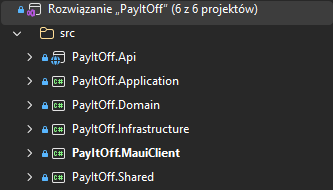
\includegraphics[width=0.45\textwidth]{img/widok_projektu.png}
    \captionof{figure}{Drzewo projektu w środowisku Visual Studio.}
\end{center}

\section{Specyfikacja REST API}
Aplikacja .NET MAUI działa jako bezstanowy klient. Cała logika biznesowa wykonywana jest bezpiecznie po stronie serwera API. Komunikacja odbywa się z wykorzystaniem protokołu HTTP, a wymiana informacji bazuje na obiektach w formacie JSON (Data Transfer Objects). Dostęp do większości zasobów wymaga nagłówka \texttt{Authorization: Bearer <token>}.

Dzięki zastosowaniu standardu OpenAPI i potężnego narzędzia \textbf{Swagger UI}, cała interaktywna dokumentacja punktów końcowych (wraz z wylistowanymi wszystkimi modelami DTO) jest dostępna graficznie z poziomu przeglądarki pod adresem \texttt{/swagger}. Pozwala to na wygodne testowanie żądań bez konieczności używania zewnętrznych narzędzi typu Postman.

\begin{center}
    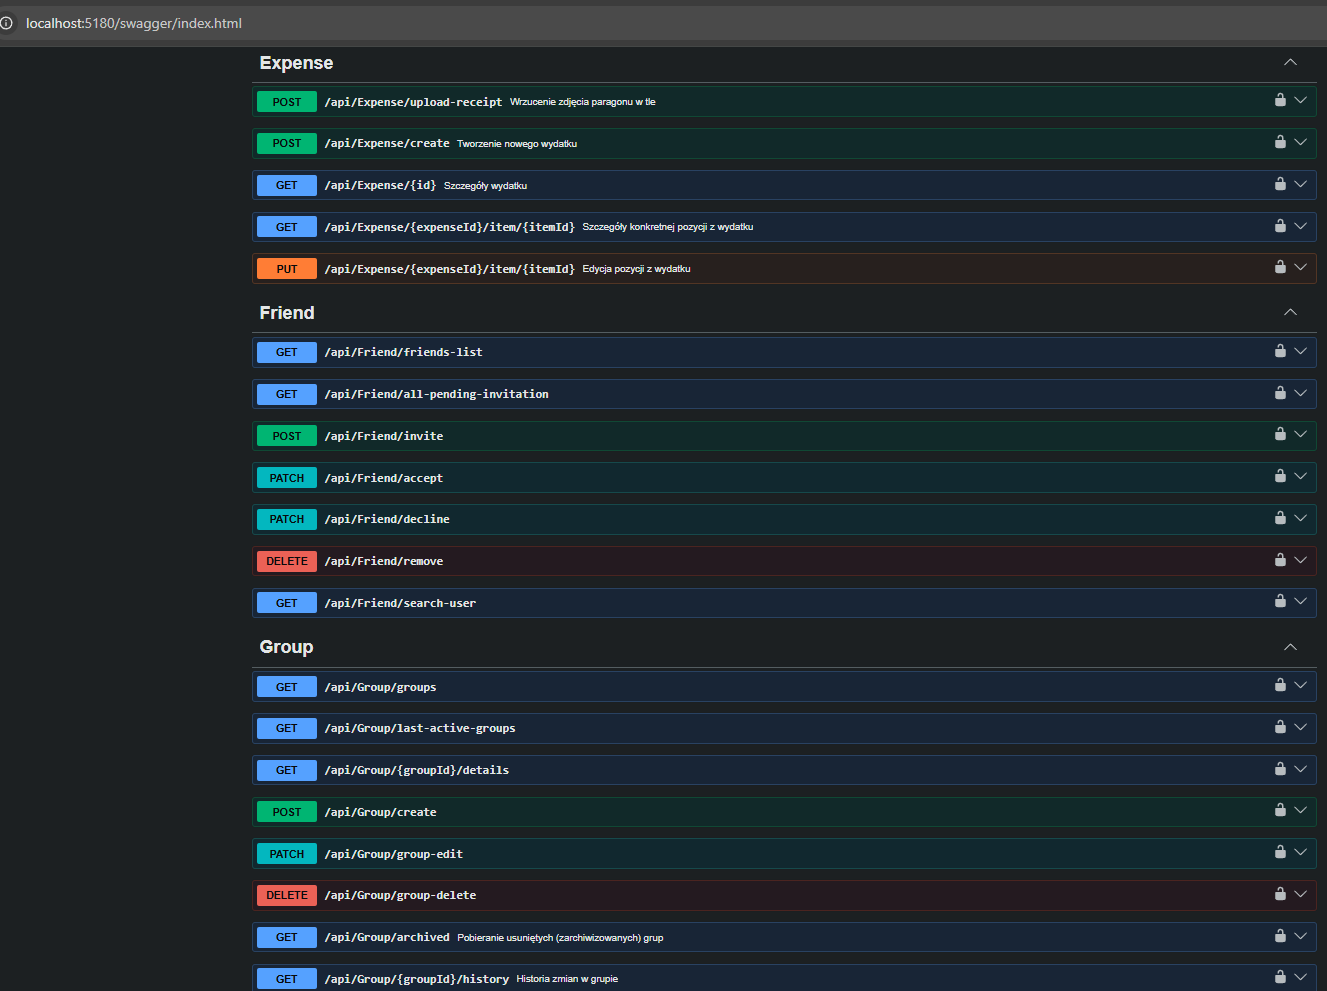
\includegraphics[width=0.95\textwidth]{img/swagger1.png}
    \captionof{figure}{Interfejs Swagger API – część 1. Zestawienie podstawowych operacji CRUD dla domen: \textbf{Expense} (zarządzanie paragonami), \textbf{Friend} (sieć znajomych) oraz \textbf{Group} (środowiska współdzielone).}
\end{center}

\begin{center}
    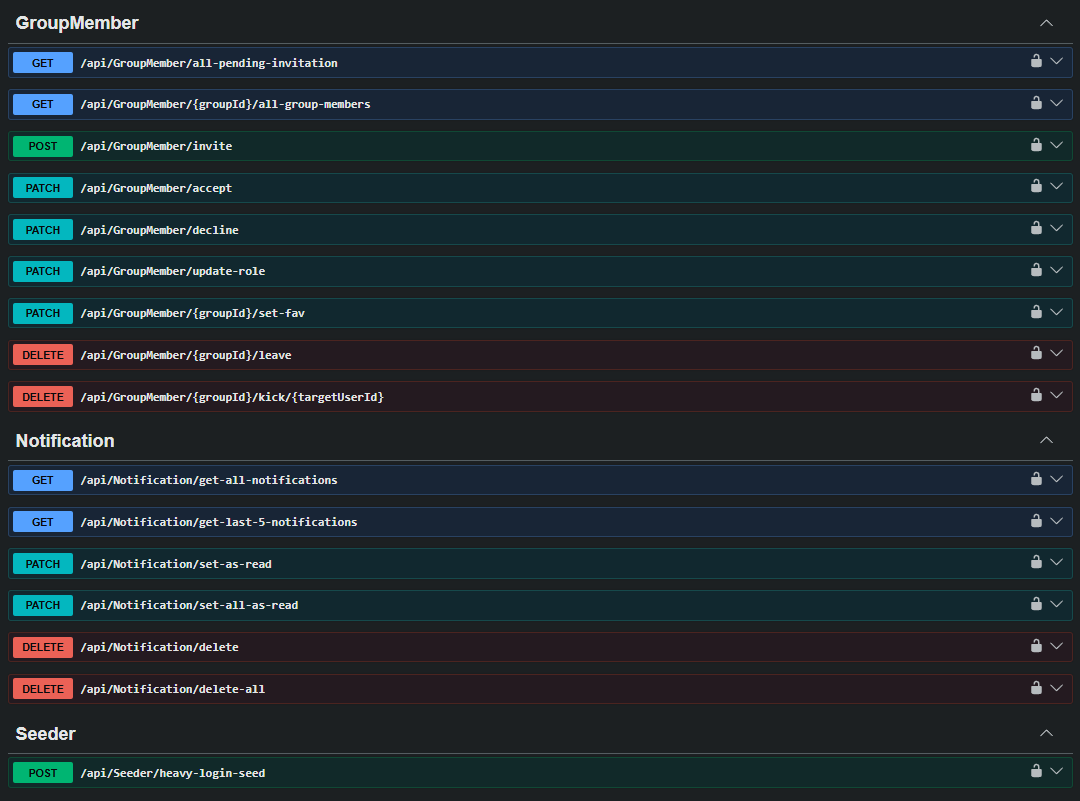
\includegraphics[width=0.95\textwidth]{img/swagger2.png}
    \captionof{figure}{Interfejs Swagger API – część 2. Punkty końcowe operujące na relacjach: \textbf{GroupMember} (role, uprawnienia), \textbf{Notification} (system powiadomień) oraz \textbf{Seeder} (wstrzykiwanie danych testowych).}
\end{center}

\begin{center}
    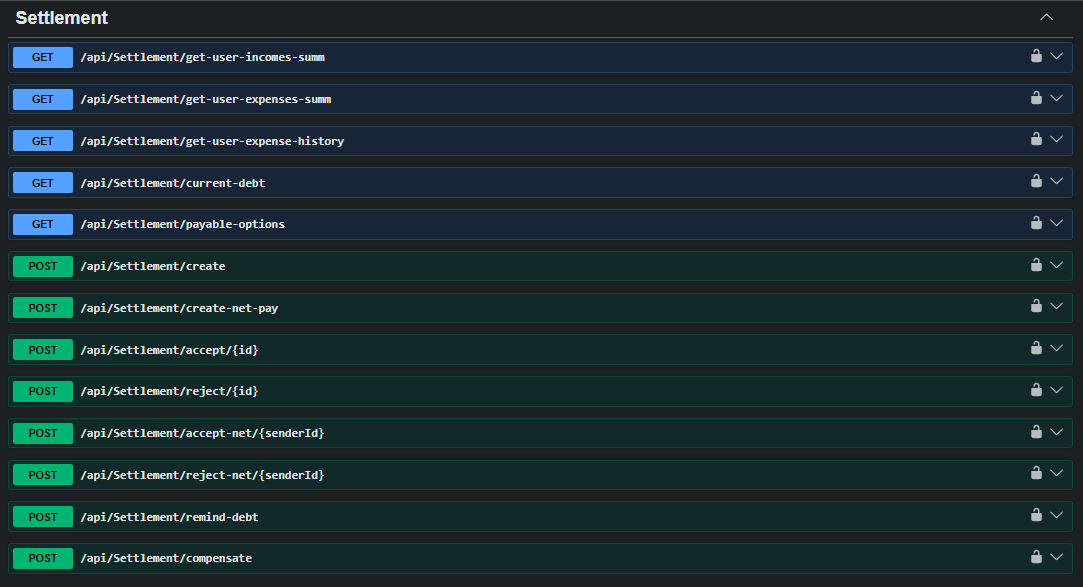
\includegraphics[width=0.95\textwidth]{img/swagger3.png}
    \captionof{figure}{Interfejs Swagger API – część 3. Główny silnik finansowy reprezentowany przez sekcję \textbf{Settlement}. Odpowiada za cały obieg pieniądza, deklaracje przelewów i kompensatę grafu zobowiązań.}
\end{center}

\begin{center}
    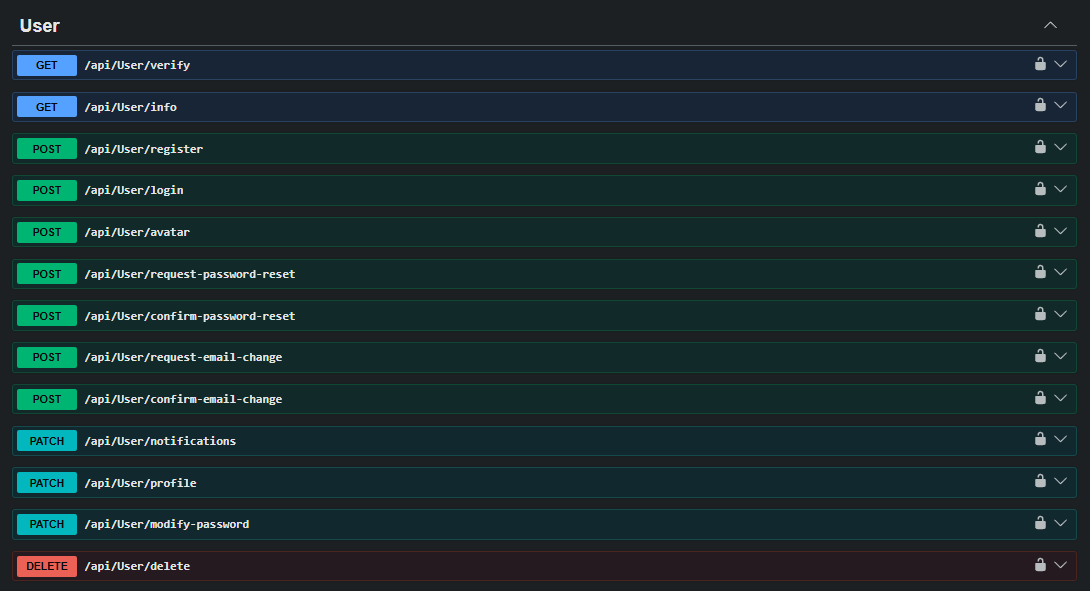
\includegraphics[width=0.95\textwidth]{img/swagger4.png}
    \captionof{figure}{Interfejs Swagger API – część 4. Moduł autoryzacji \textbf{User}. Punkty końcowe obsługujące rejestrację, uwierzytelnianie (JWT) oraz modyfikację wrażliwych danych konta.}
\end{center}

\section{Opis Bazy Danych}
\subsection{Schemat bazy (Diagram ERD)}
Baza danych składa się w sumie z 11 tabel połączonych odpowiednimi relacjami. Całość została zaprojektowana zgodnie z podejściem Code-First (baza generowana bezpośrednio z klas C\#).

\begin{center}
    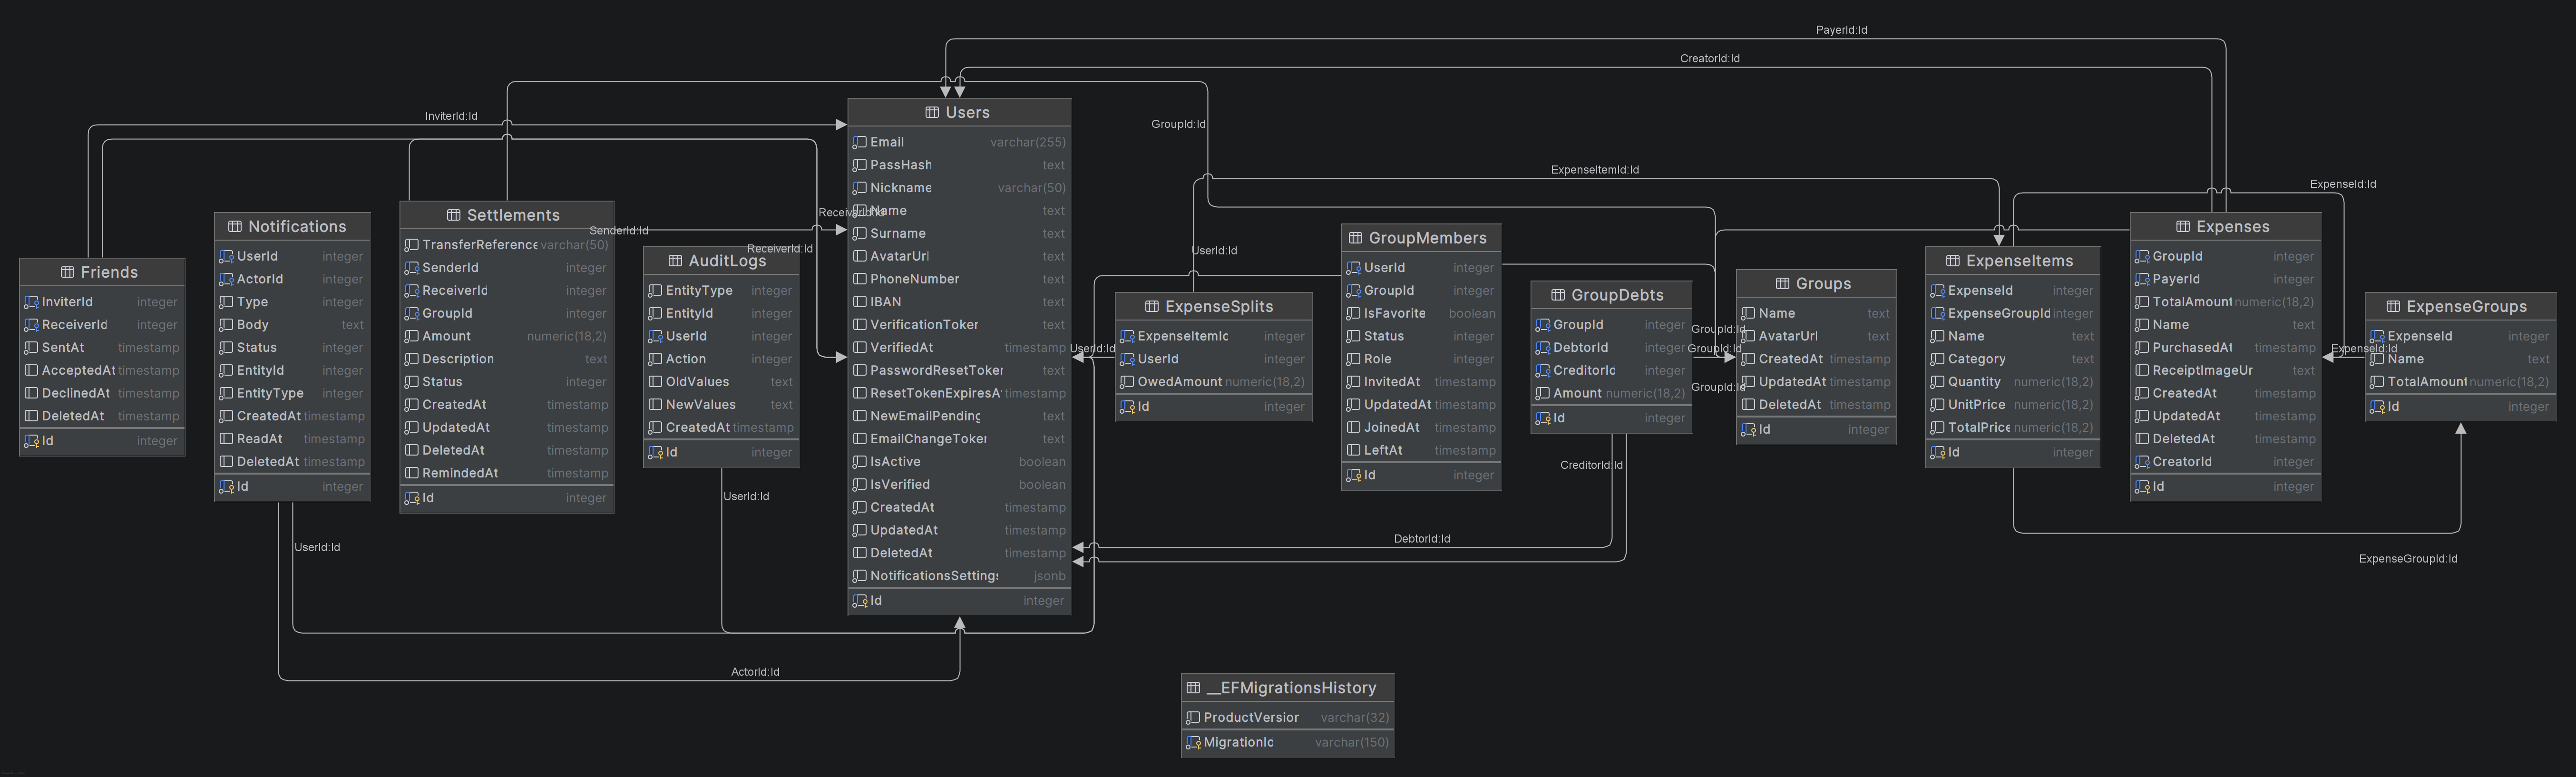
\includegraphics[width=0.95\textwidth]{img/diagram_erd.png}
    \captionof{figure}{Kompletny diagram związków encji (ERD) obrazujący architekturę relacyjnej bazy danych systemu PayItOff. Widoczne powiązania kluczy obcych i tabele łącznikowe.}
\end{center}

\subsection{Opis poszczególnych tabel}

\begin{center}
    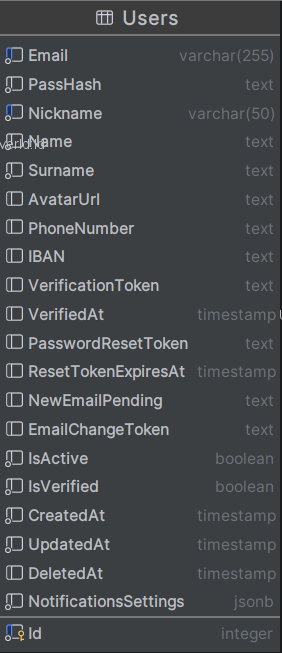
\includegraphics[width=0.45\textwidth]{img/tabele/Users.png}
    \hfill
    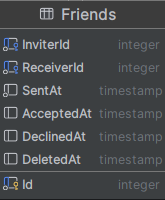
\includegraphics[width=0.45\textwidth]{img/tabele/Friends.png}
    \captionof{figure}{Struktura tabel \textbf{Users} oraz \textbf{Friends}. Po lewej główny agregat tożsamości z ustawieniami powiadomień. Po prawej tabela łącznikowa realizująca relację sieci kontaktów (Many-to-Many).}
\end{center}

\begin{center}
    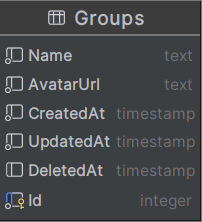
\includegraphics[width=0.45\textwidth]{img/tabele/Groups.png}
    \hfill
    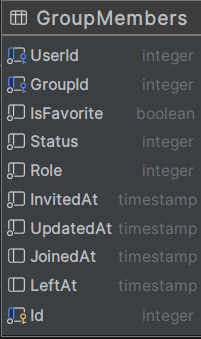
\includegraphics[width=0.45\textwidth]{img/tabele/GroupMembers.png}
    \captionof{figure}{Struktura środowisk współdzielonych. Tabela \textbf{Groups} realizuje miękkie usuwanie (DeletedAt), a \textbf{GroupMembers} odpowiada za kontrolę dostępu i przypisywanie ról (RBAC).}
\end{center}

\begin{center}
    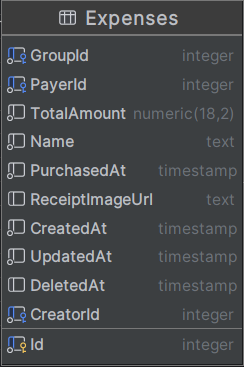
\includegraphics[width=0.45\textwidth]{img/tabele/Expenses.png}
    \hfill
    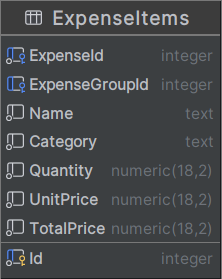
\includegraphics[width=0.45\textwidth]{img/tabele/ExpenseItems.png}
    \captionof{figure}{Modelowanie rachunków. Tabela \textbf{Expenses} przechowuje globalne metadane wydatku, natomiast \textbf{ExpenseItems} pozwala na szczegółowe rozbicie paragonu na pojedyncze produkty.}
\end{center}

\begin{center}
    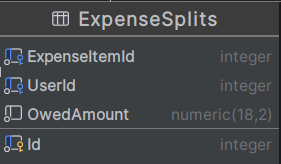
\includegraphics[width=0.45\textwidth]{img/tabele/ExpenseSplits.png}
    \hfill
    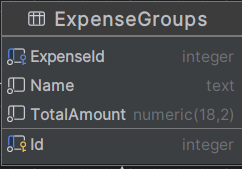
\includegraphics[width=0.45\textwidth]{img/tabele/ExpenseGroups.png}
    \captionof{figure}{Tabela \textbf{ExpenseSplits} to kluczowy punkt obliczeniowy dla przydziału należności ułamkowych (rozwiązanie Penny-Drop). \textbf{ExpenseGroups} wspomaga analitykę i kategoryzację.}
\end{center}

\begin{center}
    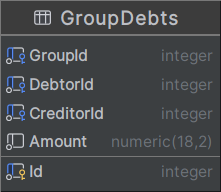
\includegraphics[width=0.45\textwidth]{img/tabele/GroupDebts.png}
    \hfill
    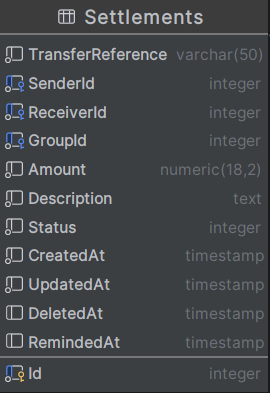
\includegraphics[width=0.45\textwidth]{img/tabele/Settlements.png}
    \captionof{figure}{Mechanizmy windykacyjne. \textbf{GroupDebts} to zdenormalizowany bufor odciążający bazę danych przy wyliczaniu grafu. \textbf{Settlements} zabezpiecza transakcje i transfery wyrównujące.}
\end{center}

\begin{center}
    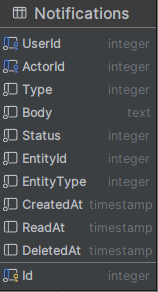
\includegraphics[width=0.45\textwidth]{img/tabele/Notifications.png}
    \hfill
    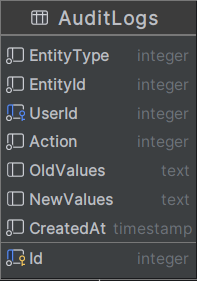
\includegraphics[width=0.45\textwidth]{img/tabele/AuditLogs.png}
    \captionof{figure}{Zdarzenia i bezpieczeństwo. \textbf{Notifications} utrzymuje stan odczytu asynchronicznych powiadomień. \textbf{AuditLogs} realizuje wzorzec Audit Trail logując wszystkie historyczne modyfikacje.}
\end{center}

\section{Wygląd i przepływ w aplikacji (.NET MAUI)}
Poniższa sekcja prezentuje interfejs graficzny aplikacji zreorganizowany w pełni chronologicznie. Pokazuje ona naturalną ścieżkę użytkownika (User Journey) – od pierwszego uruchomienia aplikacji i budowania sieci kontaktów, przez tworzenie grup i wprowadzanie kosztów, aż po ostateczne rozliczenia długów oraz zarządzanie retencją danych (usuwanie profilu).

\subsection{Krok 1: Inicjacja (Rejestracja i Logowanie)}
Proces rozpoczyna się od utworzenia nowego profilu w systemie, weryfikacji haseł, po czym następuje autoryzacja z użyciem zwalidowanych poświadczeń.

\begin{center}
    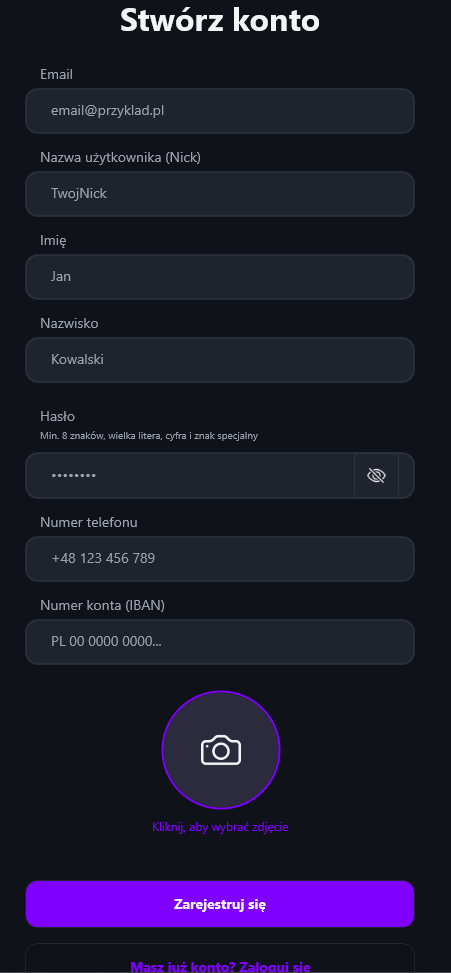
\includegraphics[width=0.45\textwidth]{img/register/register1.png}
    \hfill
    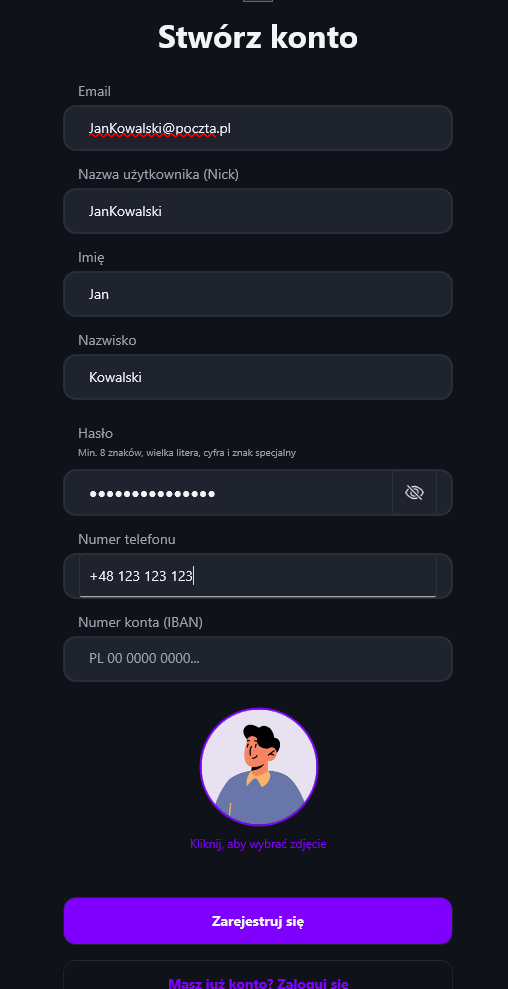
\includegraphics[width=0.45\textwidth]{img/register/register2.png}
    \captionof{figure}{Kolejne etapy formularza rejestracji konta użytkownika. Aplikacja zbiera i poddaje ścisłej walidacji podstawowe dane uwierzytelniające.}
\end{center}

\begin{center}
    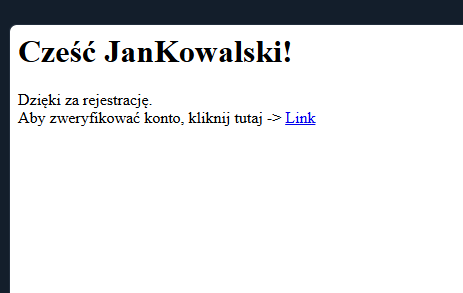
\includegraphics[width=0.45\textwidth]{img/register/register_mailtrapio.png}
    \hfill
    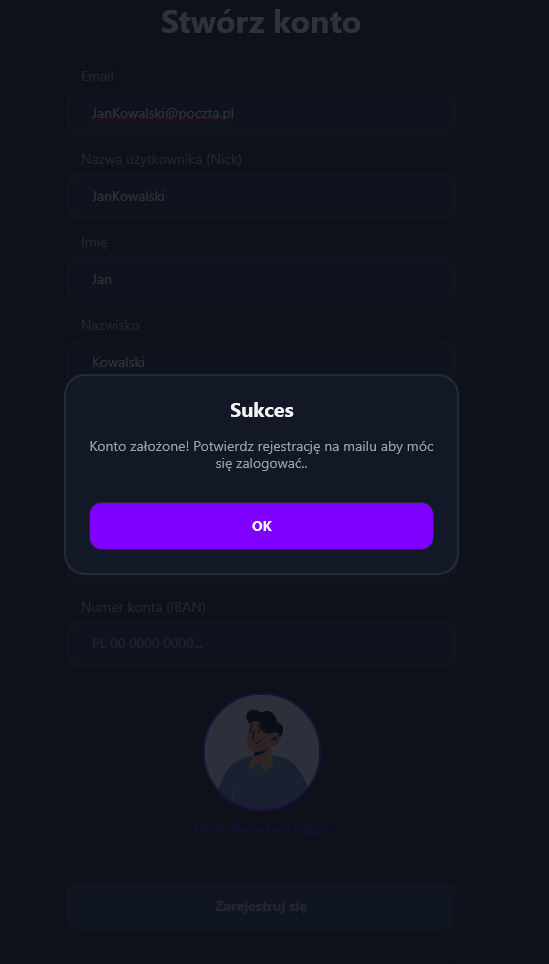
\includegraphics[width=0.45\textwidth]{img/register/register_success.png}
    \captionof{figure}{Proces weryfikacji e-mail. Widoczna symulacja skrzynki pocztowej (Mailtrap) z tokenem aktywacyjnym oraz ekran kończący rejestrację.}
\end{center}

\begin{center}
    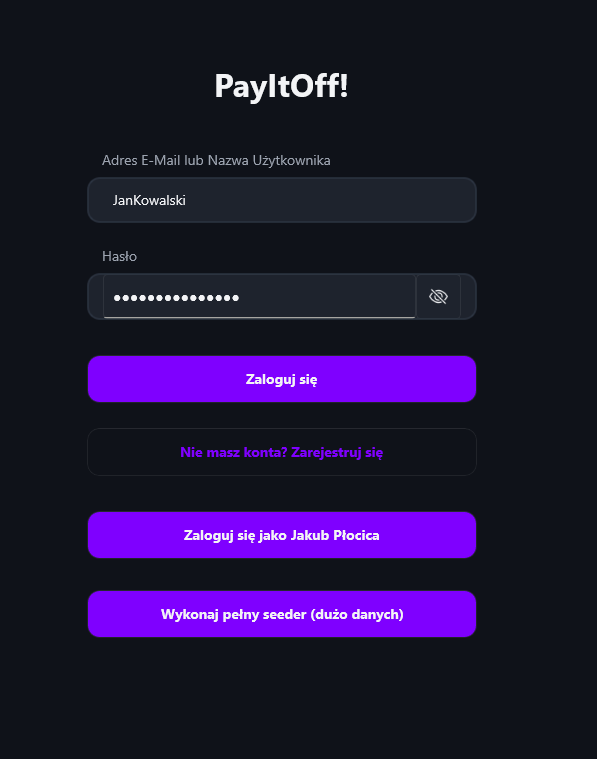
\includegraphics[width=0.45\textwidth]{img/login/login1.png}
    \hfill
    
\includegraphics[width=0.45\textwidth]{img/login/login_widoczne_haslo.png}
    \vspace{0.5cm} \\
    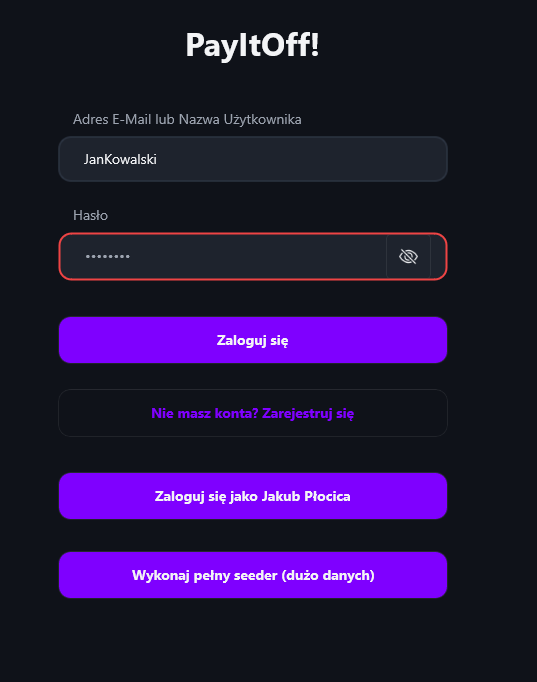
\includegraphics[width=0.45\textwidth]{img/login/login_error.png}
    \captionof{figure}{Moduł logowania. Widok z ukrytym hasłem, funkcja podglądu hasła w locie oraz mechanizm walidacji nieprawidłowych poświadczeń autoryzacyjnych.}
\end{center}


\subsection{Krok 2: Konfiguracja, Nawigacja i Zarządzanie Kontem}
Po pomyślnej autoryzacji system przekierowuje nas do głównego pulpitu. Otwiera się również dostęp do menu nawigacyjnego i edycji profilu (zmiana awatara, haseł, e-maila oraz usunięcie konta).

\begin{center}
    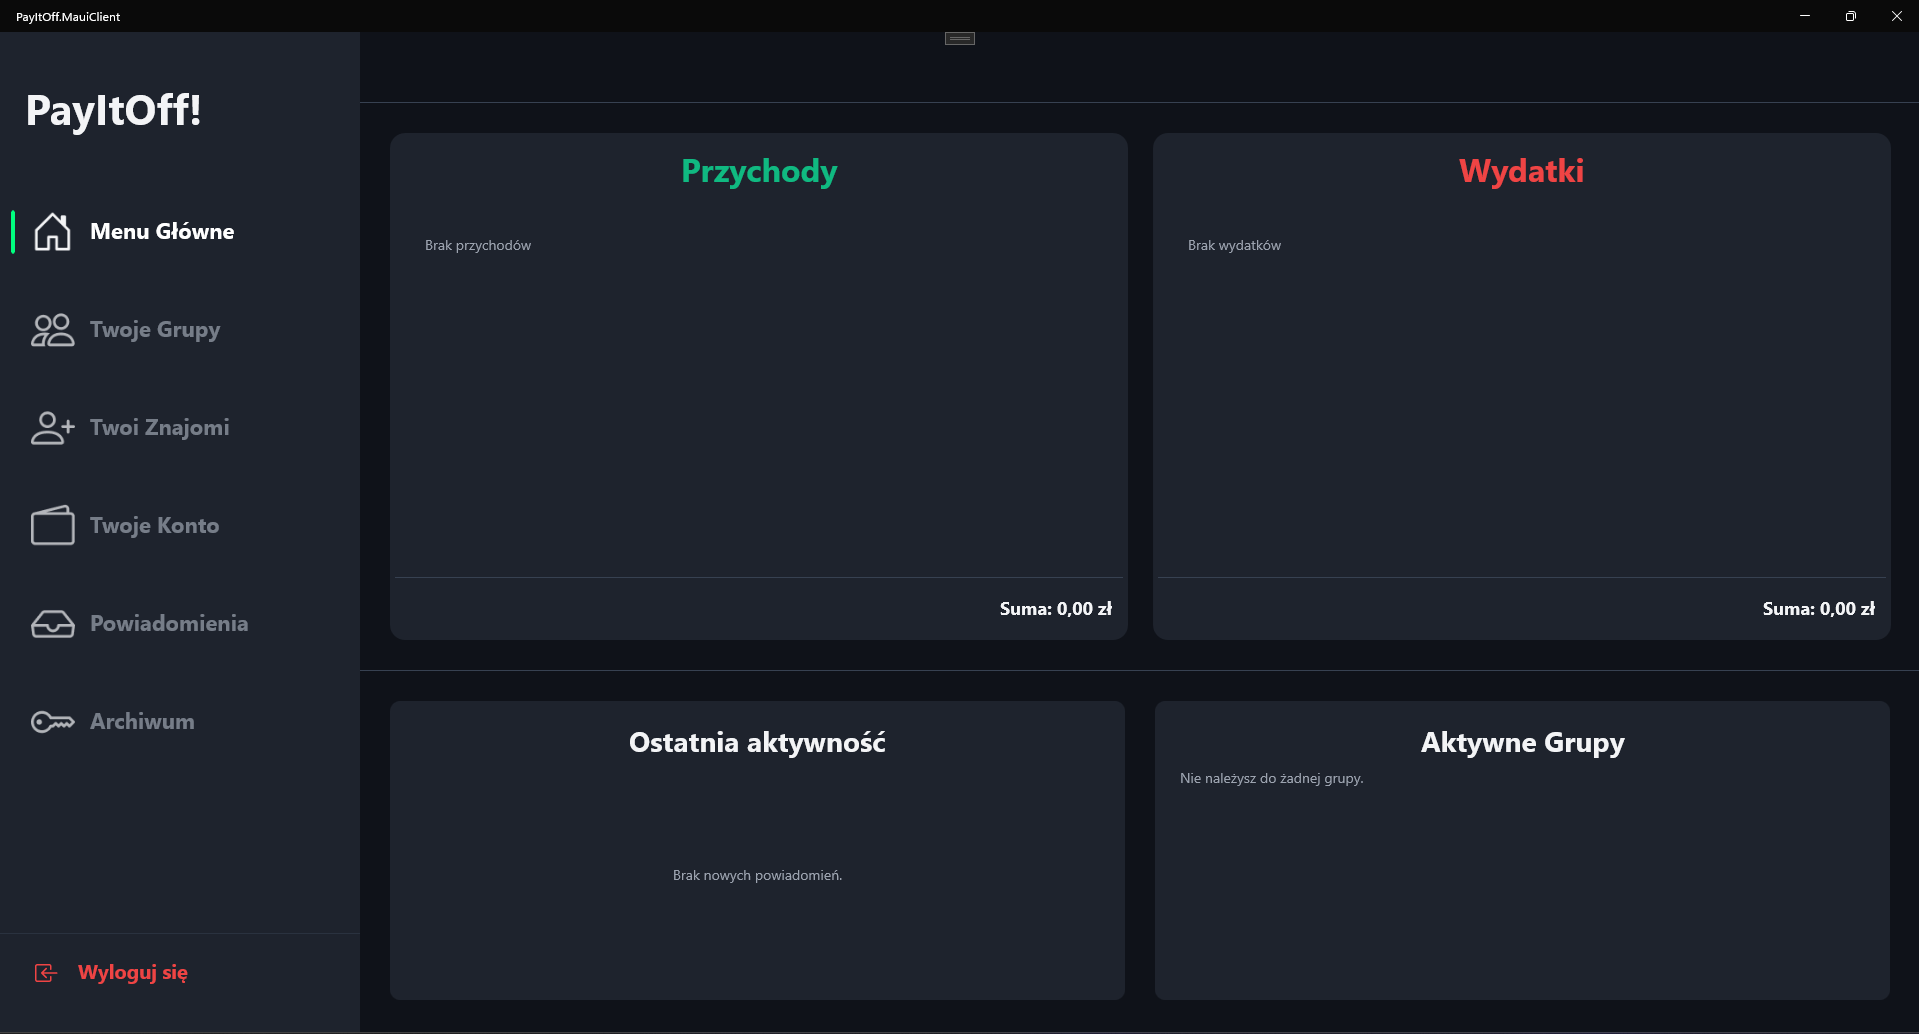
\includegraphics[width=0.95\textwidth]{img/main/main_pusty.png}
    \vspace{0.5cm} \\
    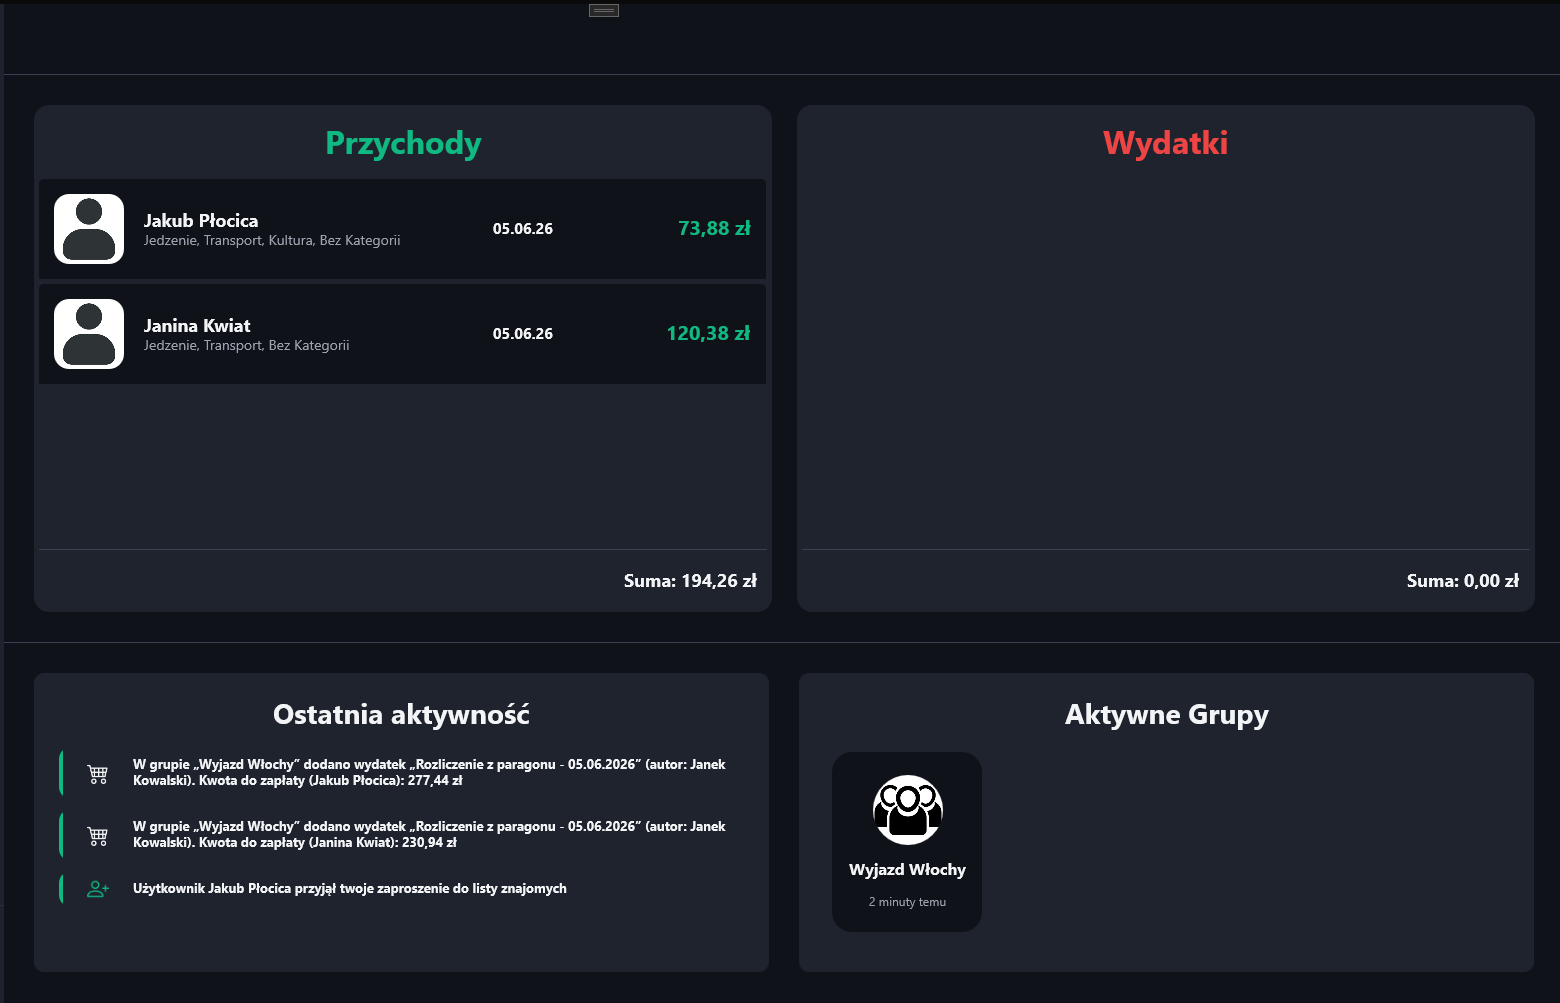
\includegraphics[width=0.95\textwidth]{img/main/main_po_dodaniu_wydatku.png}
    \vspace{0.5cm} \\
    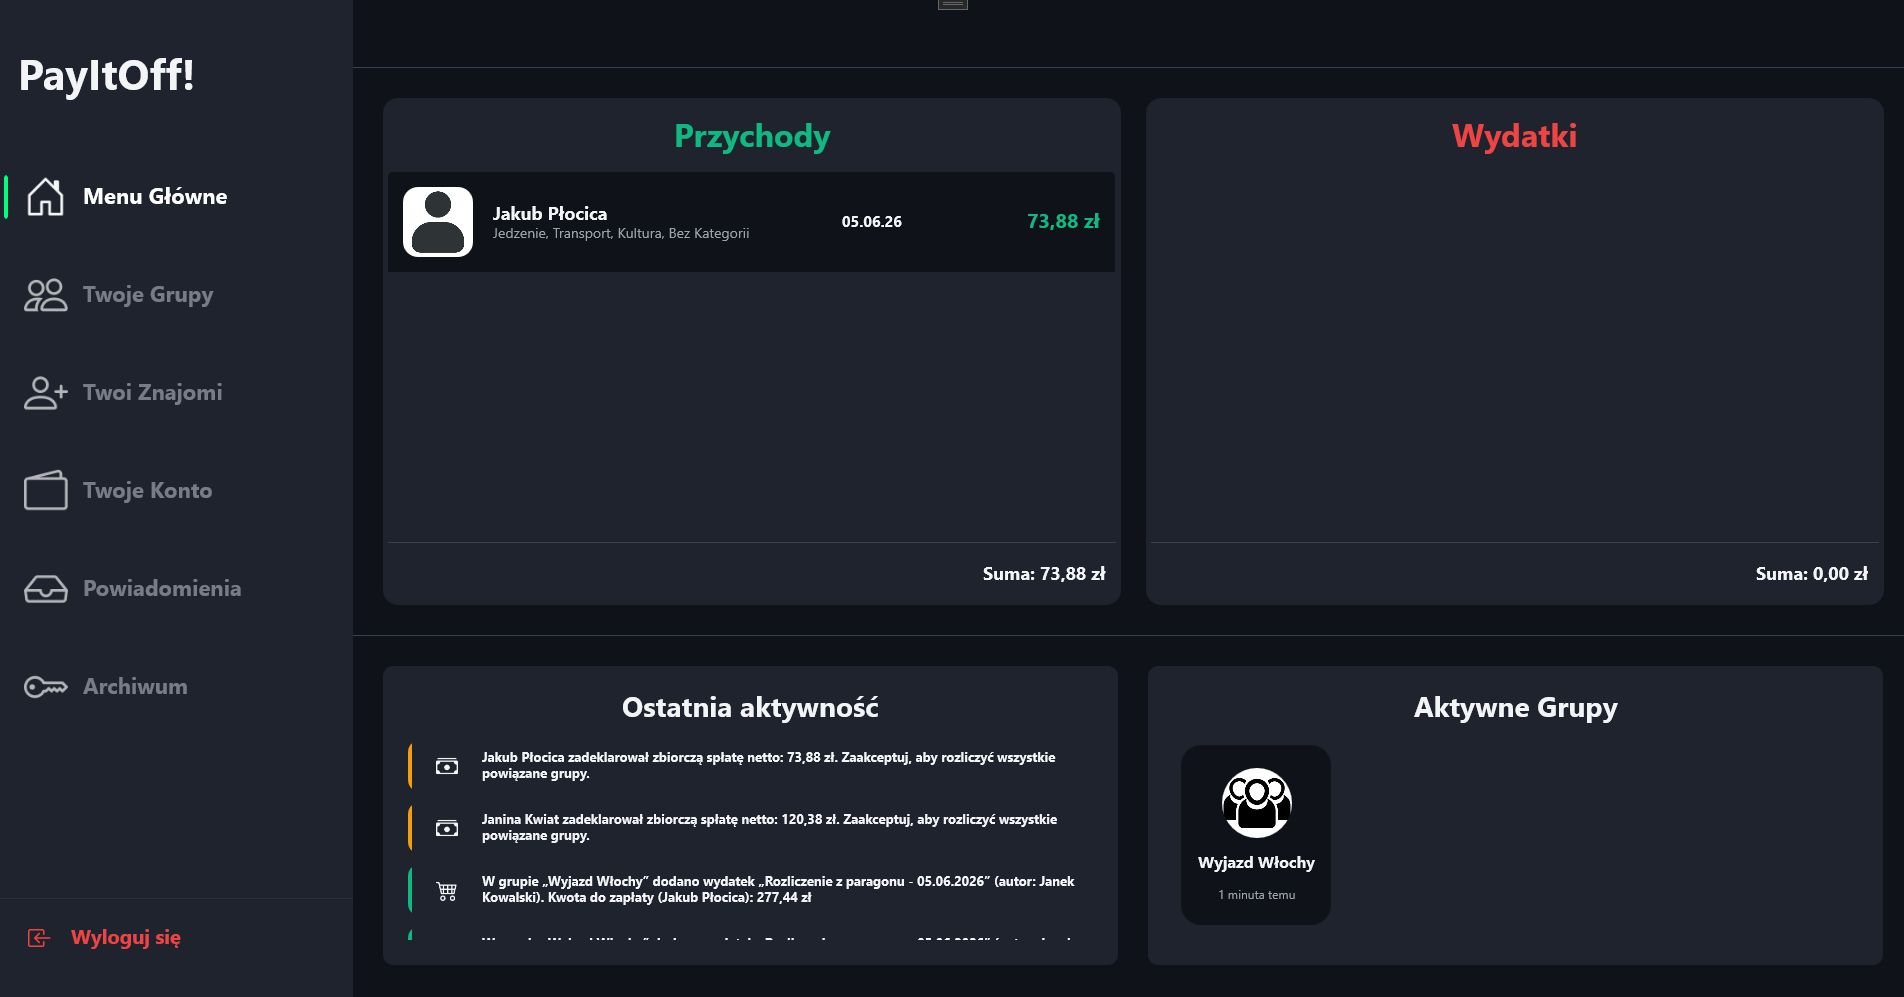
\includegraphics[width=0.95\textwidth]{img/main/main_po_akceptacji_i_odrzuceniu_splat.png}
    \captionof{figure}{Główny pulpit nawigacyjny (Dashboard). Od lewej: pusty stan początkowy, stan z aktywnością wydatkową oraz widok reagujący na spłaty i odrzucenia (zmiany na liście powiadomień).}
\end{center}

\begin{center}
    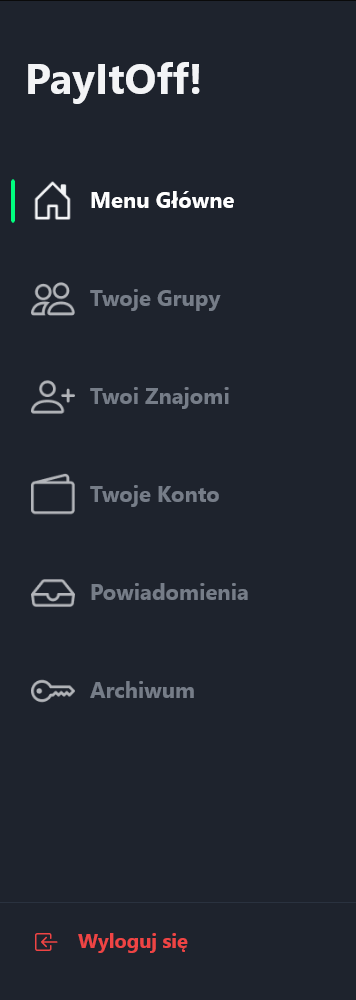
\includegraphics[width=0.45\textwidth]{img/sidebar.png}
    \vspace{0.5cm} \\
    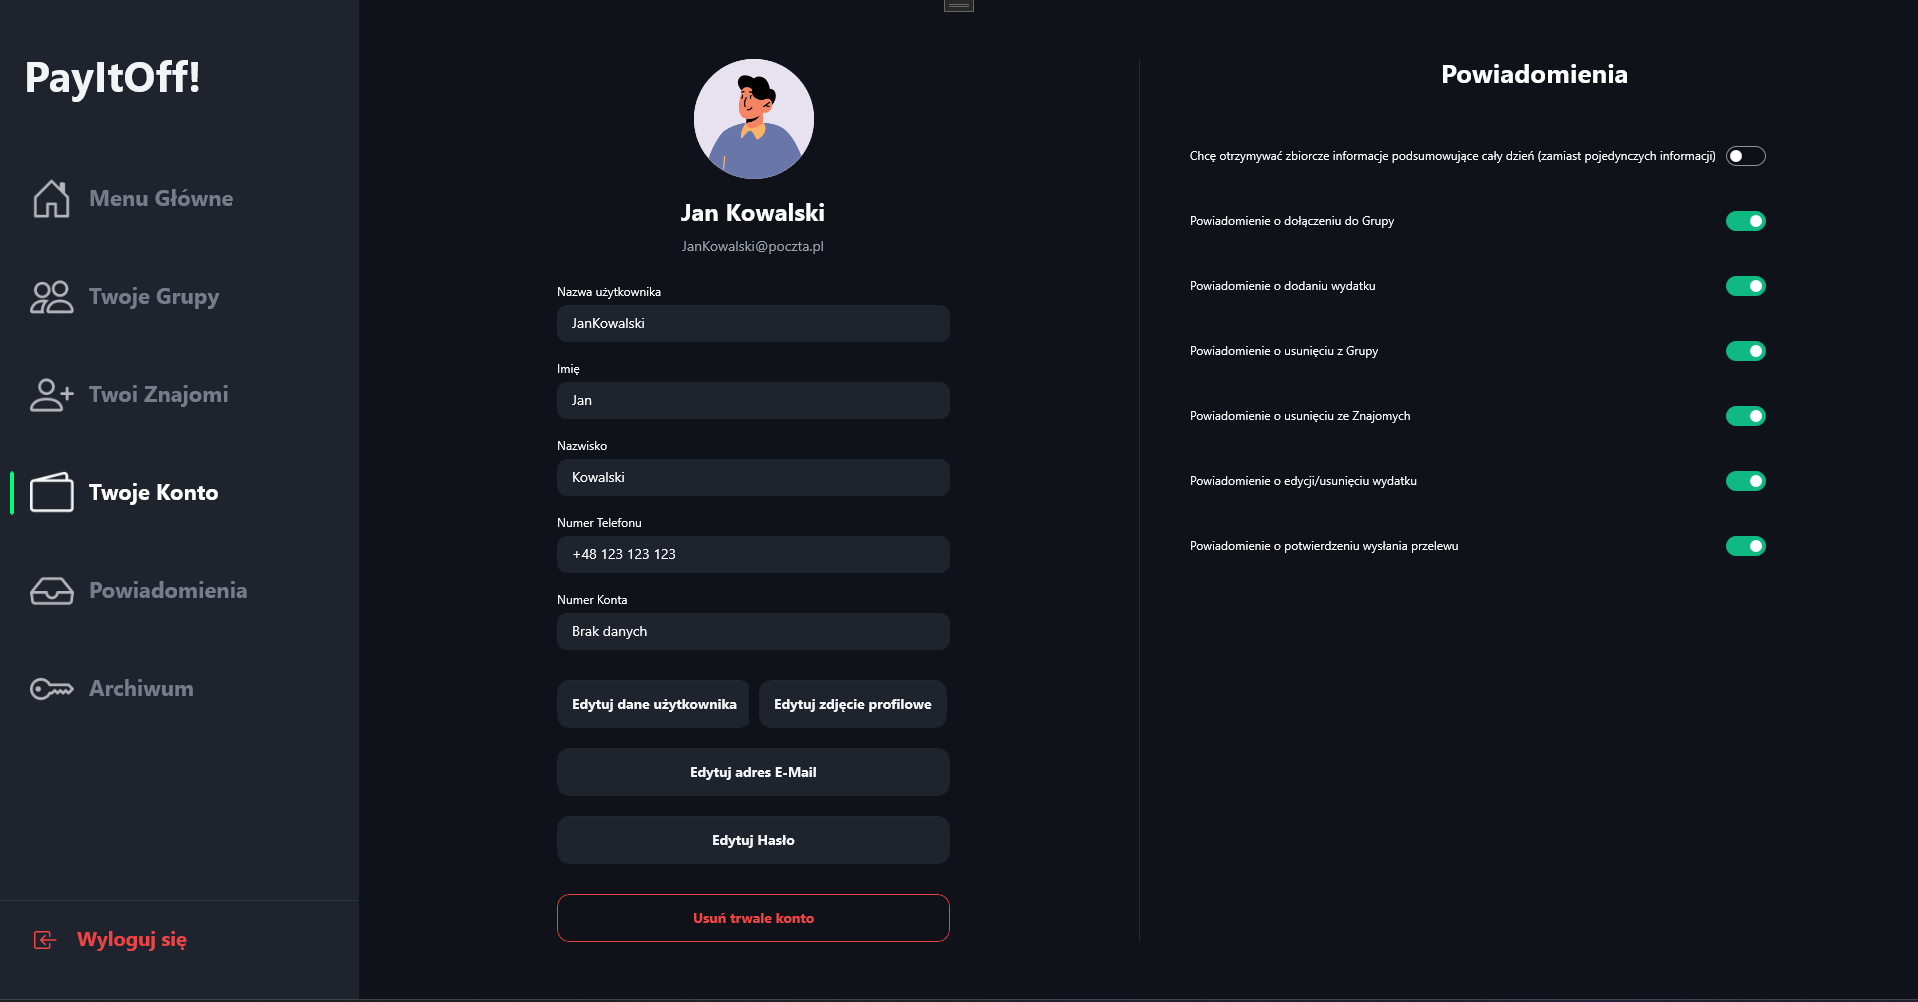
\includegraphics[width=0.95\textwidth]{img/account/account1.png}
    \vspace{0.5cm} \\
    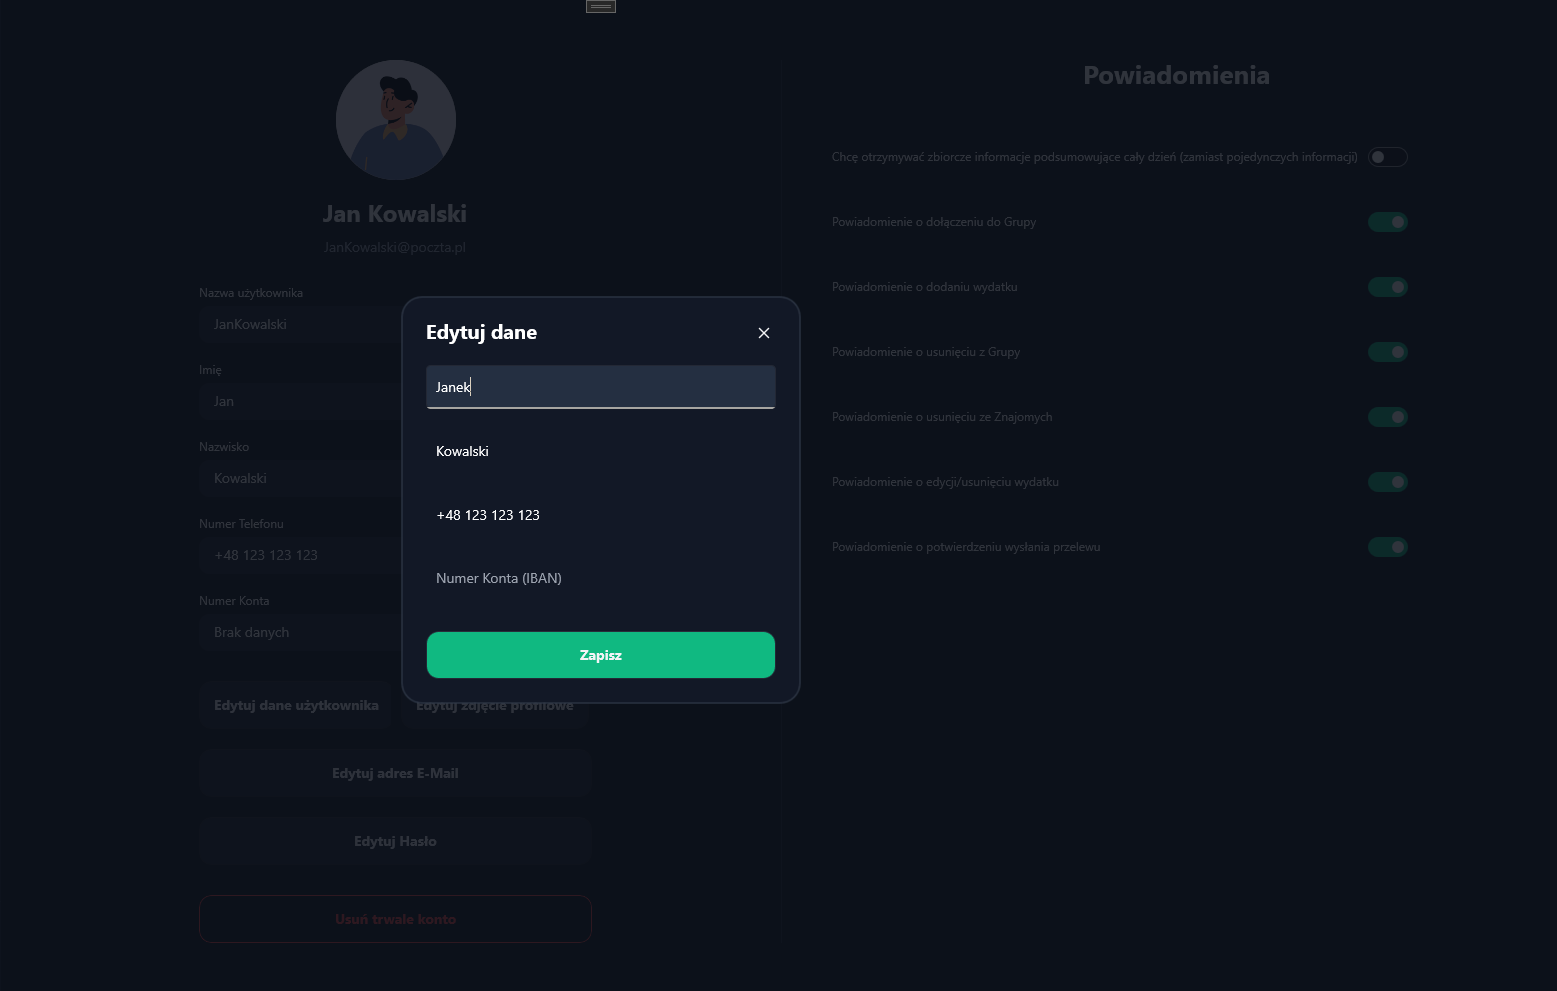
\includegraphics[width=0.95\textwidth]{img/account/account_zmiana_danych.png}
    \captionof{figure}{Rozwijane menu boczne (Sidebar) umożliwiające szybką nawigację oraz główny widok profilu z funkcją edycji podstawowych danych osobowych.}
\end{center}

\begin{center}
    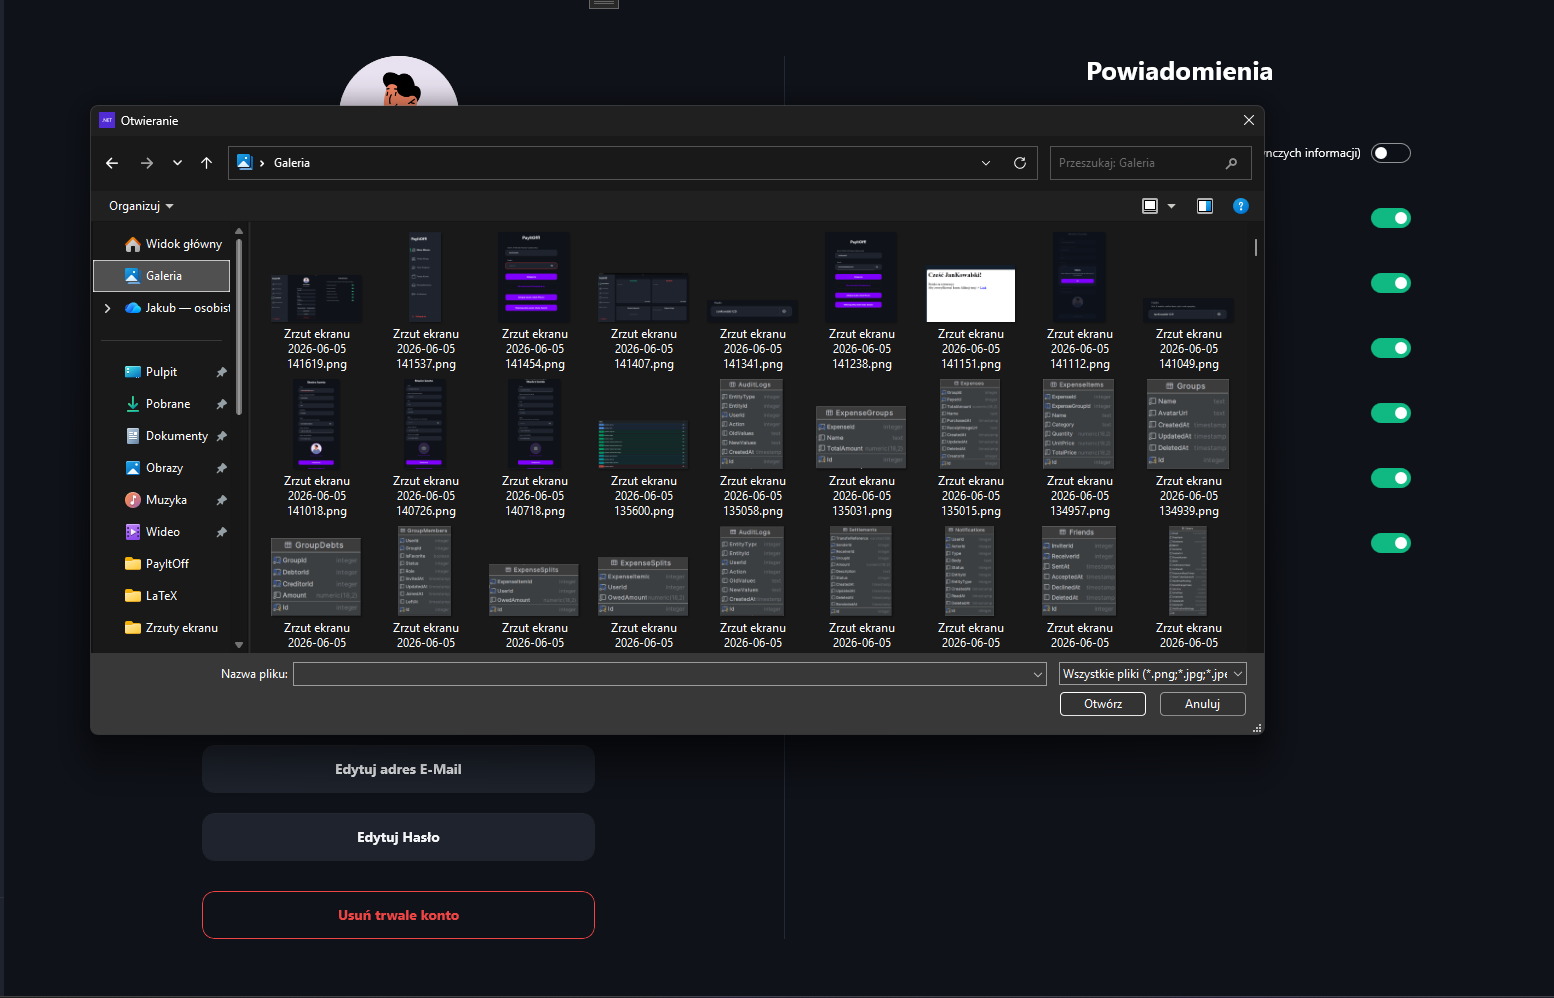
\includegraphics[width=0.95\textwidth]{img/account/account_zmiana_avatara.png}
    \vspace{0.5cm} \\
    
\includegraphics[width=0.45\textwidth]{img/account/account_zmienione_dane.png}
    \hfill
    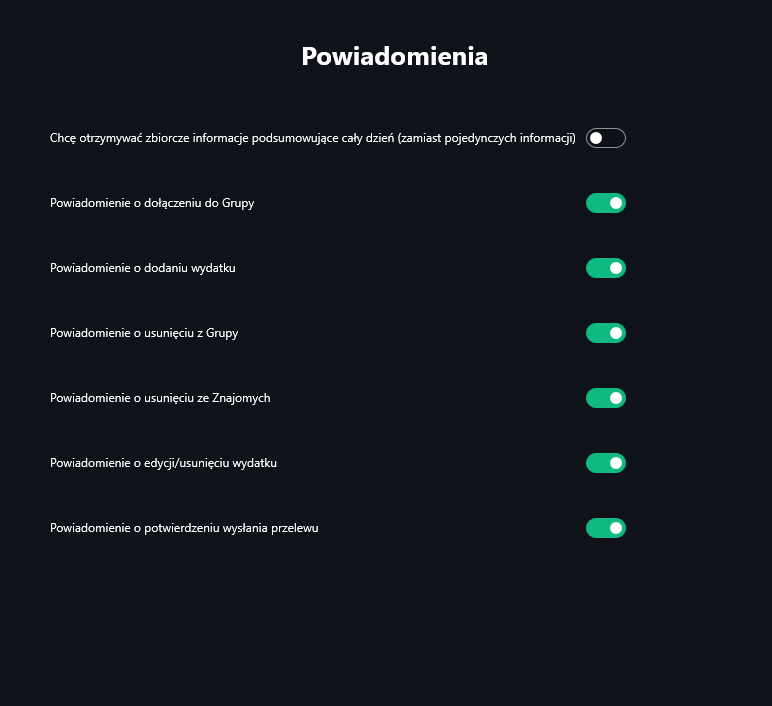
\includegraphics[width=0.45\textwidth]{img/account/account_edycja_ustawien_powiadomien.png}
    \captionof{figure}{Modyfikacja profilu. Przebieg zmiany zdjęcia profilowego (awatara), potwierdzenie wgrania danych oraz panel konfiguracji globalnych preferencji dla systemu notyfikacji.}
\end{center}

\begin{center}
    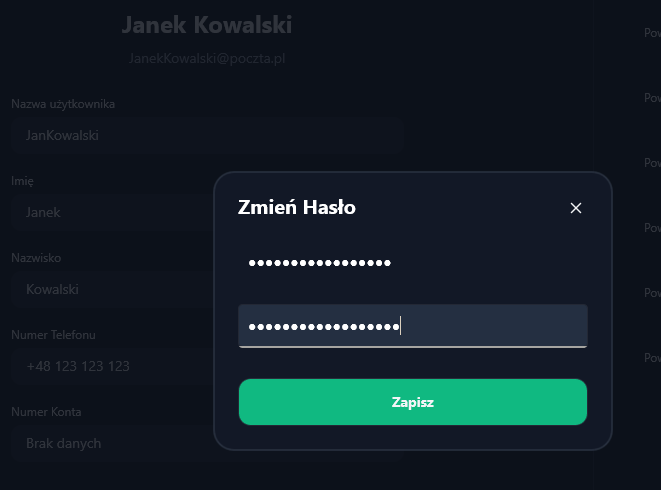
\includegraphics[width=0.45\textwidth]{img/account/account_zmiana_hasla.png}
    \hfill
    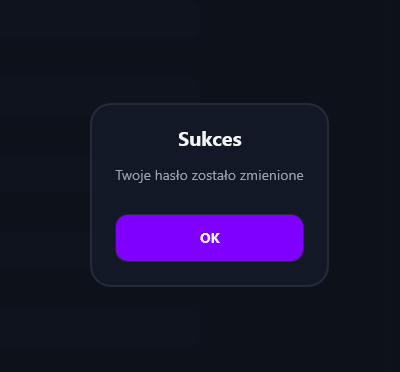
\includegraphics[width=0.45\textwidth]{img/account/account_zmiana_hasla_success.png}
    \vspace{0.5cm} \\
    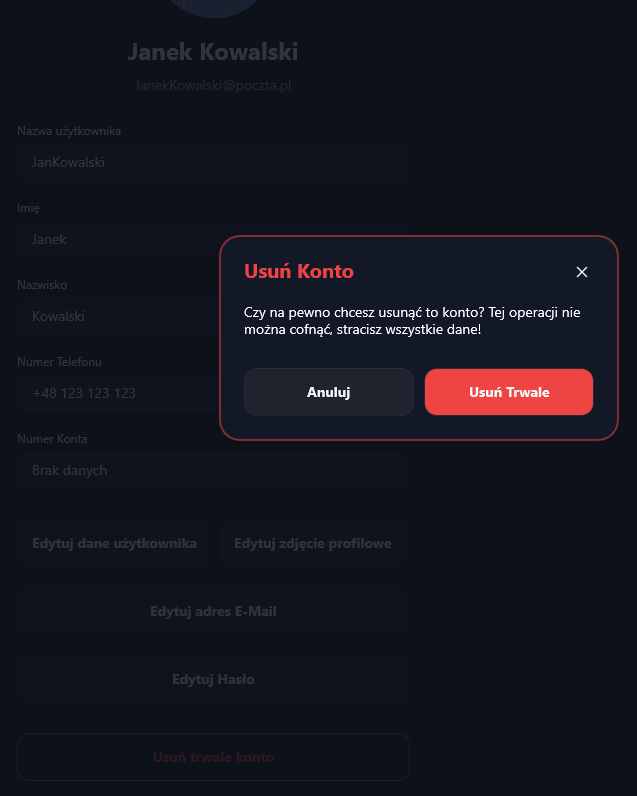
\includegraphics[width=0.45\textwidth]{img/account/account_usuniecie_konta.png}
    \captionof{figure}{Krytyczne operacje na profilu. Bezpieczna procedura zmiany hasła uwierzytelniającego oraz wywołanie formularza usunięcia konta (wiążącego się z weryfikacją zależności rozliczeniowych).}
\end{center}

\begin{center}
    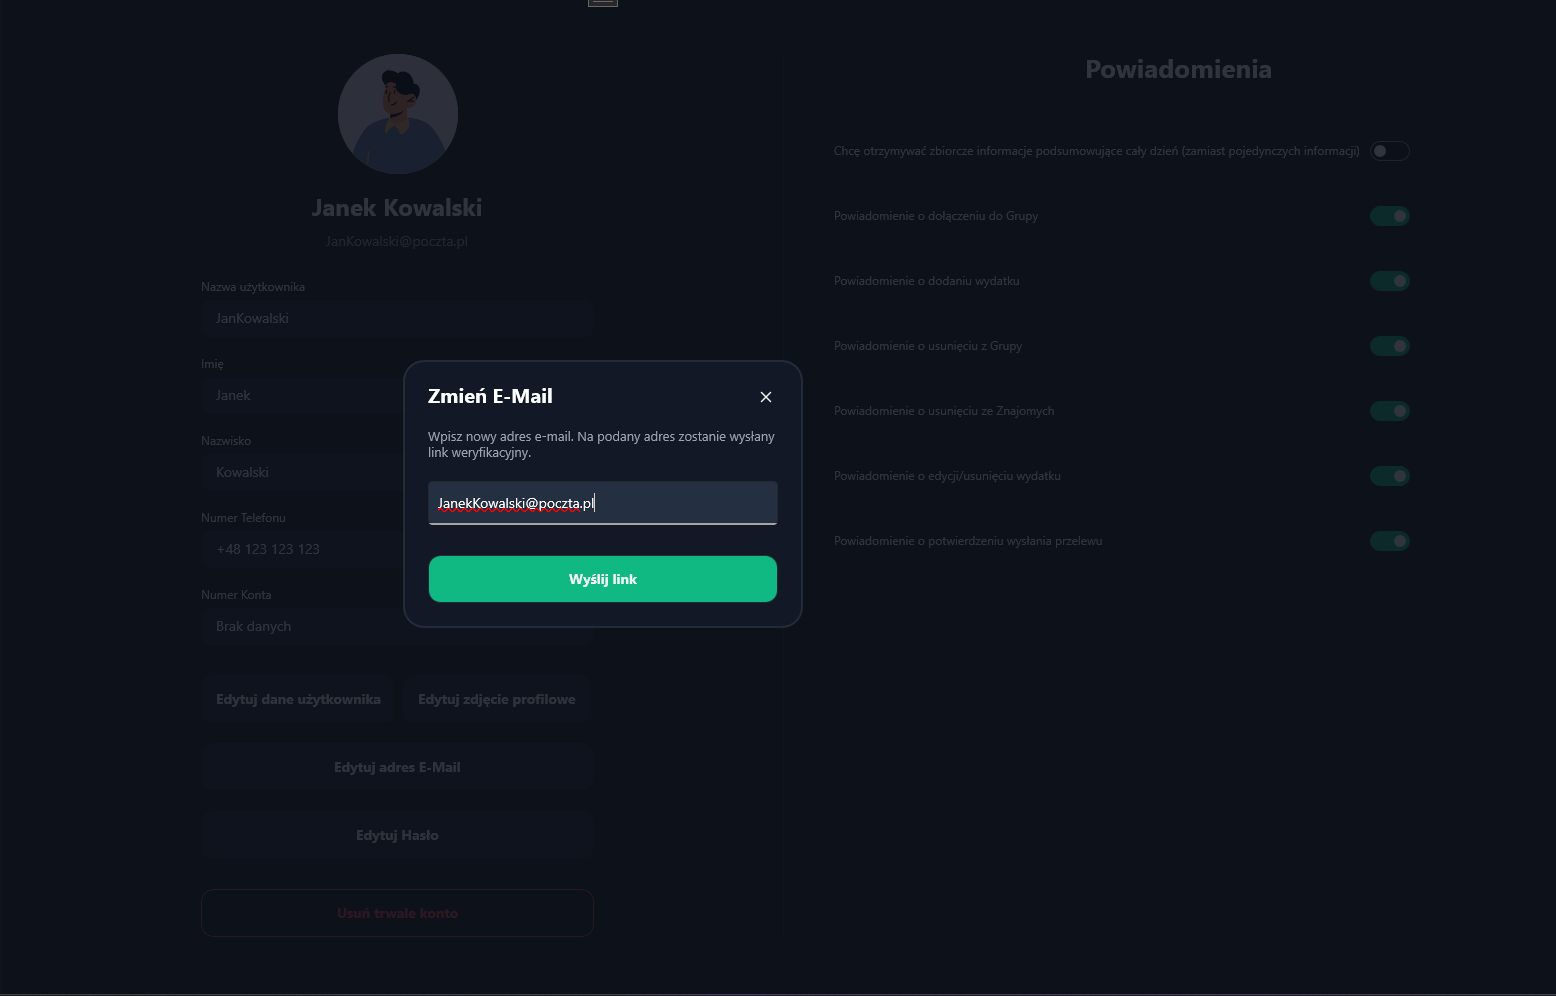
\includegraphics[width=0.95\textwidth]{img/account/account_zmiana_maila.png}
    \vspace{0.5cm} \\
    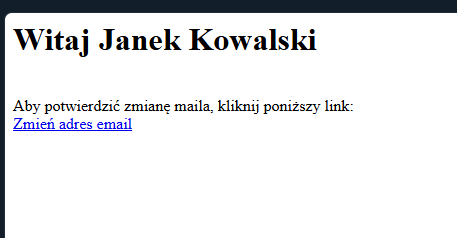
\includegraphics[width=0.45\textwidth]{img/account/account_zmiana_maila_mailtrapio.png}
    \captionof{figure}{Procedura modyfikacji adresu e-mail powiązana z wymogiem potwierdzenia dostępu. Skrzynka weryfikacyjna przechwytuje token zabezpieczający operację.}
\end{center}

\begin{center}
    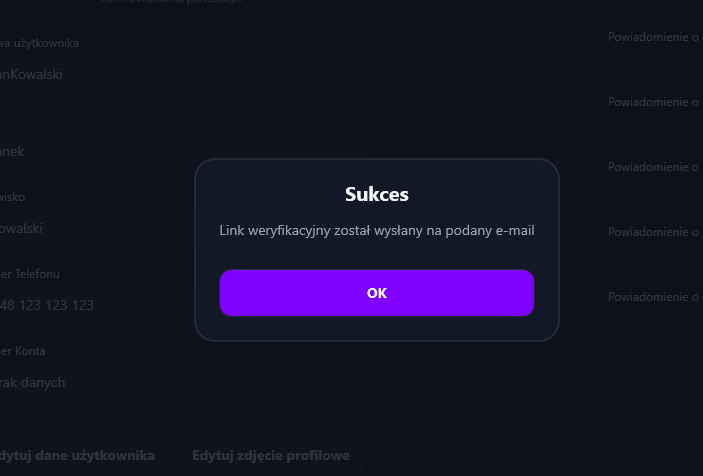
\includegraphics[width=0.45\textwidth]{img/account/account_zmiana_maila_success.png}
    \hfill
    
\includegraphics[width=0.45\textwidth]{img/account/zmiana_maila_faktyczna.png}
    \captionof{figure}{Zakończenie i zwalidowanie zmiany adresu e-mail, co natychmiast odświeża kontekst tożsamości we wbudowanych tokenach JWT.}
\end{center}


\subsection{Krok 3: Budowanie Sieci Kontaktów (Friends)}
Aplikacja zyskuje wartość dopiero w interakcji z innymi. Przed założeniem grupy, nawiązujemy relacje wyszukując znajomych i wysyłając im wirtualne zaproszenia do sieci.

\begin{center}
    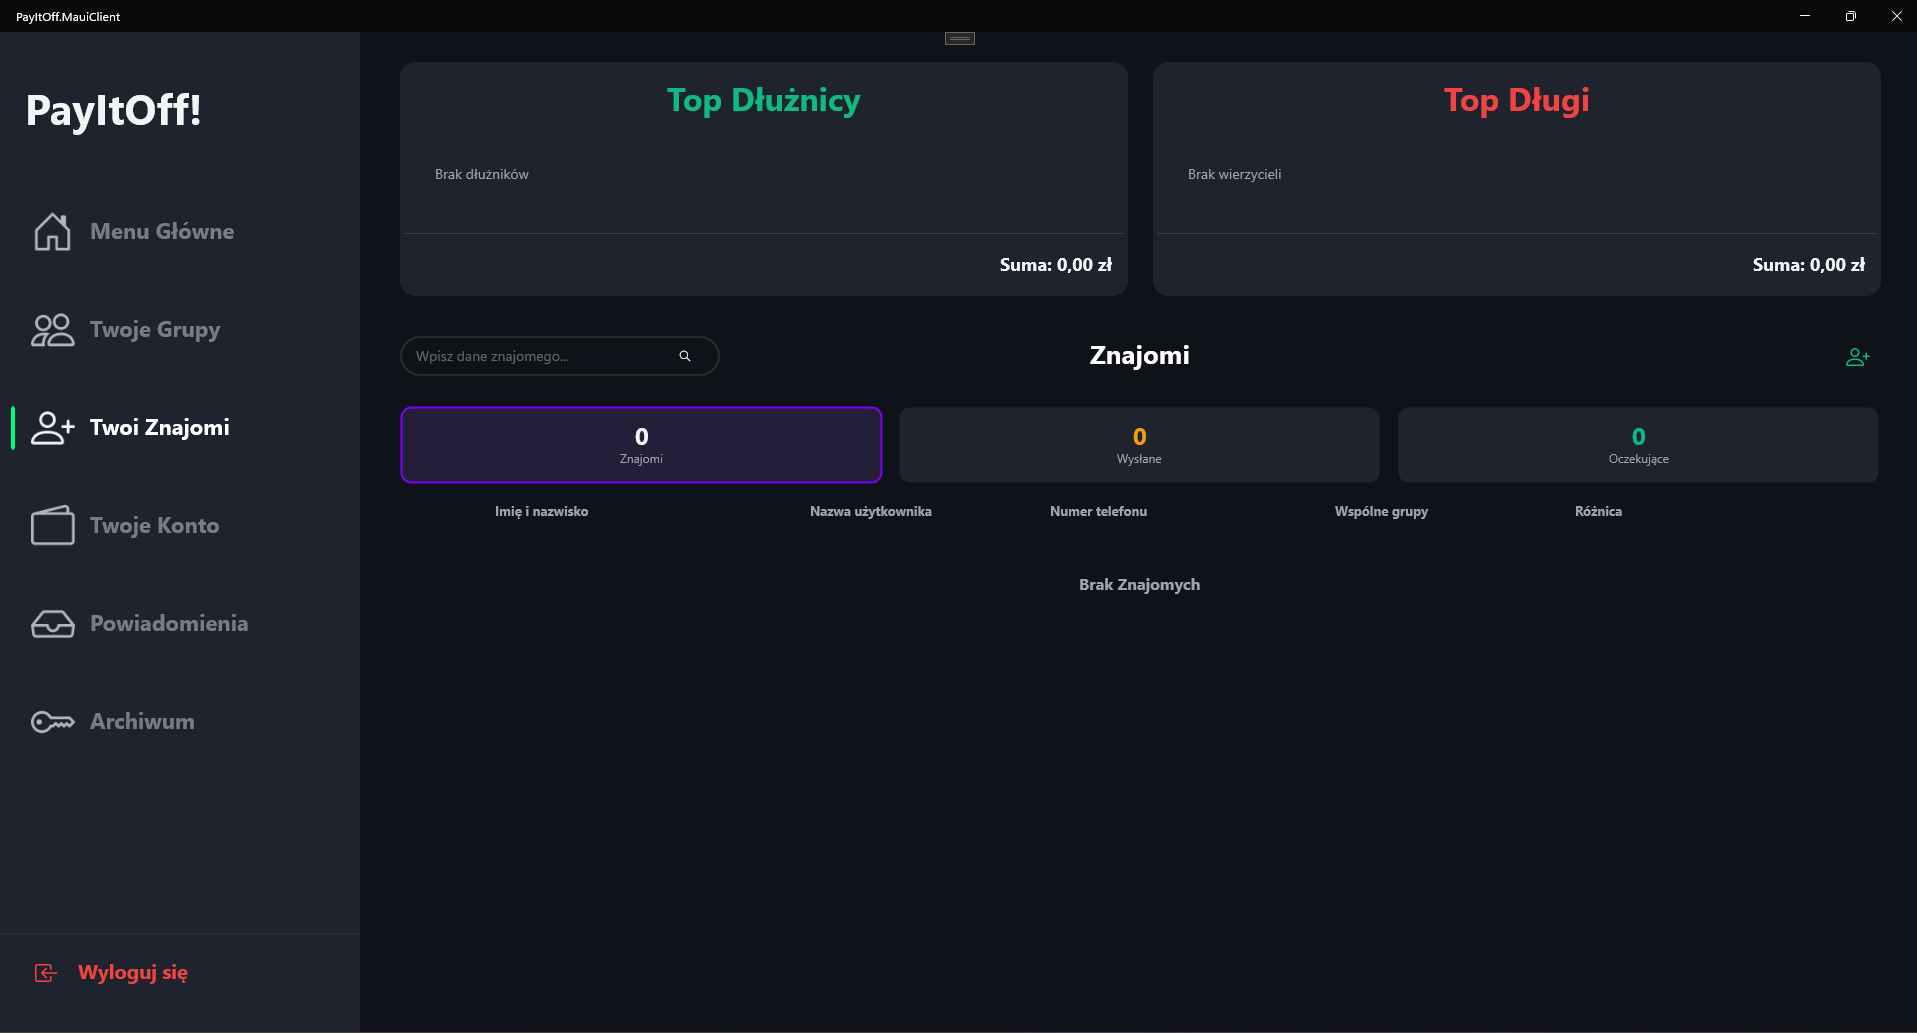
\includegraphics[width=0.95\textwidth]{img/friend/friend_puste.png}
    \vspace{0.5cm} \\
    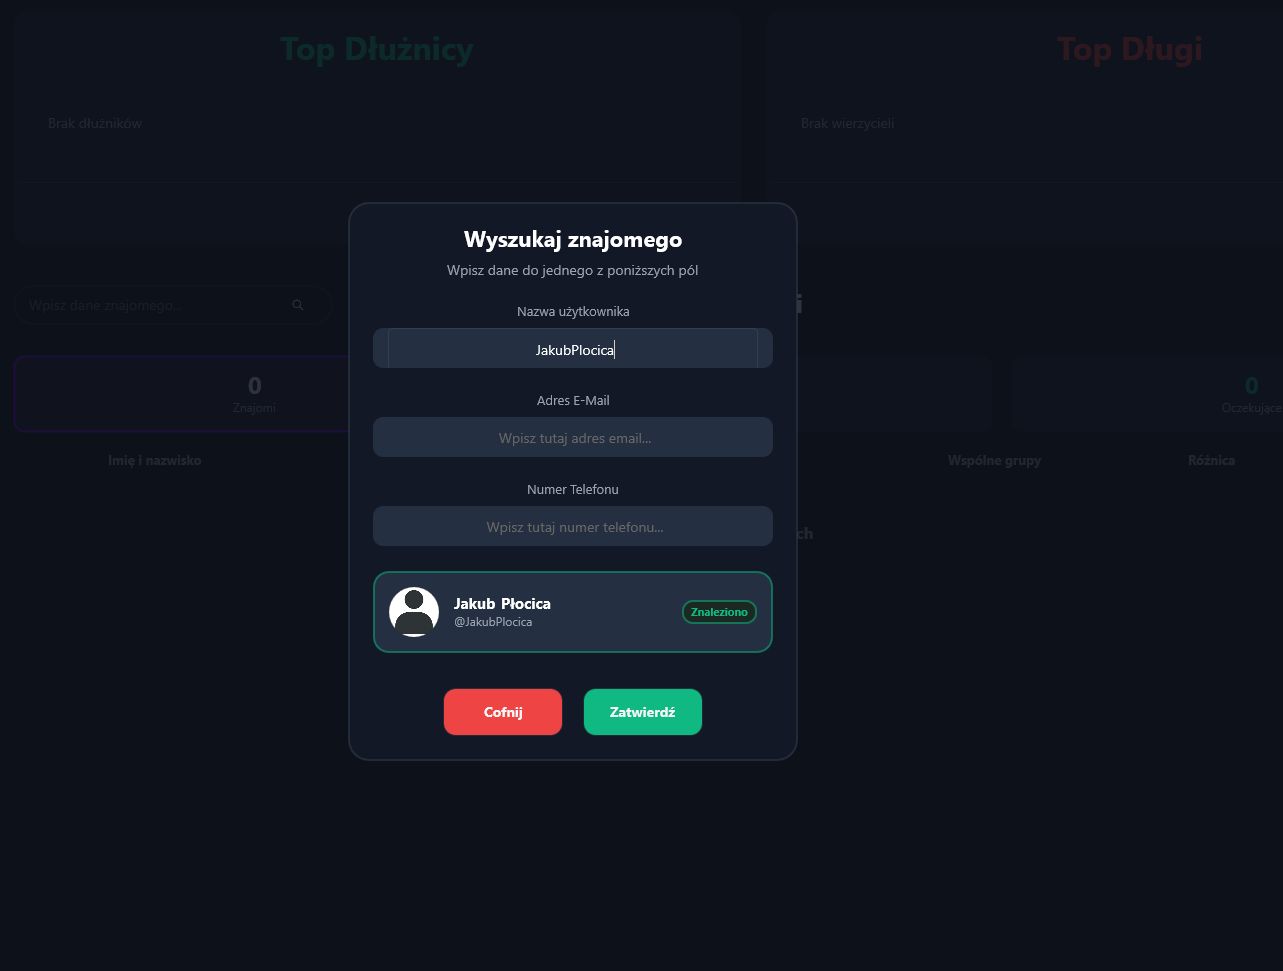
\includegraphics[width=0.95\textwidth]{img/friend/friend_wyszukiwanie.png}
    \vspace{0.5cm} \\
    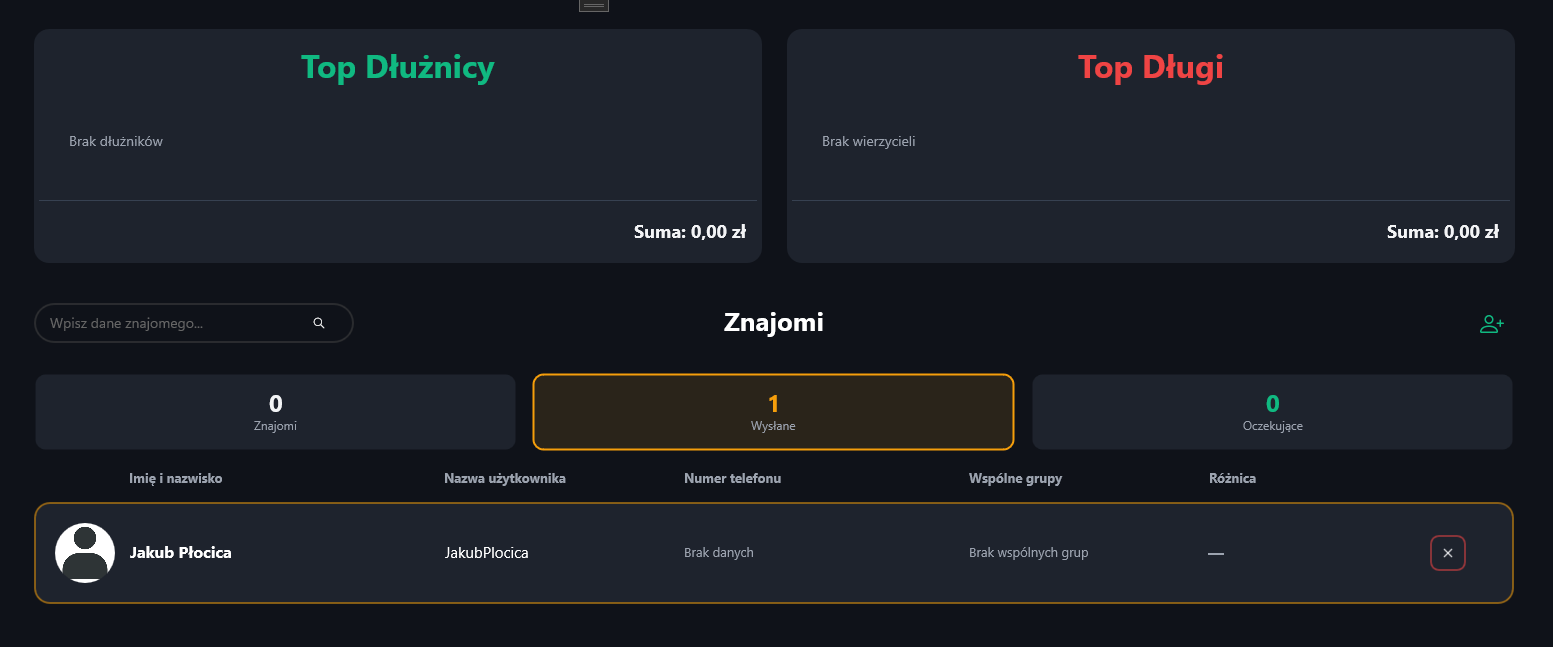
\includegraphics[width=0.95\textwidth]{img/friend/friend_wyslane_zaproszenia.png}
    \captionof{figure}{Inicjacja sieci kontaktów. Pusty stan modułu znajomych, silnik wyszukiwania użytkowników po predykatach (np. nazwa) oraz wgląd w zaproszenia oczekujące (Pending).}
\end{center}

\begin{center}
    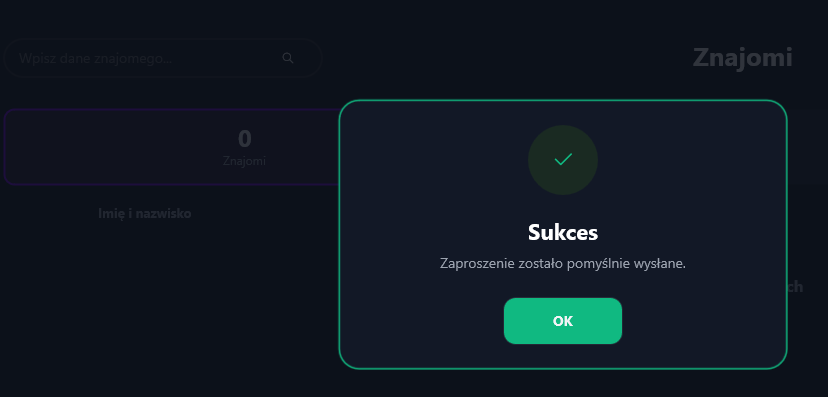
\includegraphics[width=0.95\textwidth]{img/friend/friend_success_zaproszenia.png}
    \vspace{0.5cm} \\
    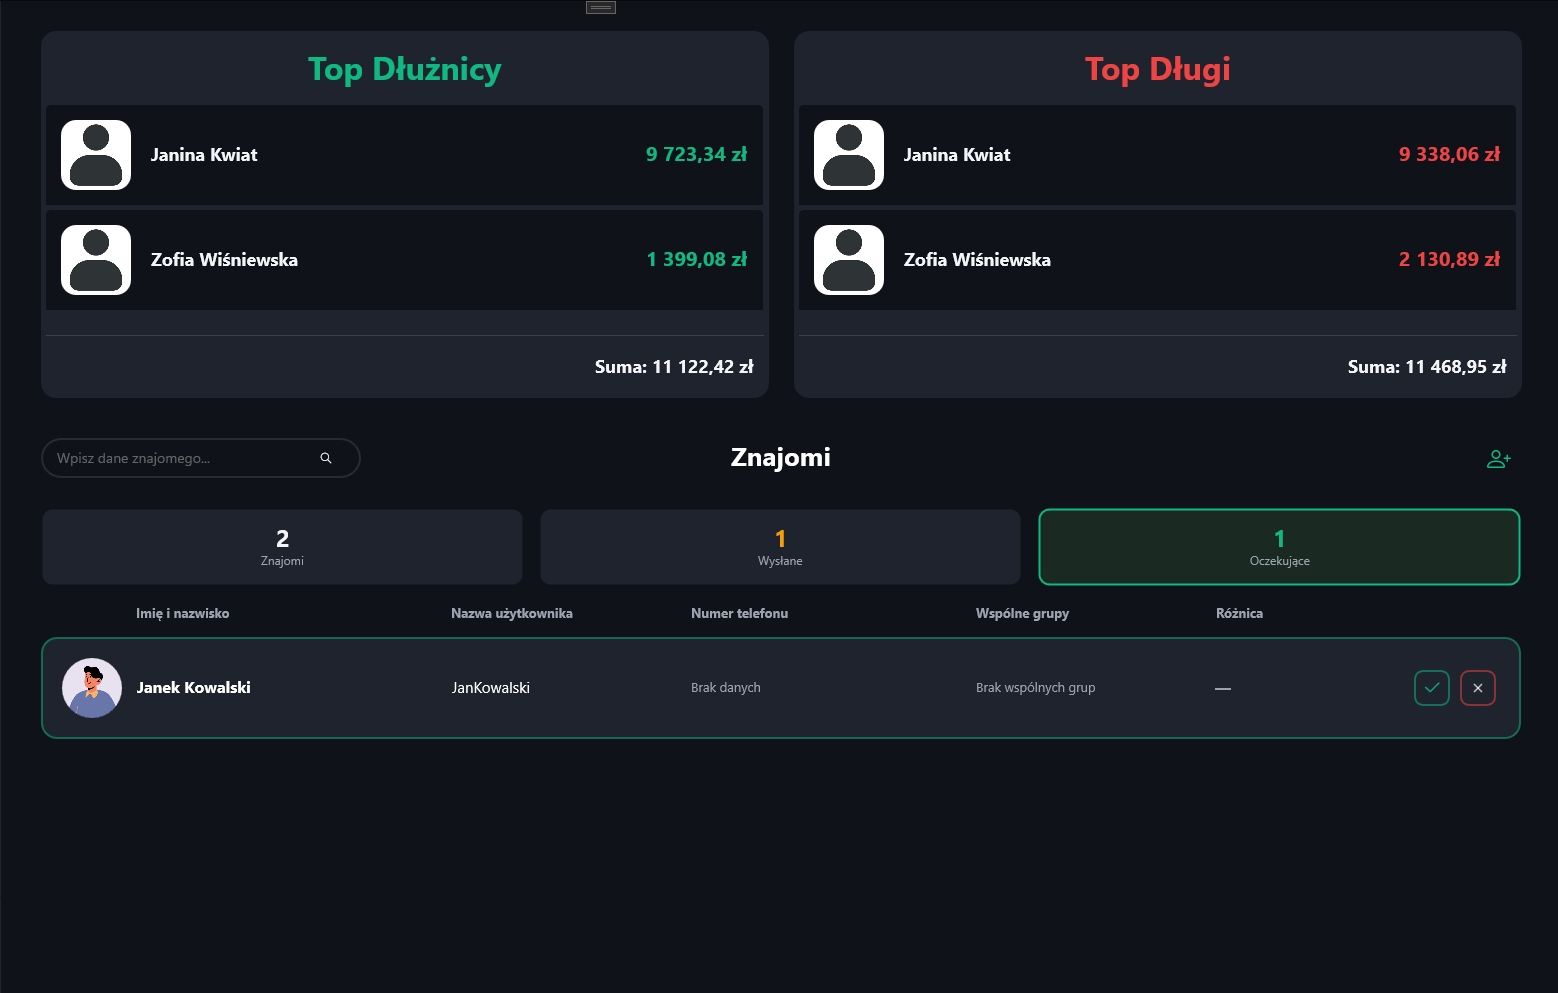
\includegraphics[width=0.95\textwidth]{img/friend/friend_oczekujace_zaproszenie.png}
    \vspace{0.5cm} \\
    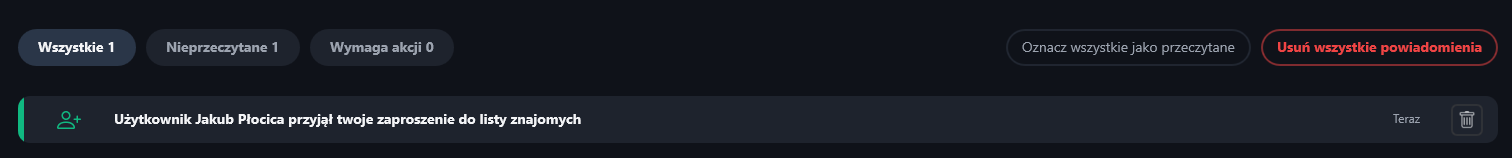
\includegraphics[width=0.95\textwidth]{img/friend/friend_powiadomienie_przyjecie.png}
    \captionof{figure}{Obsługa cyklu życia zaproszenia. Potwierdzenie wysłania, widok oczekującego zaproszenia u odbiorcy, i wygenerowanie notyfikacji w przypadku jego zaakceptowania.}
\end{center}

\begin{center}
    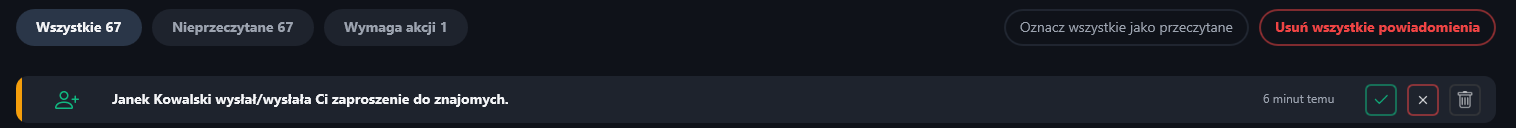
\includegraphics[width=0.95\textwidth]{img/friend/friend_powiadomienie_akceptacja.png}
    \vspace{0.5cm} \\
    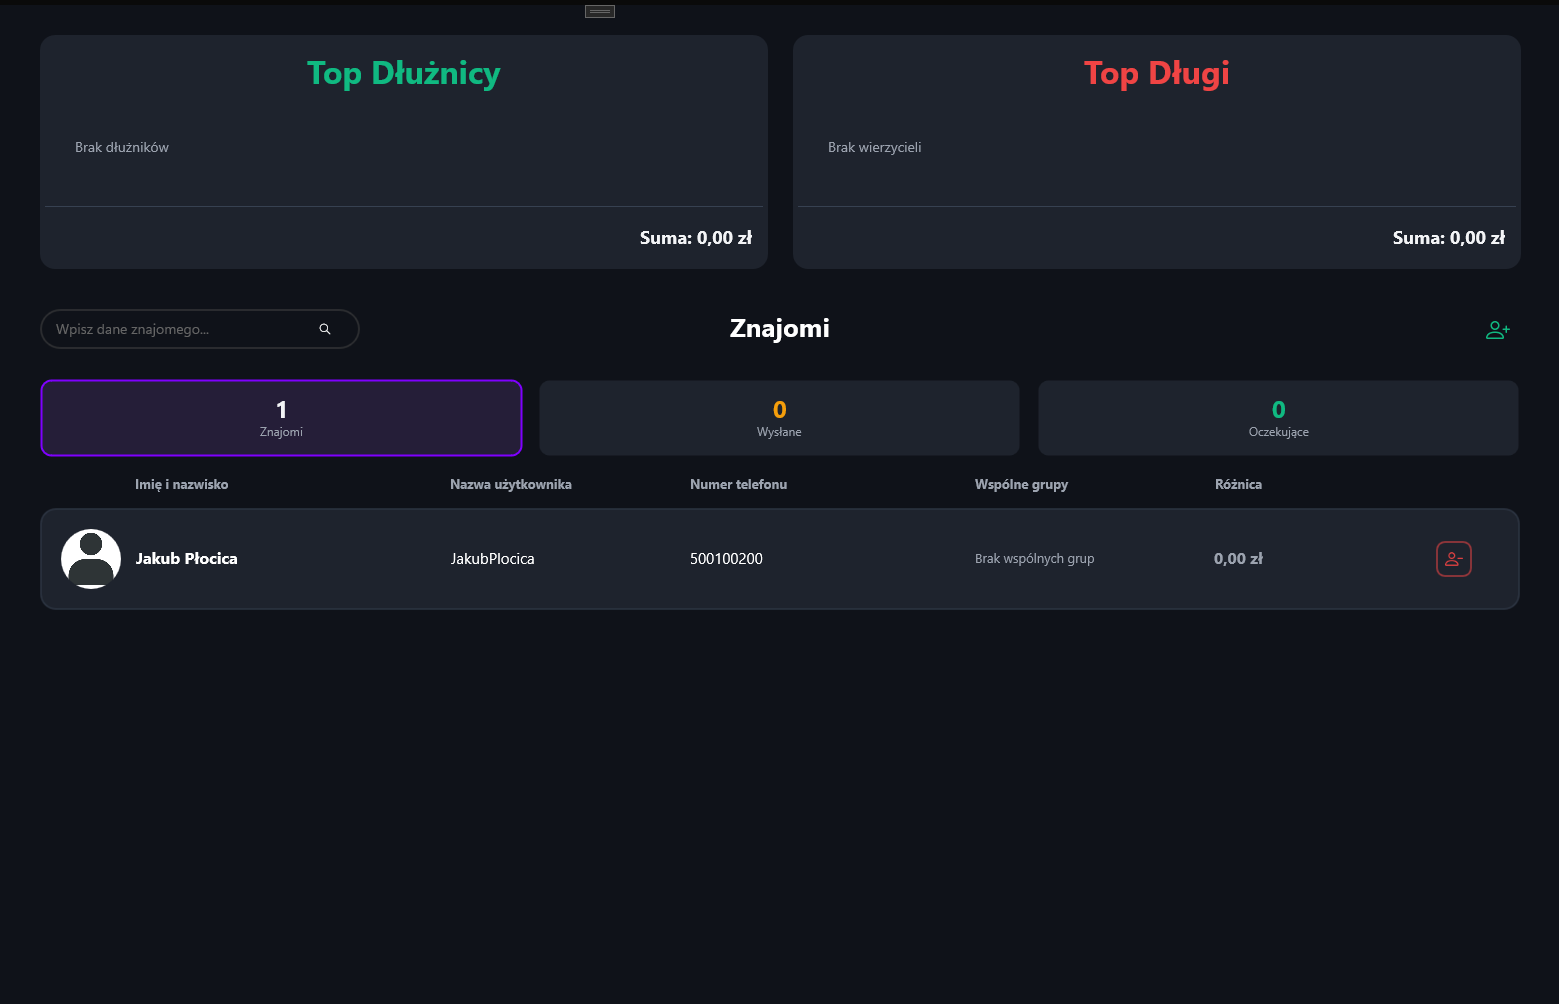
\includegraphics[width=0.95\textwidth]{img/friend/friend_nowy_widok_po_akceptacji.png}
    \captionof{figure}{Finalizacja nawiązania relacji. Odbiorca otrzymuje potwierdzenie z serwera, a widok znajomych zostaje odświeżony bez konieczności przeładowywania aplikacji.}
\end{center}

\begin{center}
    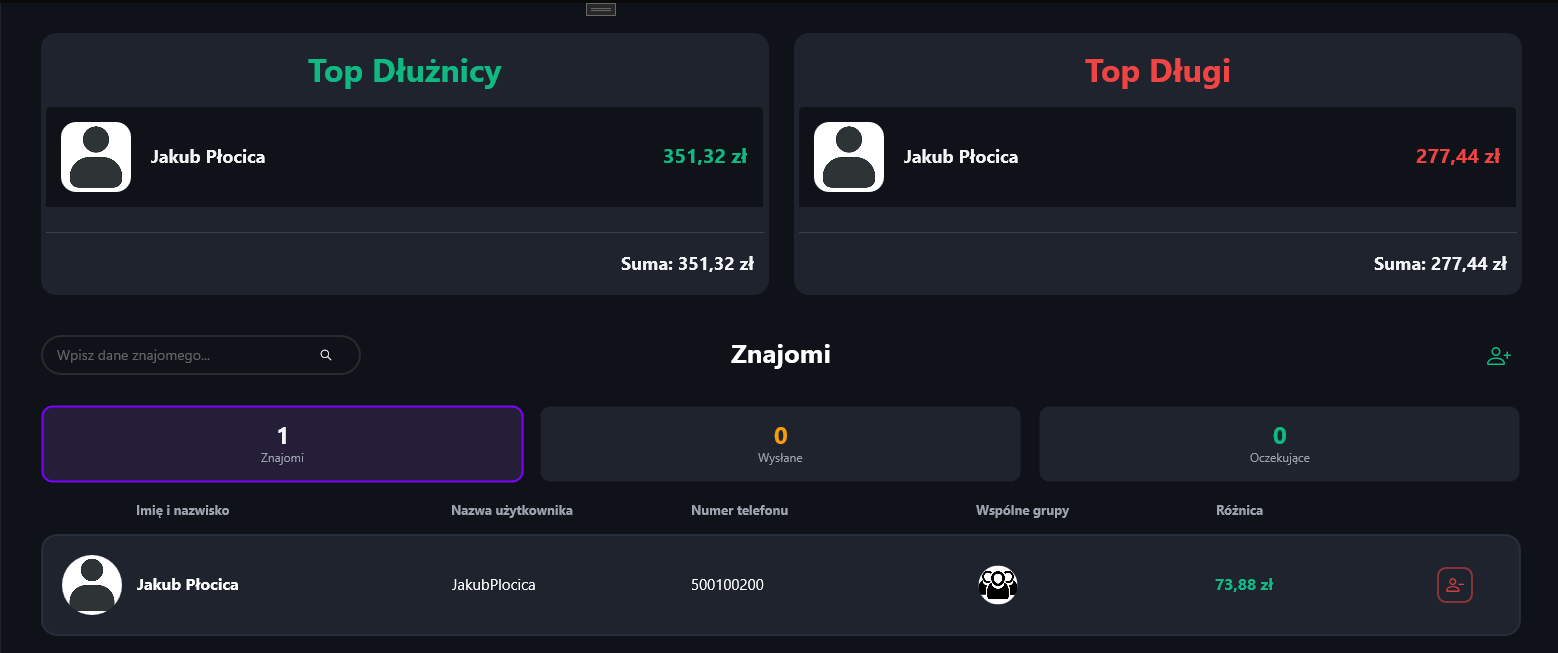
\includegraphics[width=0.95\textwidth]{img/friend/friend_ranking_po_dodaniu_wydatku.png}
    \captionof{figure}{Moduł grywalizacji / statystyk. Widoczny ranking powiązany ze znajomymi uwzględniający historię poniesionych wydatków po uprzednim ich zaksięgowaniu.}
\end{center}


\subsection{Krok 4: Tworzenie Ekosystemu (Grupy Wydatków)}
Po rozbudowaniu sieci kontaktów, tworzymy wspólne pokoje (Grupy). To w nich gromadzą się uczestnicy, zyskując uprawnienia (Admin/Member) i przypisując sobie role do późniejszego rozliczania.

\begin{center}
    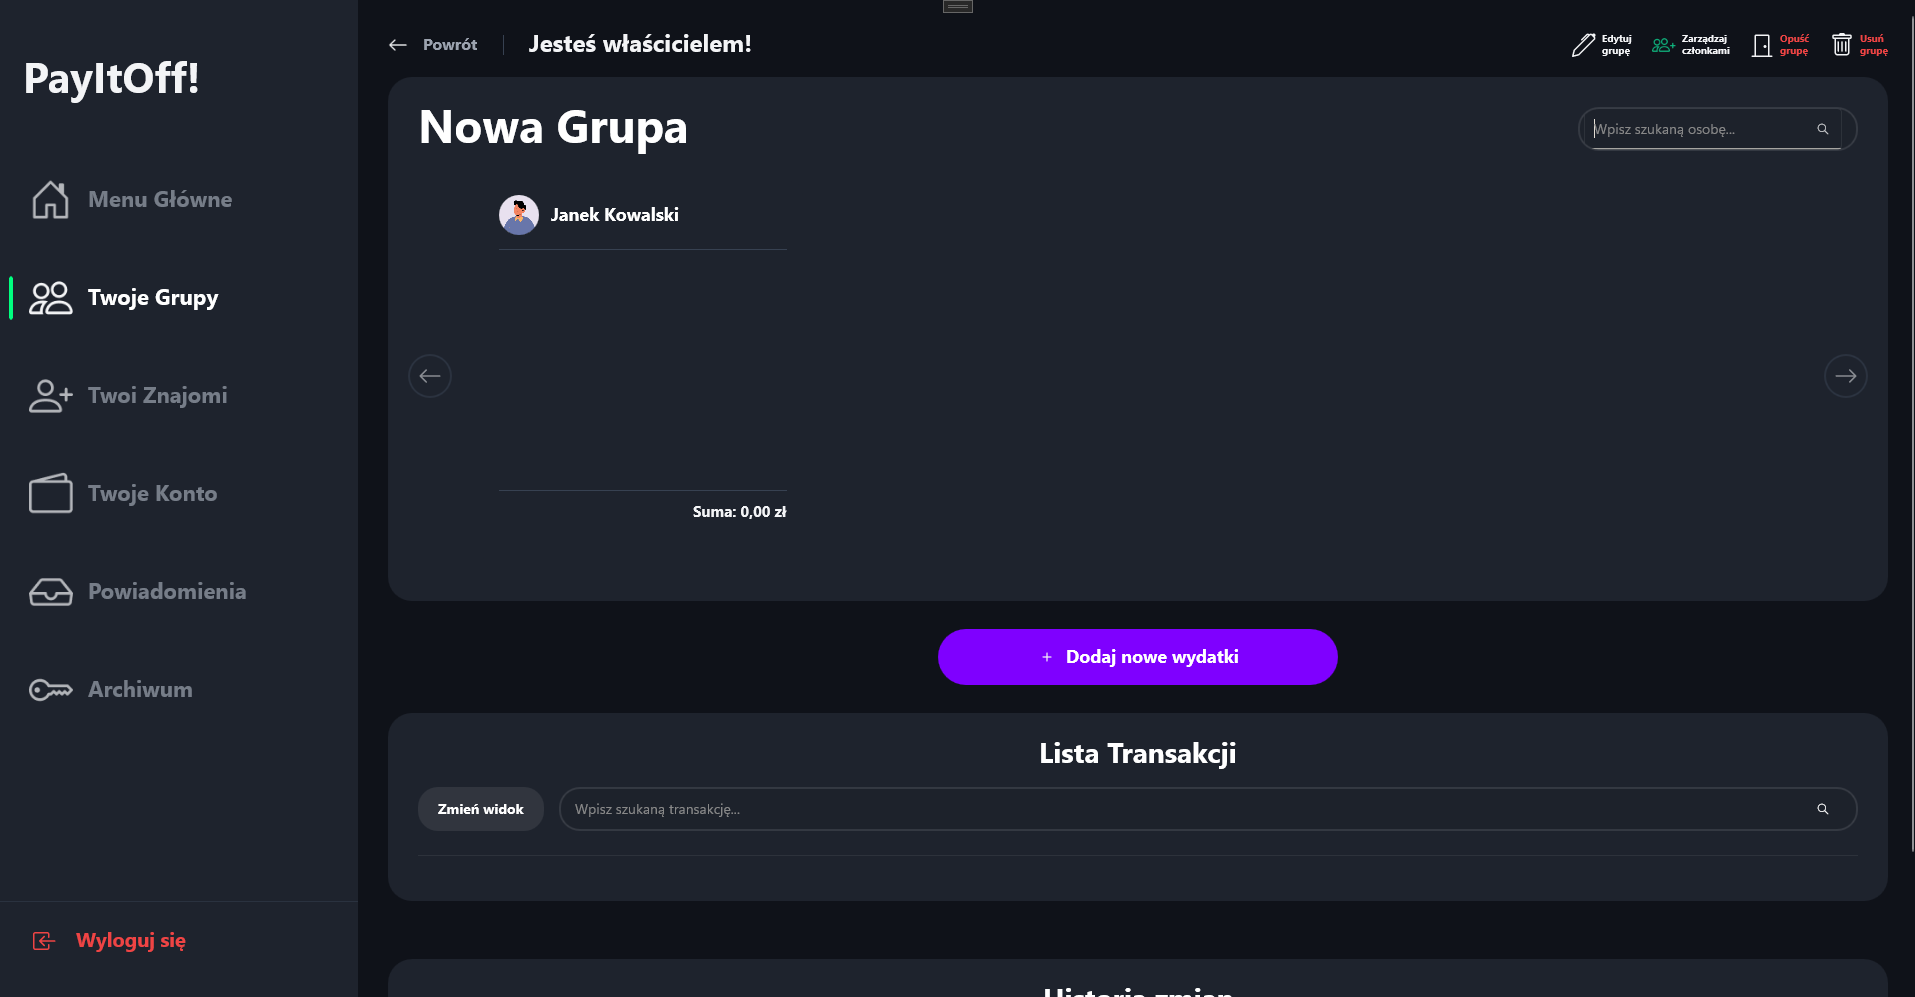
\includegraphics[width=0.95\textwidth]{img/group/group_pusty_widok.png}
    \vspace{0.5cm} \\
    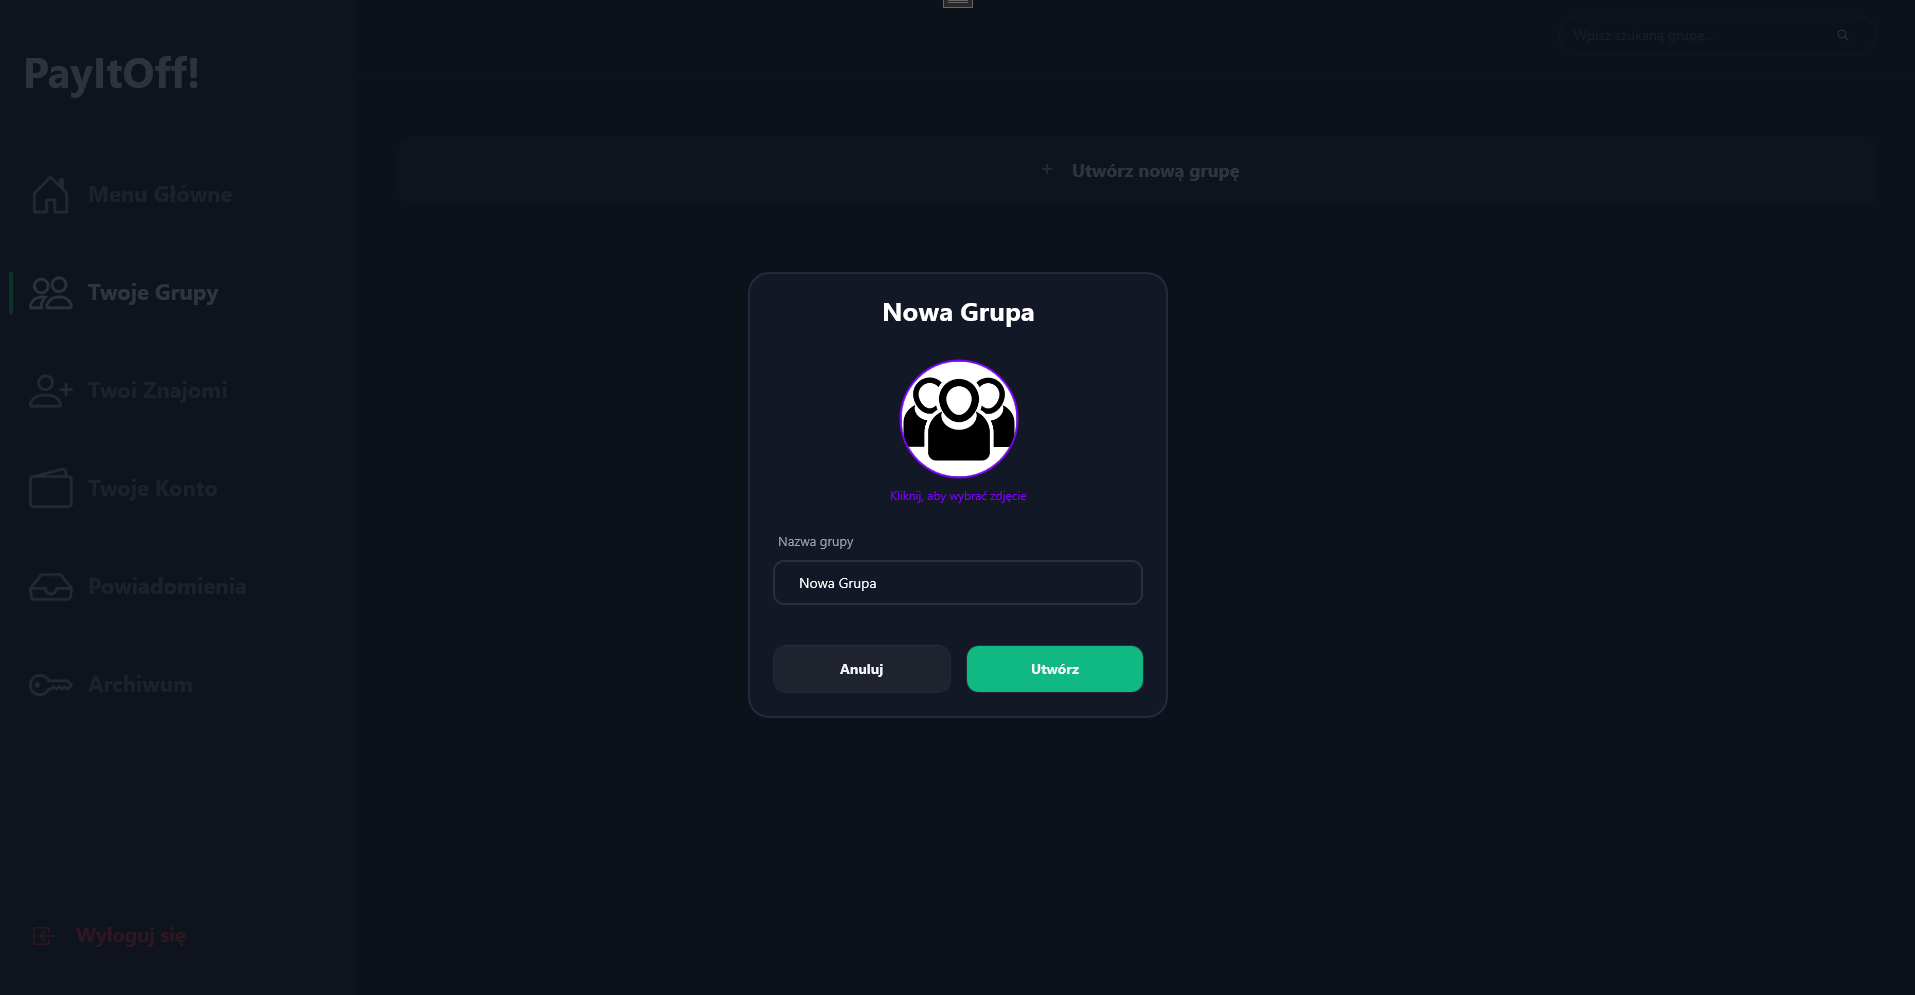
\includegraphics[width=0.95\textwidth]{img/group/group_tworzenie.png}
    \captionof{figure}{Inicjacja grupy rozliczeniowej. Po lewej ekran startowy, po prawej formularz tworzenia nowego środowiska współdzielonego z przypisywaniem nazwy.}
\end{center}

\begin{center}
    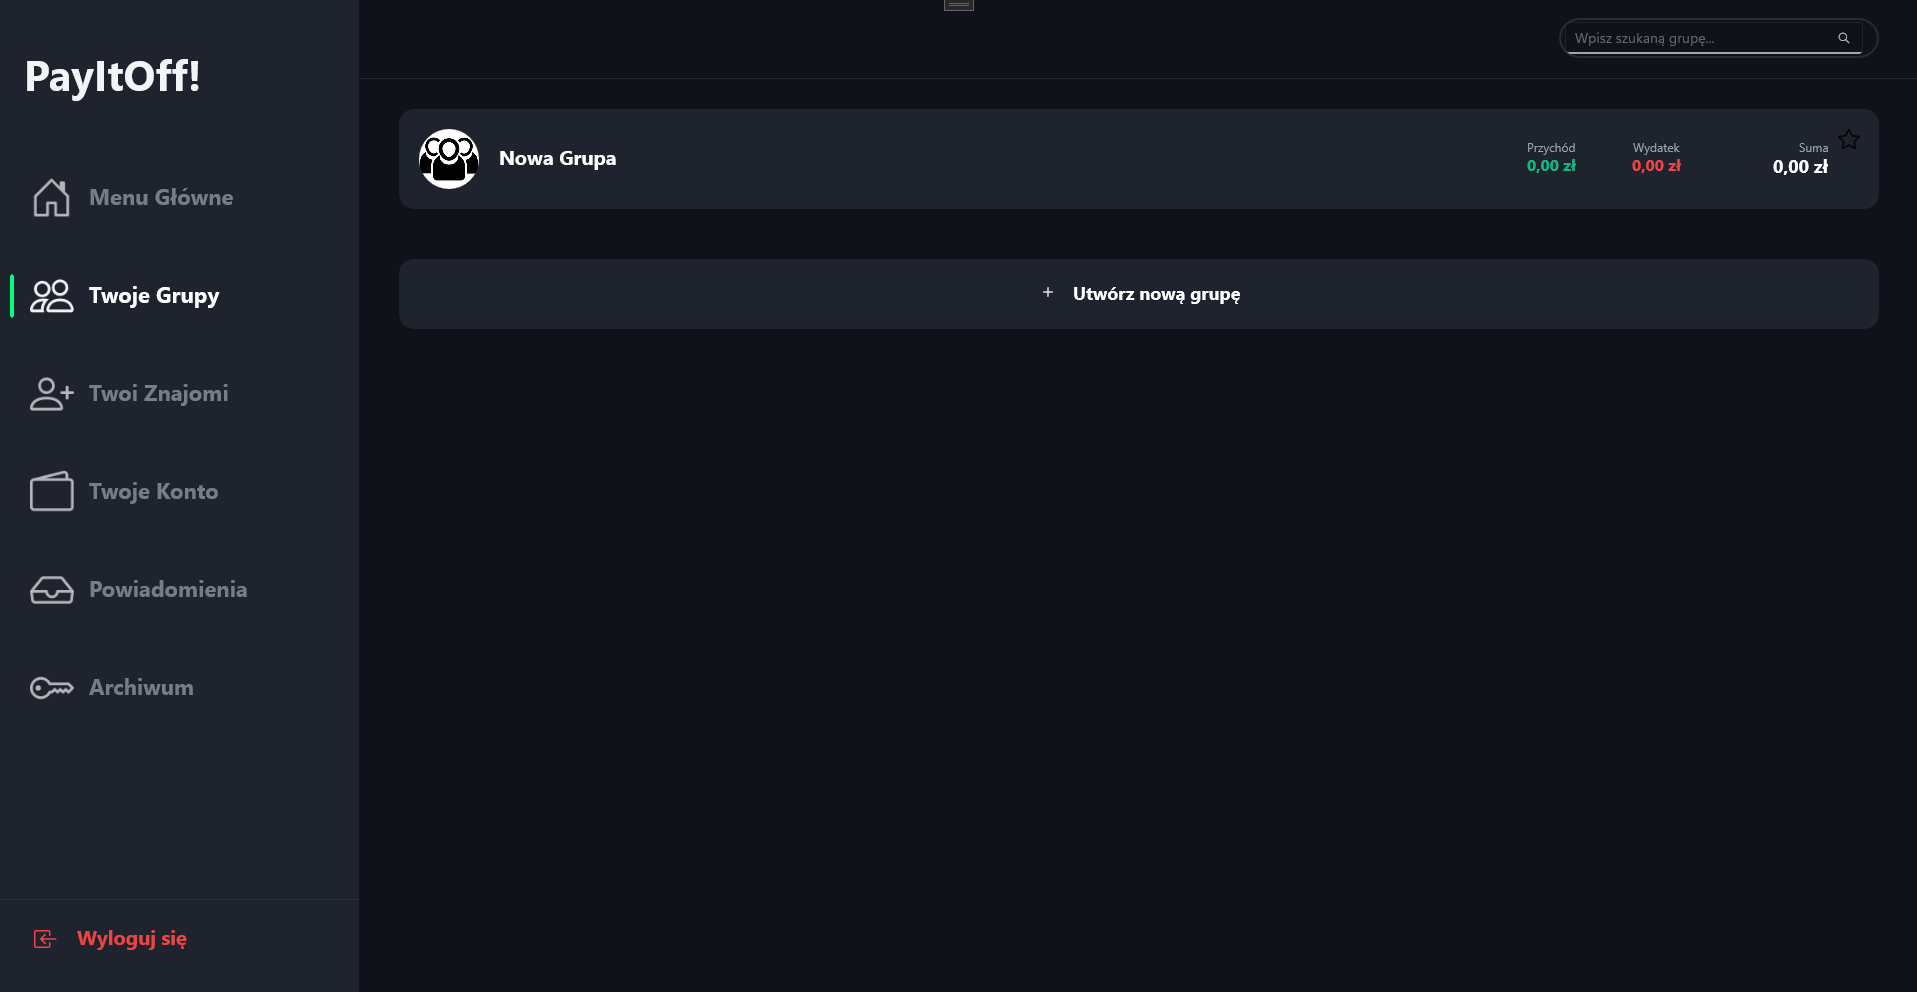
\includegraphics[width=0.95\textwidth]{img/group/group_utworzona_grupa.png}
    \vspace{0.5cm} \\
    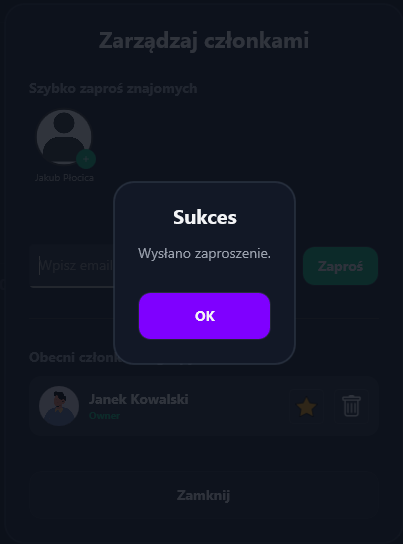
\includegraphics[width=0.45\textwidth]{img/group/group_szybkie_zaproszenie_znajomego.png}
    \captionof{figure}{Widok nowo powstałej grupy oraz wykorzystanie dedykowanego modułu szybkiego zapraszania znajomych do współpracy.}
\end{center}

\begin{center}
    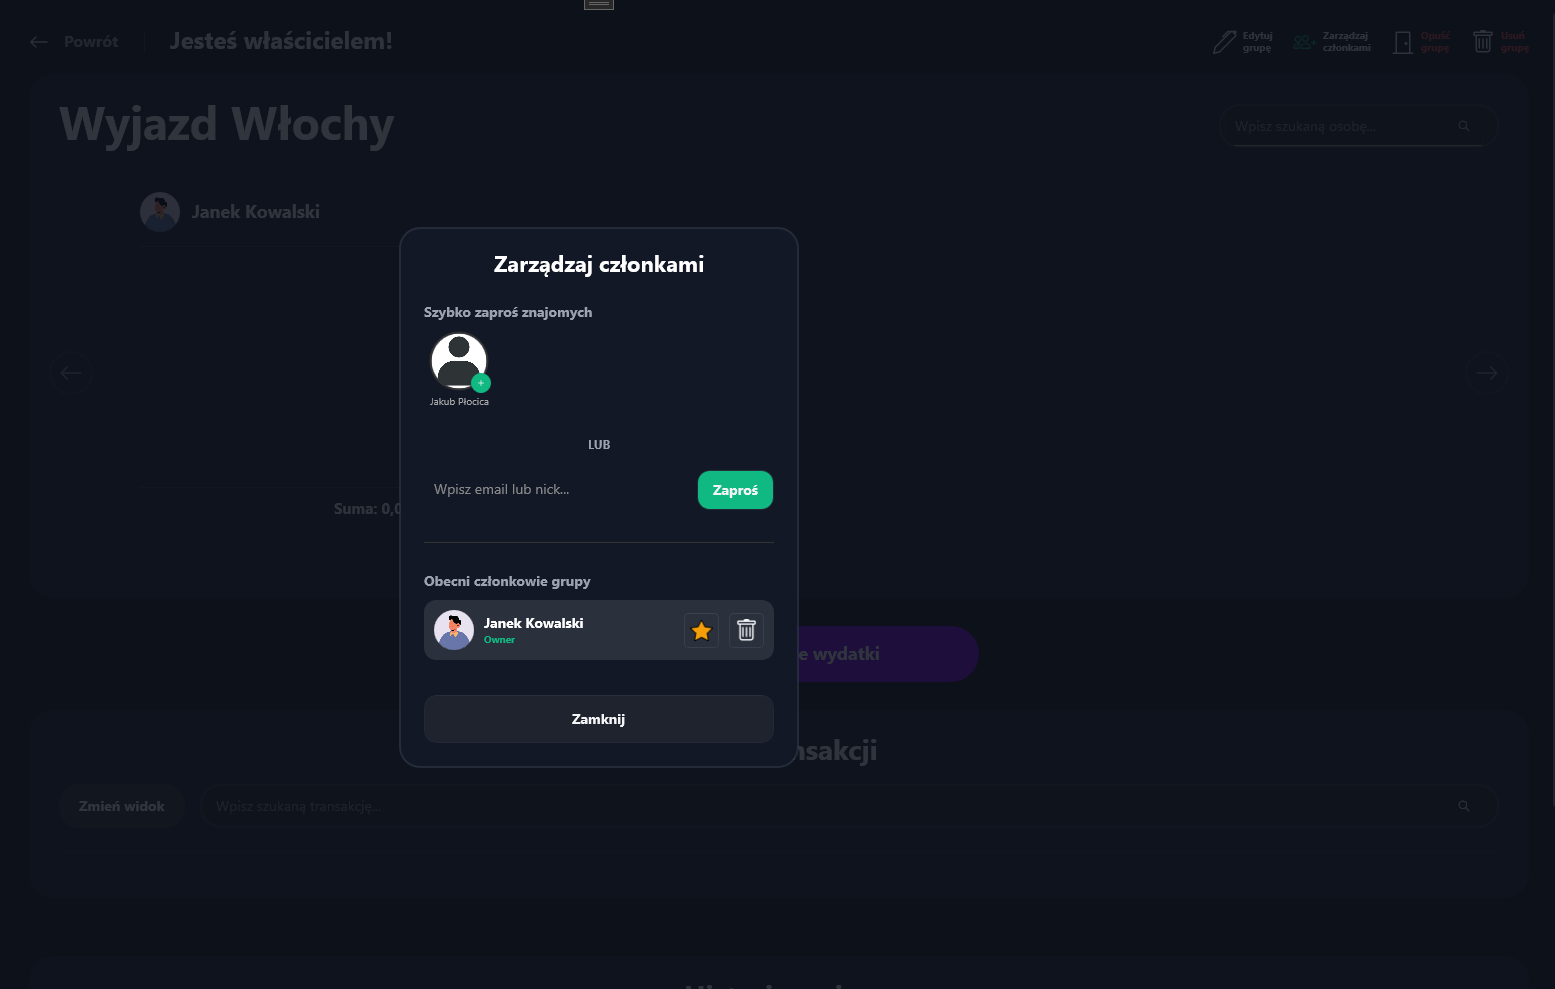
\includegraphics[width=0.95\textwidth]{img/group/group_zaproszenie_członkow.png}
    \vspace{0.5cm} \\
    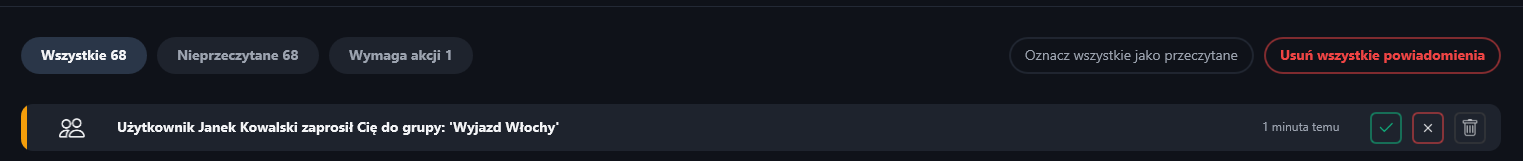
\includegraphics[width=0.95\textwidth]{img/group/group_powiadomienie_zaproszenia.png}
    \vspace{0.5cm} \\
    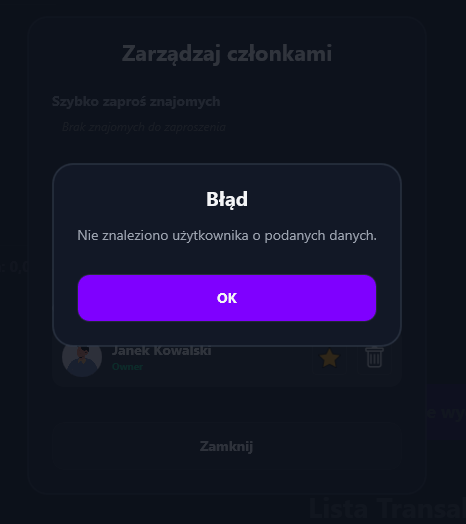
\includegraphics[width=0.45\textwidth]{img/group/group_bledny_nick_zaproszenia.png}
    \captionof{figure}{Zarządzanie członkostwem. Ręczne wpisywanie identyfikatora, notyfikacja o nowym zaproszeniu na urządzeniu docelowym oraz ścisła obsługa błędu nieistniejącego użytkownika.}
\end{center}

\begin{center}
    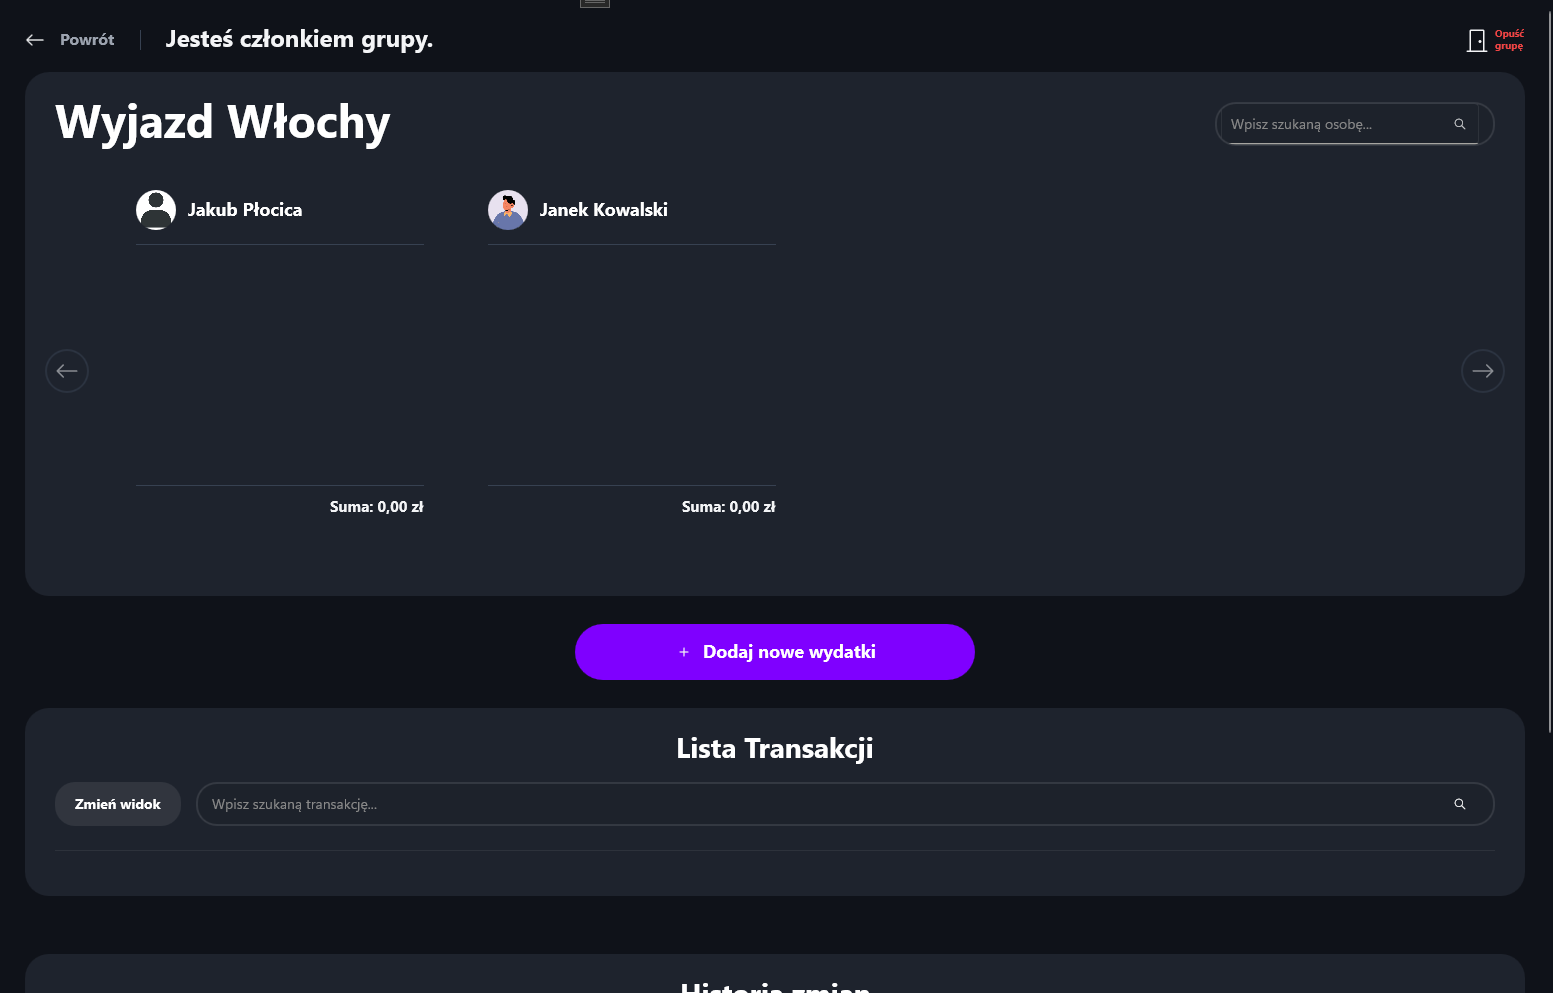
\includegraphics[width=0.95\textwidth]{img/group/group_widok_czlonka.png}
    \vspace{0.5cm} \\
    
\includegraphics[width=0.45\textwidth]{img/group/group_zmiana_nazwy.png}
    \hfill
    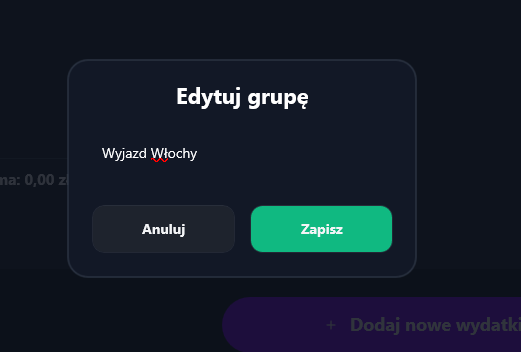
\includegraphics[width=0.45\textwidth]{img/group/group_edycja_nazwy.png}
    \captionof{figure}{Panel administracyjny. Kontrola nad uprawnieniami przypisanymi do członków (RBAC) oraz dostęp do płynnej edycji metadanych grupy (np. nazwy).}
\end{center}

\begin{center}
    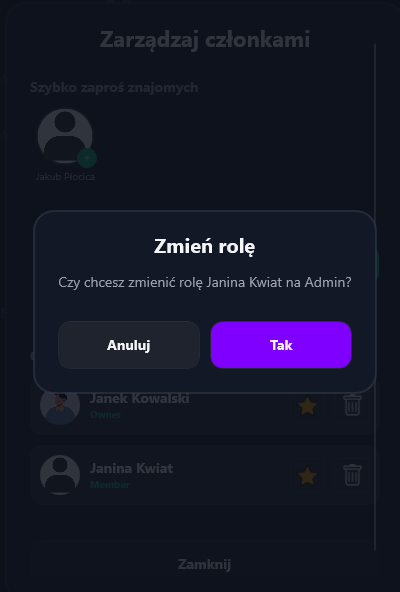
\includegraphics[width=0.45\textwidth]{img/group/group_zmiana_roli_admin.png}
    \vspace{0.5cm} \\
    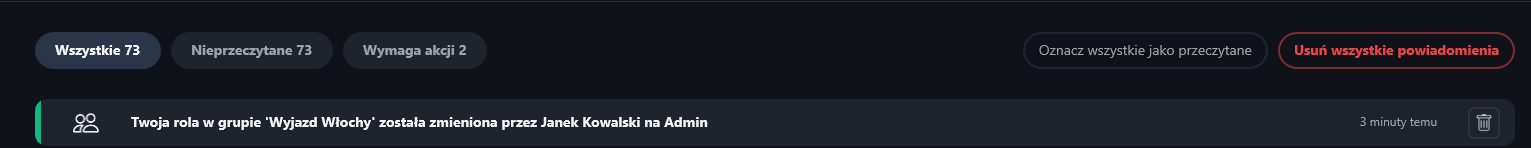
\includegraphics[width=0.95\textwidth]{img/group/group_powiadomienie_zmiana_roli.png}
    \vspace{0.5cm} \\
    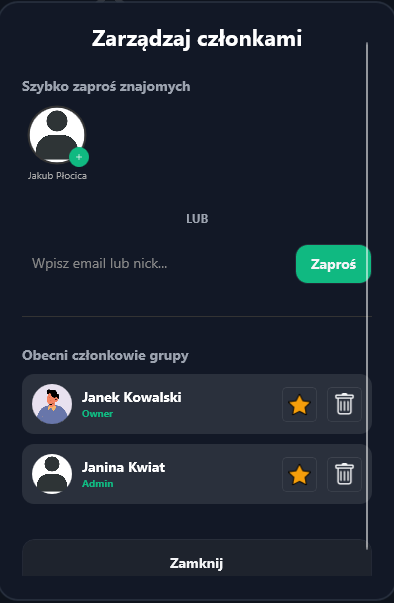
\includegraphics[width=0.45\textwidth]{img/group/group_udana_zmiana_roli.png}
    \captionof{figure}{Zarządzanie uprawnieniami. Przekazanie roli administratora innemu użytkownikowi, odebranie powiadomienia w czasie rzeczywistym i ostateczny widok odświeżonego statusu.}
\end{center}

\begin{center}
    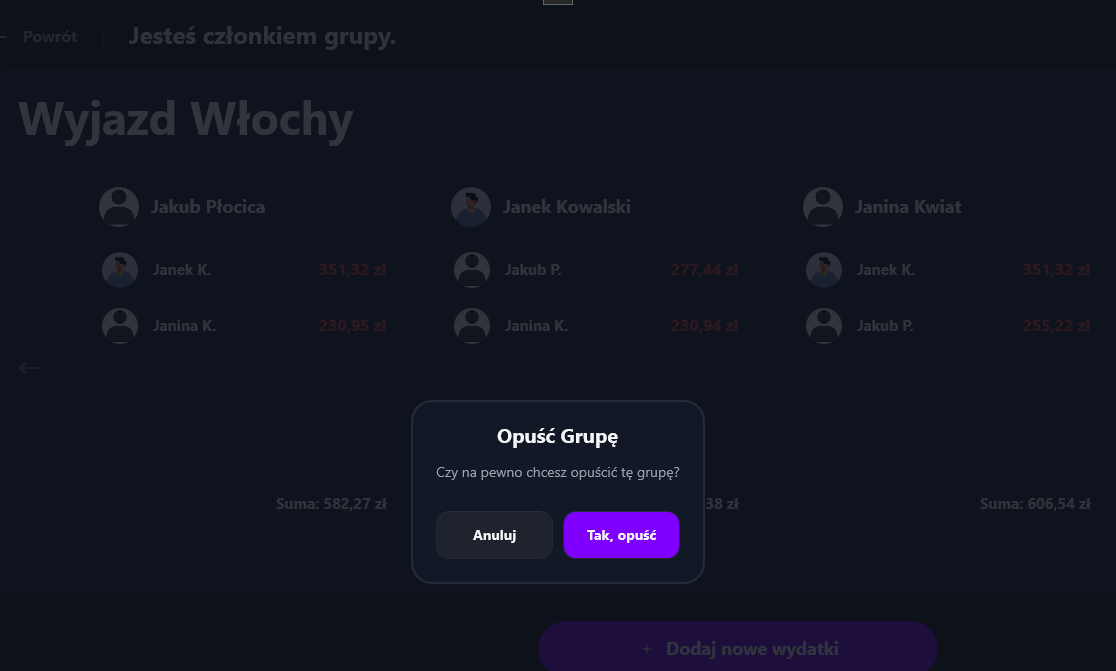
\includegraphics[width=0.95\textwidth]{img/group/group_opuszczenie_grupy.png}
    \vspace{0.5cm} \\
    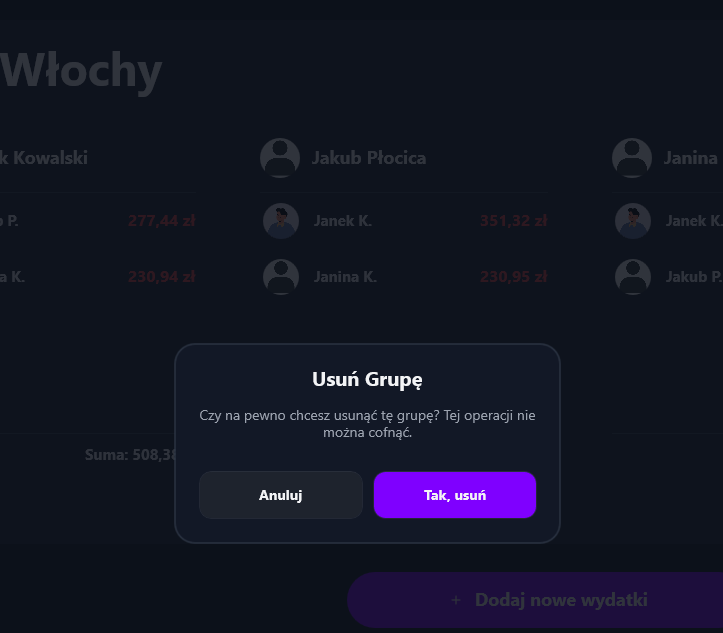
\includegraphics[width=0.45\textwidth]{img/group/group_usuniecie_grupy.png}
    \captionof{figure}{Ostatnie fazy istnienia użytkownika lub grupy. Proces bezpiecznego opuszczenia (wymaga spłaty długów) oraz panel trwałego usuwania całego środowiska.}
\end{center}


\subsection{Krok 5: Księgowanie Rachunków (Wydatki)}
Kluczowy etap, gdzie na podstawie zrobionych zakupów dodajemy konkretne paragony. System pozwala kategoryzować wydatki, używać parsera matematycznego w locie i dynamicznie ustalać udziały procentowe/ułamkowe z zabezpieczeniem przed błędem reszty (Penny-Drop problem).

\begin{center}
    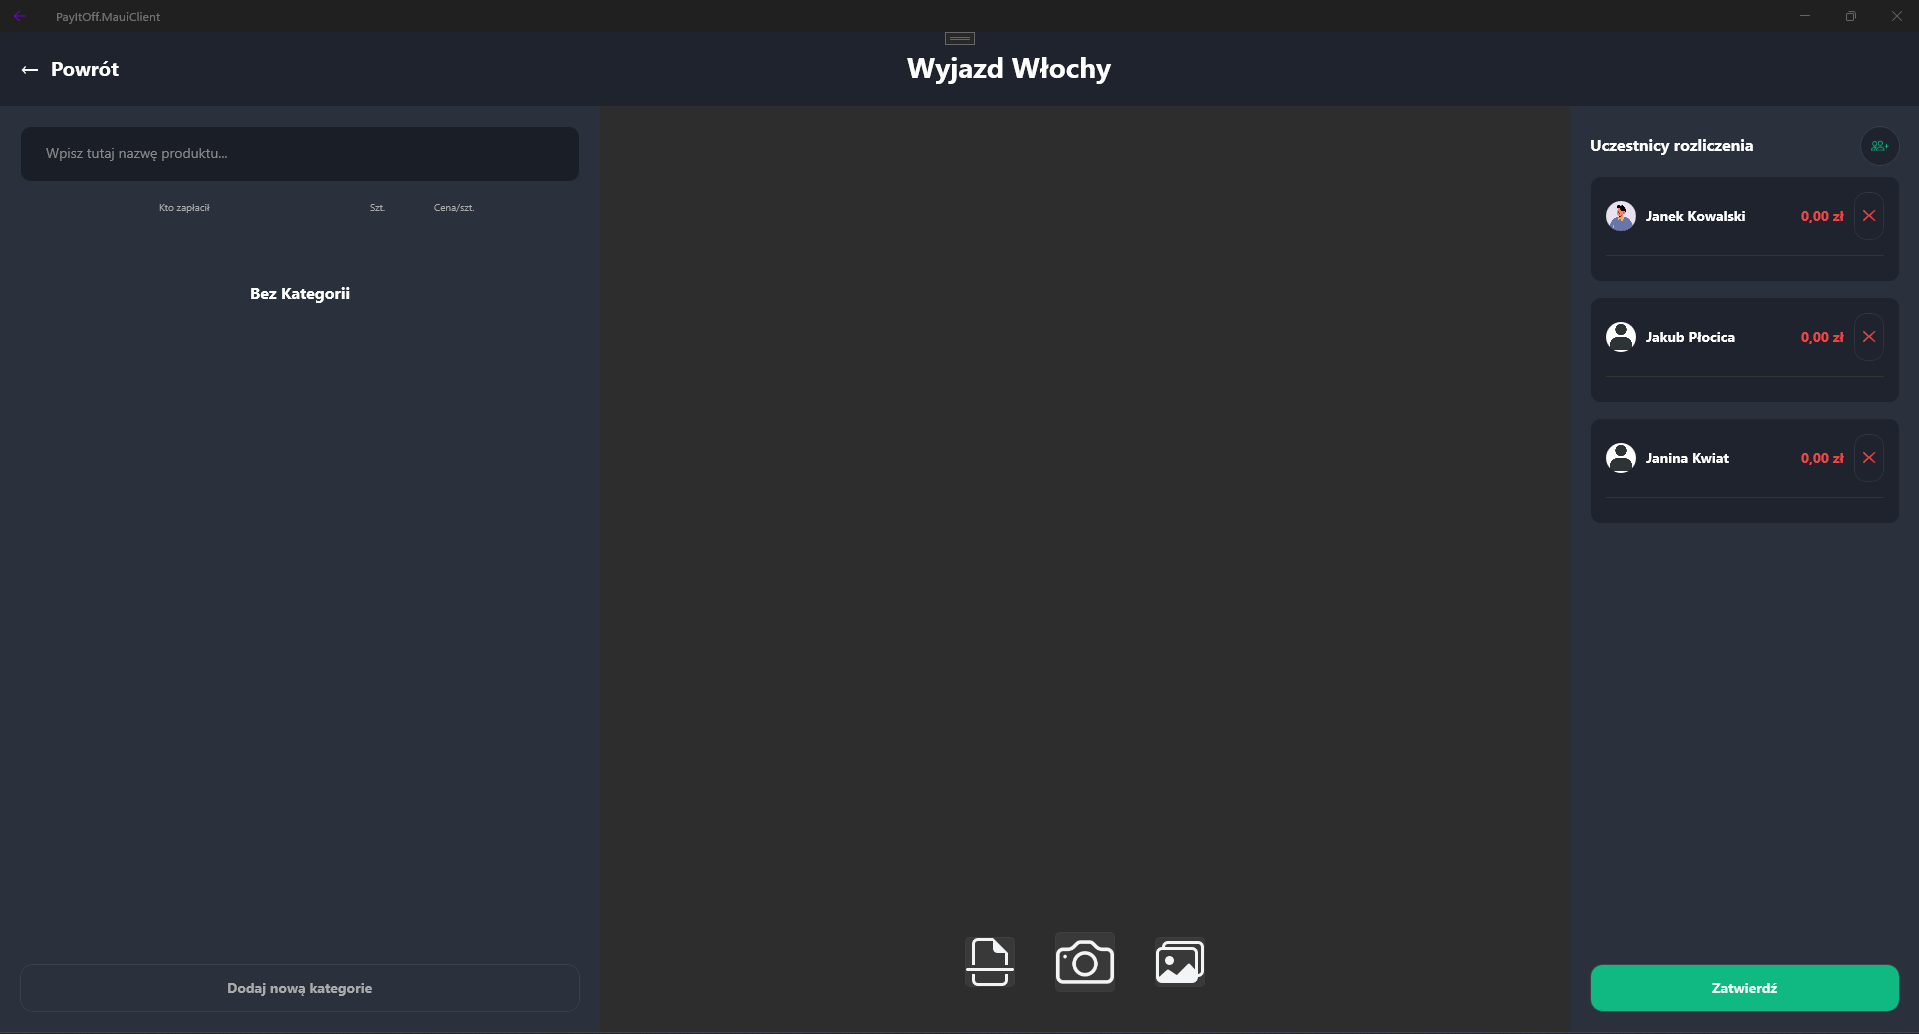
\includegraphics[width=0.95\textwidth]{img/new_expense/expense_pusty.png}
    \vspace{0.5cm} \\
    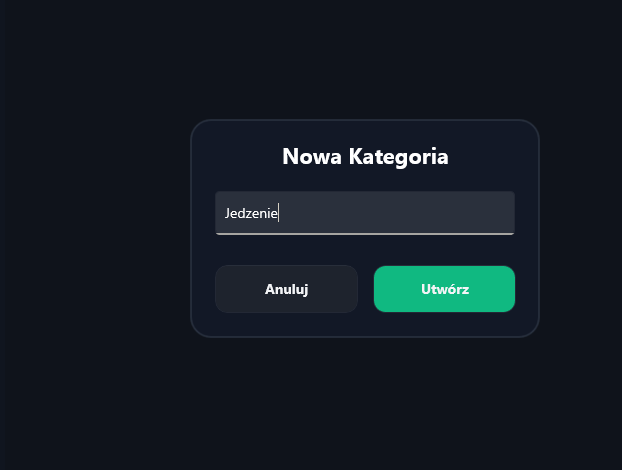
\includegraphics[width=0.45\textwidth]{img/new_expense/new_expense_stworzenie_kategorii.png}
    \captionof{figure}{Stan początkowy zakładki wydatków w nowej grupie oraz kreator własnych kategorii wydatkowych pomagający w analityce i utrzymaniu porządku.}
\end{center}

\begin{center}
    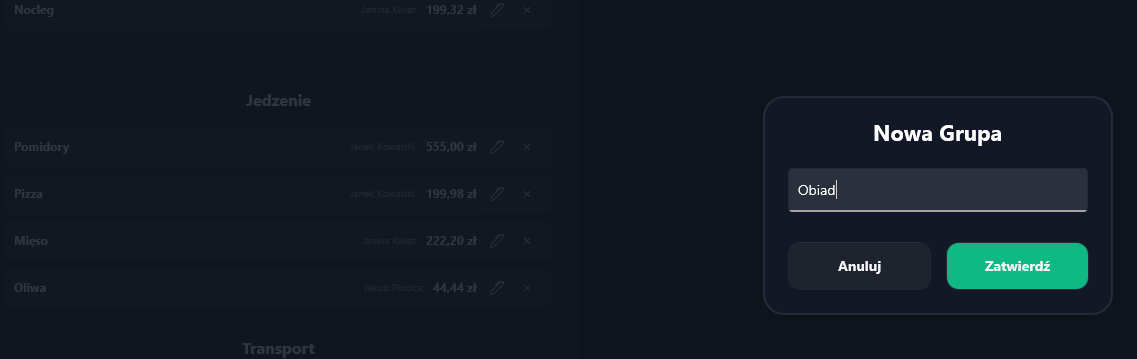
\includegraphics[width=0.95\textwidth]{img/new_expense/new_expense_stworzenie_grupy_produktow.png}
    \vspace{0.5cm} \\
    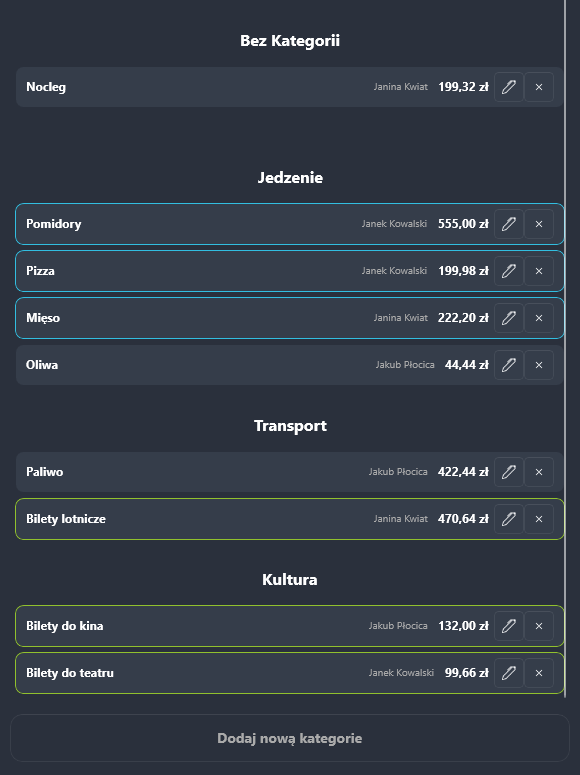
\includegraphics[width=0.45\textwidth]{img/new_expense/new_expense_przypisane_kategorii_oraz_grup.png}
    \vspace{0.5cm} \\
    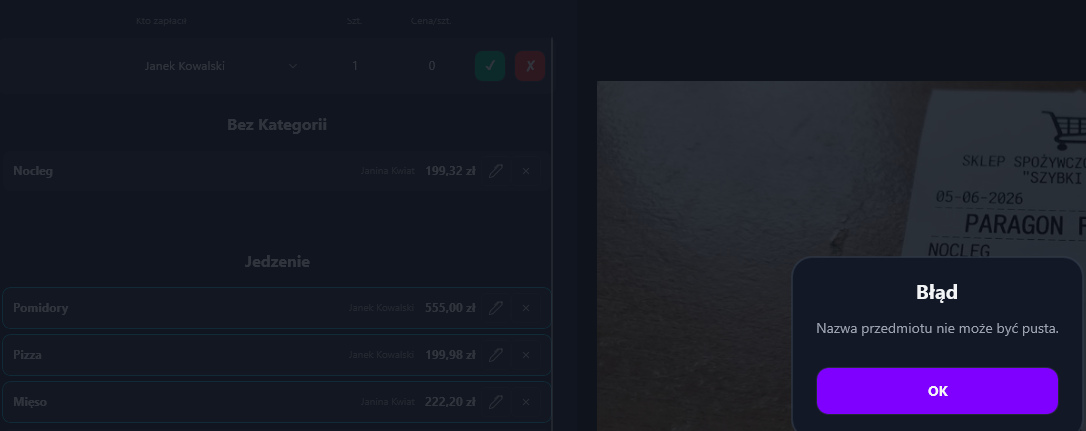
\includegraphics[width=0.95\textwidth]{img/new_expense/new_expense_proba_dodanie_przedmiotu_bez_nazwy.png}
    \captionof{figure}{Grupowanie pojedynczych produktów paragonu. Przypisywanie tagów oraz restrykcyjna walidacja po stronie klienta (zapobieganie pustym nazwom pozycji).}
\end{center}

\begin{center}
    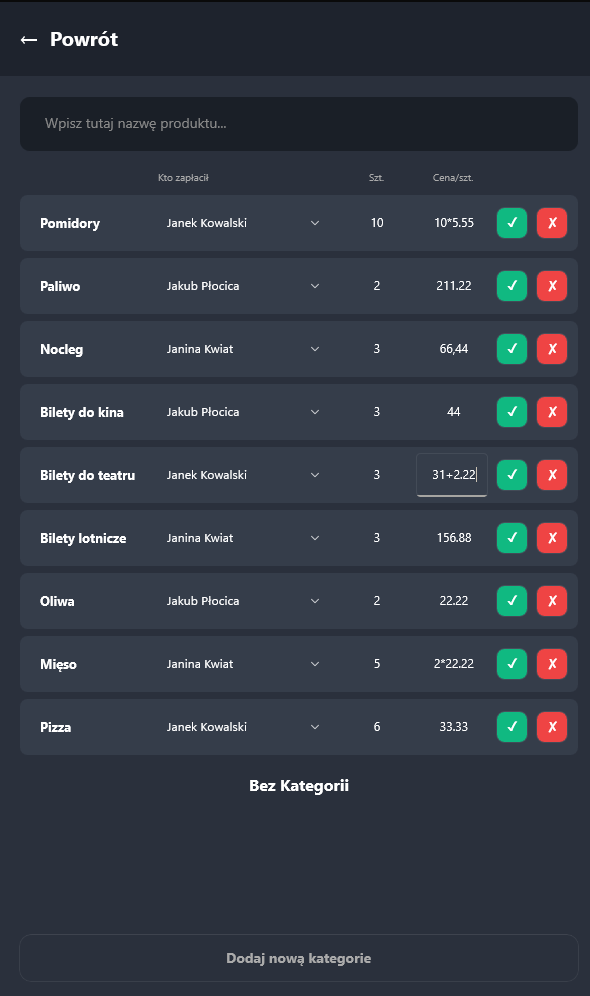
\includegraphics[width=0.45\textwidth]{img/new_expense/new_expense_wpisane_przedmioty_przydzieleni_wiezyciele_operacje_matematyczne.png}
    \hfill
    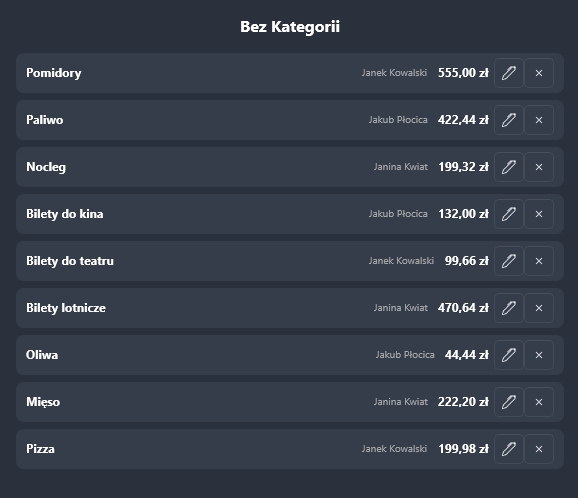
\includegraphics[width=0.45\textwidth]{img/new_expense/new_expense_zatwierdzenie_przedmiotow.png}
    \captionof{figure}{Innowacyjne użycie parsera matematycznego (np. wpisanie 10+5 w polu ceny) i elastyczne przydzielanie dłużników do konkretnych pozycji na rachunku.}
\end{center}

\begin{center}
    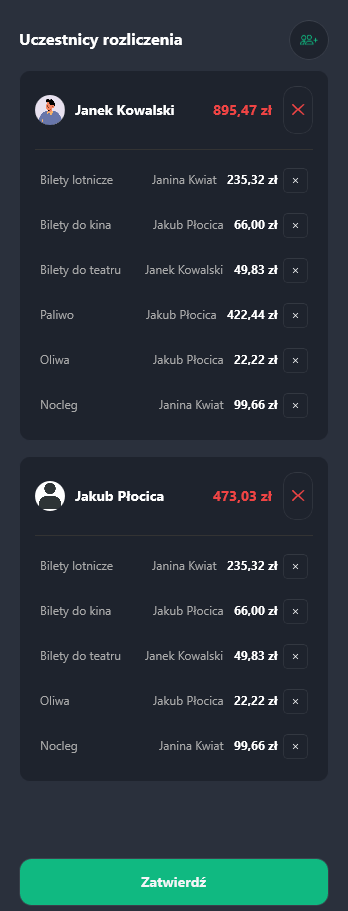
\includegraphics[width=0.45\textwidth]{img/new_expense/new_expense_usuniecie_uczestnika_zmiana_kwot.png}
    \hfill
    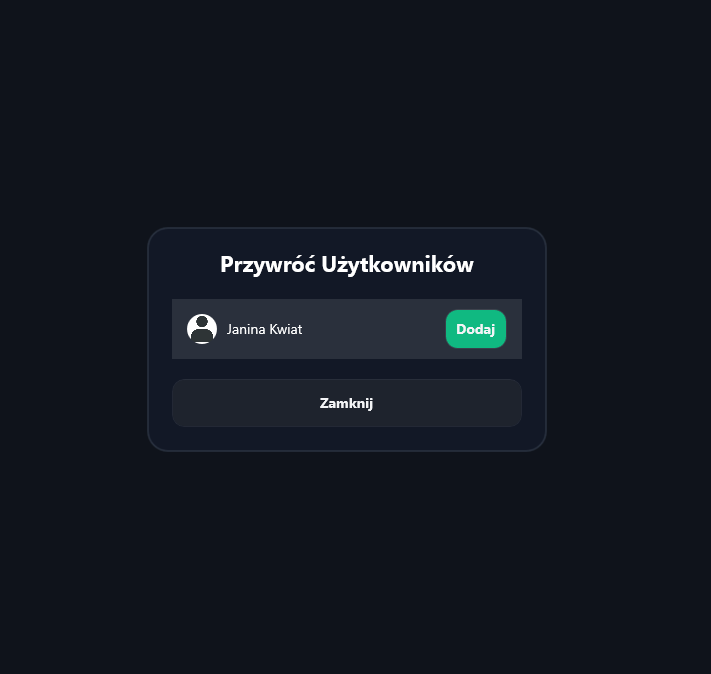
\includegraphics[width=0.45\textwidth]{img/new_expense/new_expense_przywracanie.png}
    \vspace{0.5cm} \\
    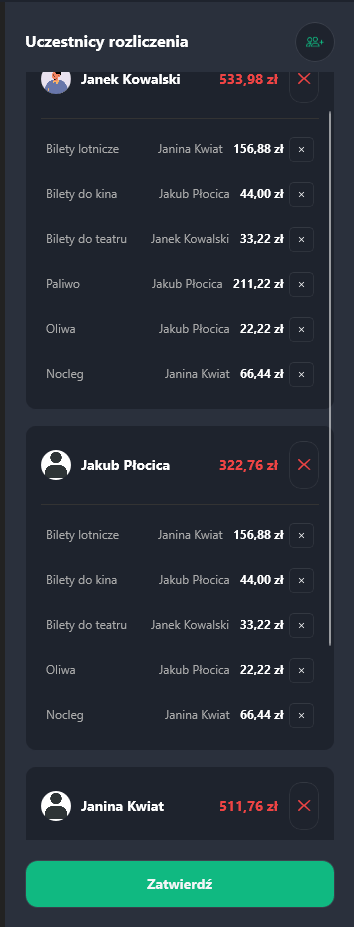
\includegraphics[width=0.45\textwidth]{img/new_expense/new_expense_podzial_wydatkow.png}
    \captionof{figure}{Silnik kalkulacji udziałów. Reaktywne przeliczanie obciążeń finansowych po usunięciu/przywróceniu płatnika. Dostęp do zaawansowanych algorytmów podziału procentowego i równomiernego.}
\end{center}

\begin{center}
    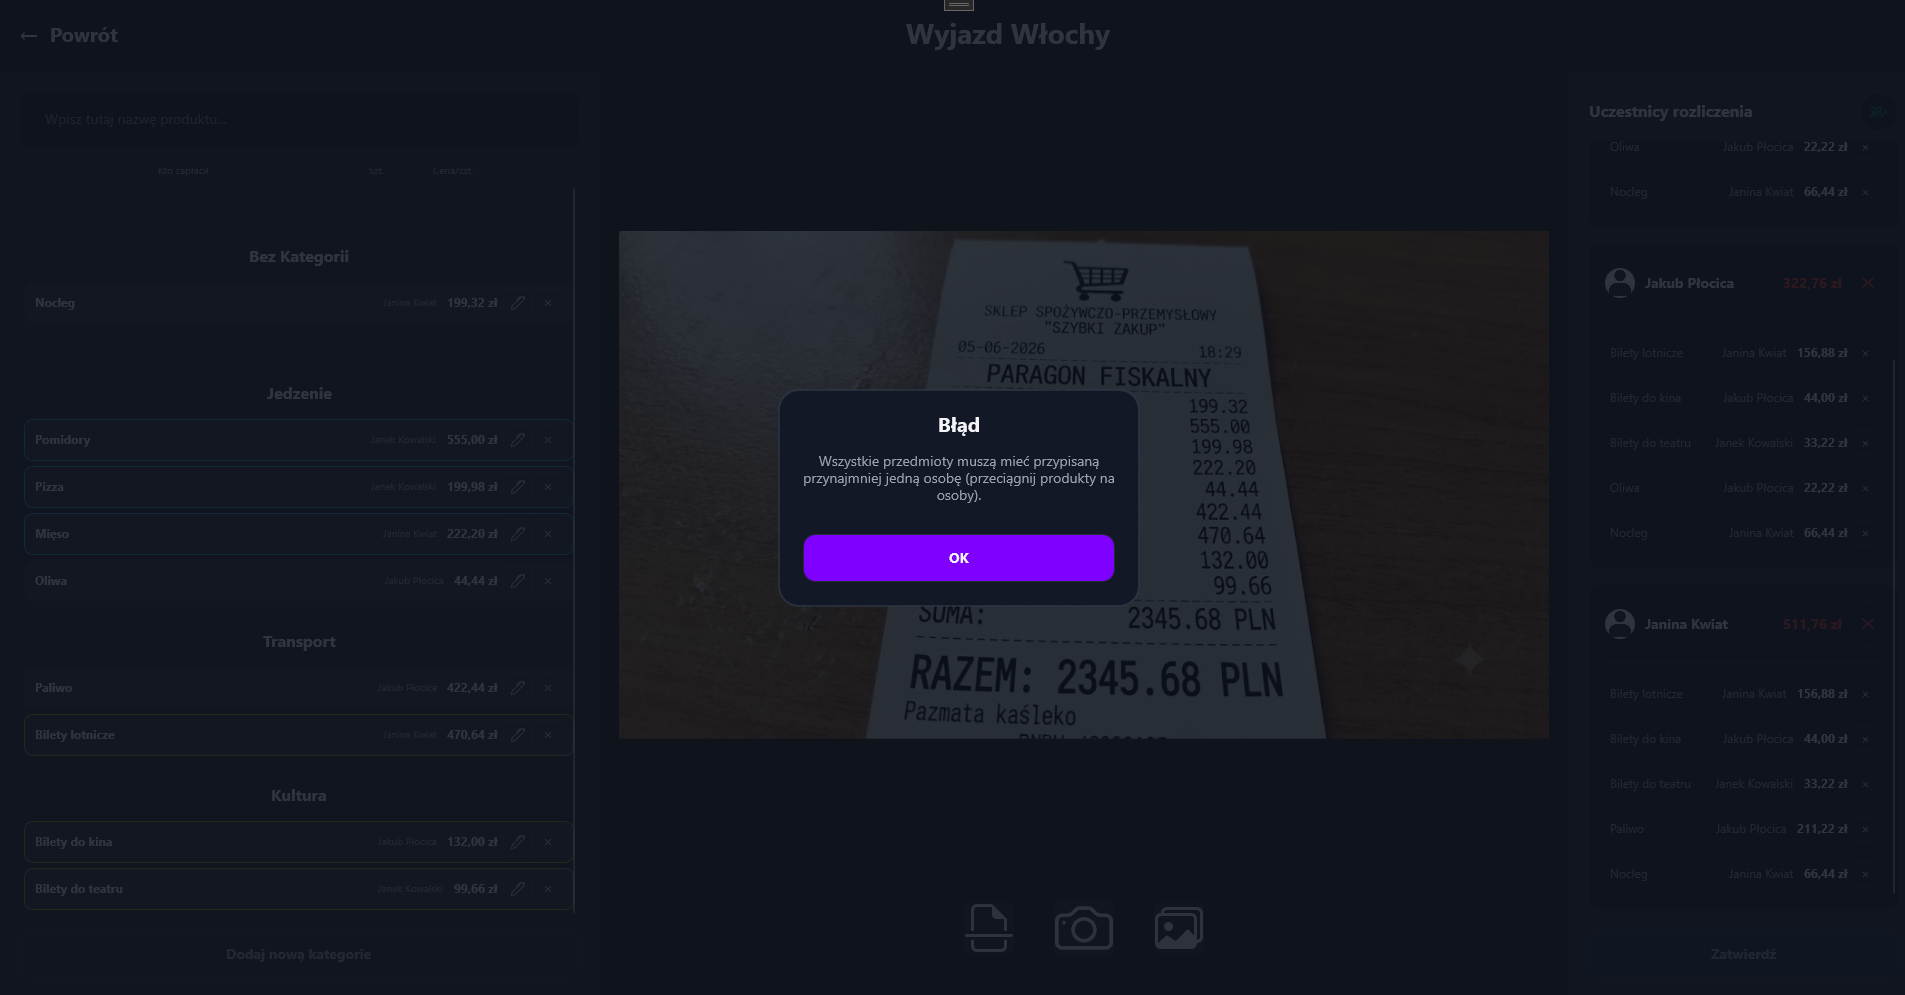
\includegraphics[width=0.95\textwidth]{img/new_expense/new_expense_blad_przy_nieprzypisaniu_wszytskiego.png}
    \vspace{0.5cm} \\
    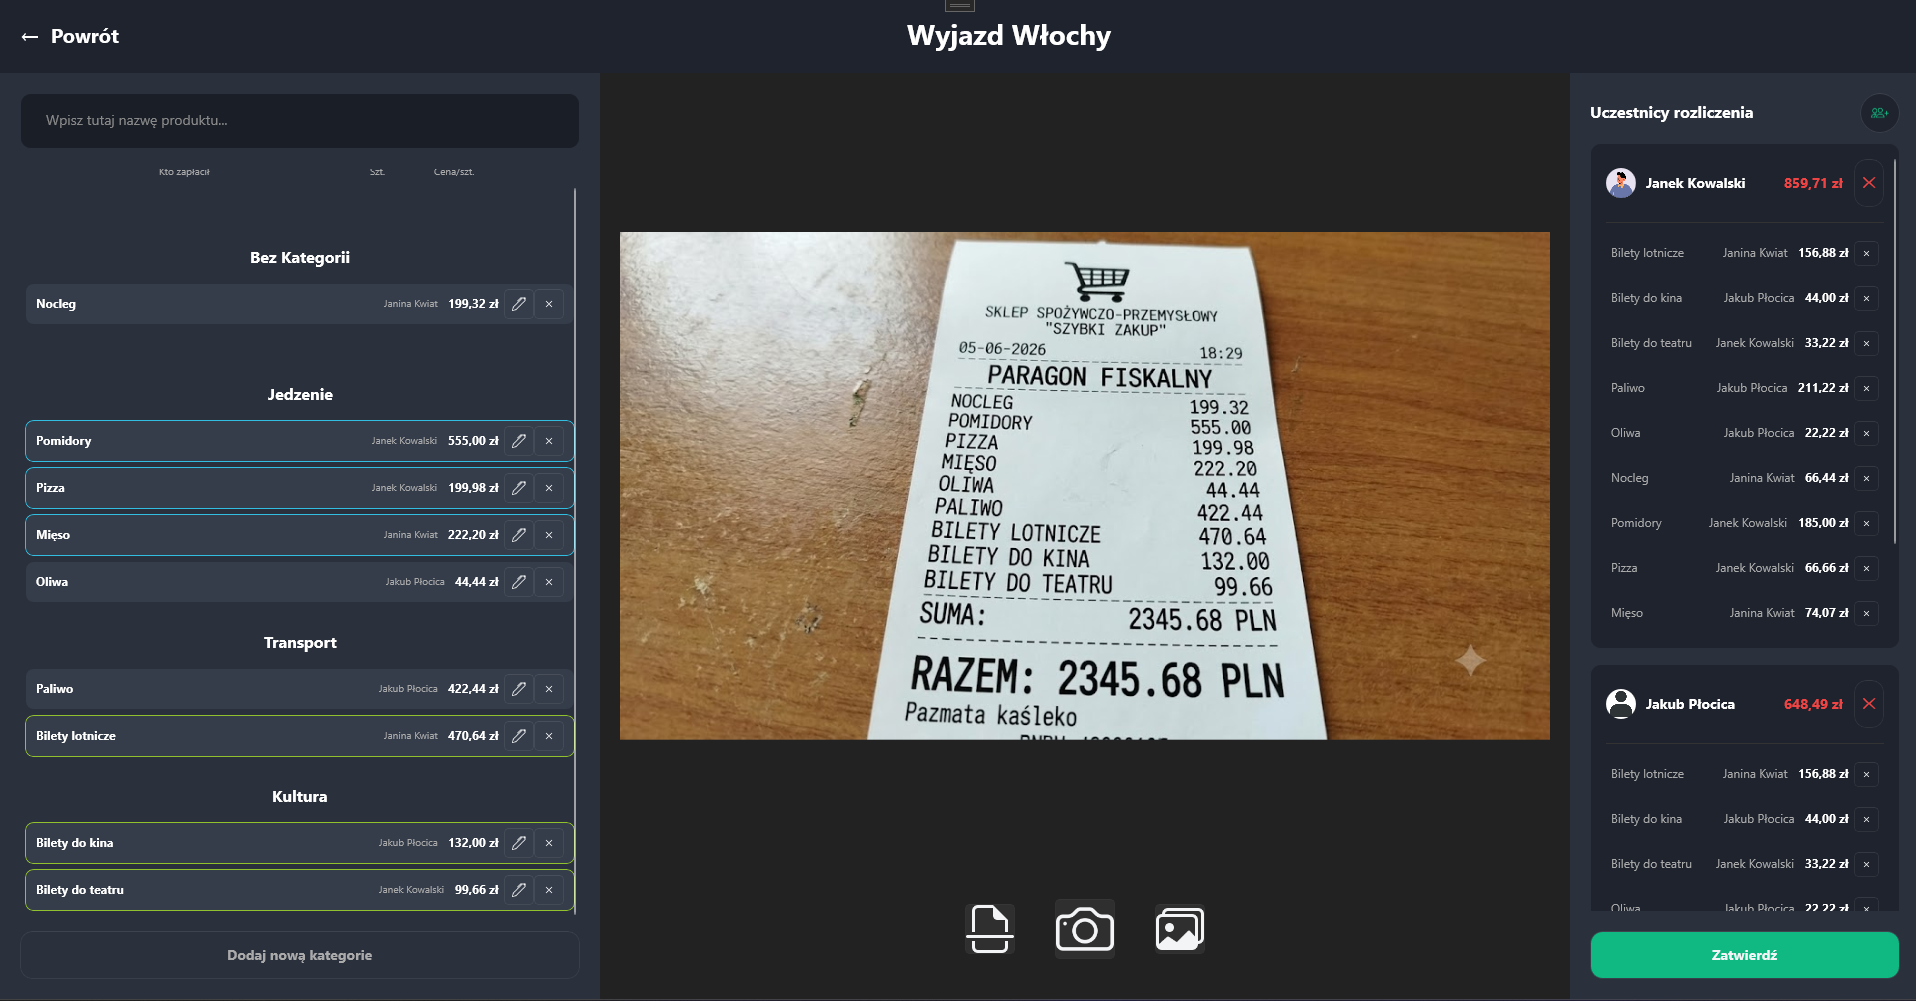
\includegraphics[width=0.95\textwidth]{img/new_expense/new_expense_ostateczny_widok.png}
    \vspace{0.5cm} \\
    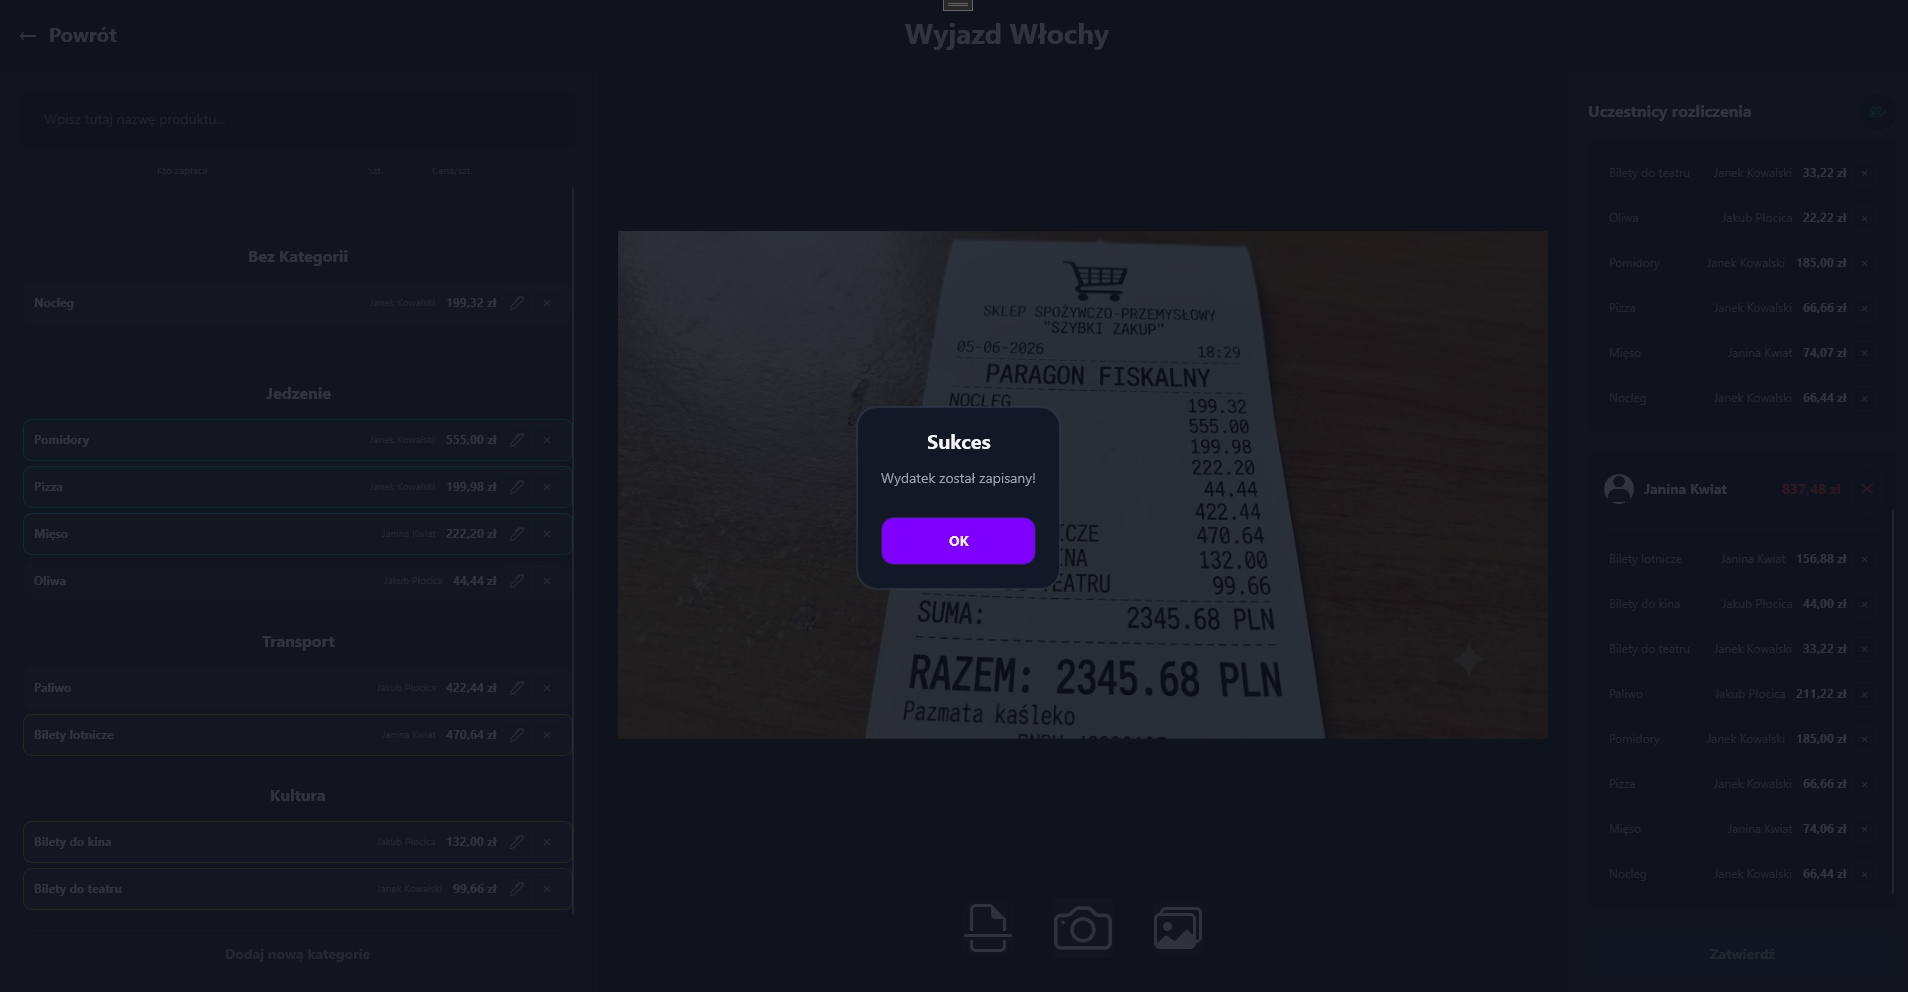
\includegraphics[width=0.95\textwidth]{img/new_expense/new_expense_success.png}
    \captionof{figure}{Rozwiązanie problemu reszty (Penny-Drop). Blokada zapisu przy ułamkowym nieprzypisaniu kwoty, finalne podsumowanie (Summary) i potwierdzenie sukcesu operacji serwerowej.}
\end{center}


\subsection{Krok 6: Inspekcja i Monitorowanie}
Zakładka przeglądu historii grupy. Użytkownicy w każdej chwili mogą cofnąć się w czasie, odnaleźć archiwalny wydatek i zajrzeć w szczegółowy Drill-Down podziału kosztów.

\begin{center}
    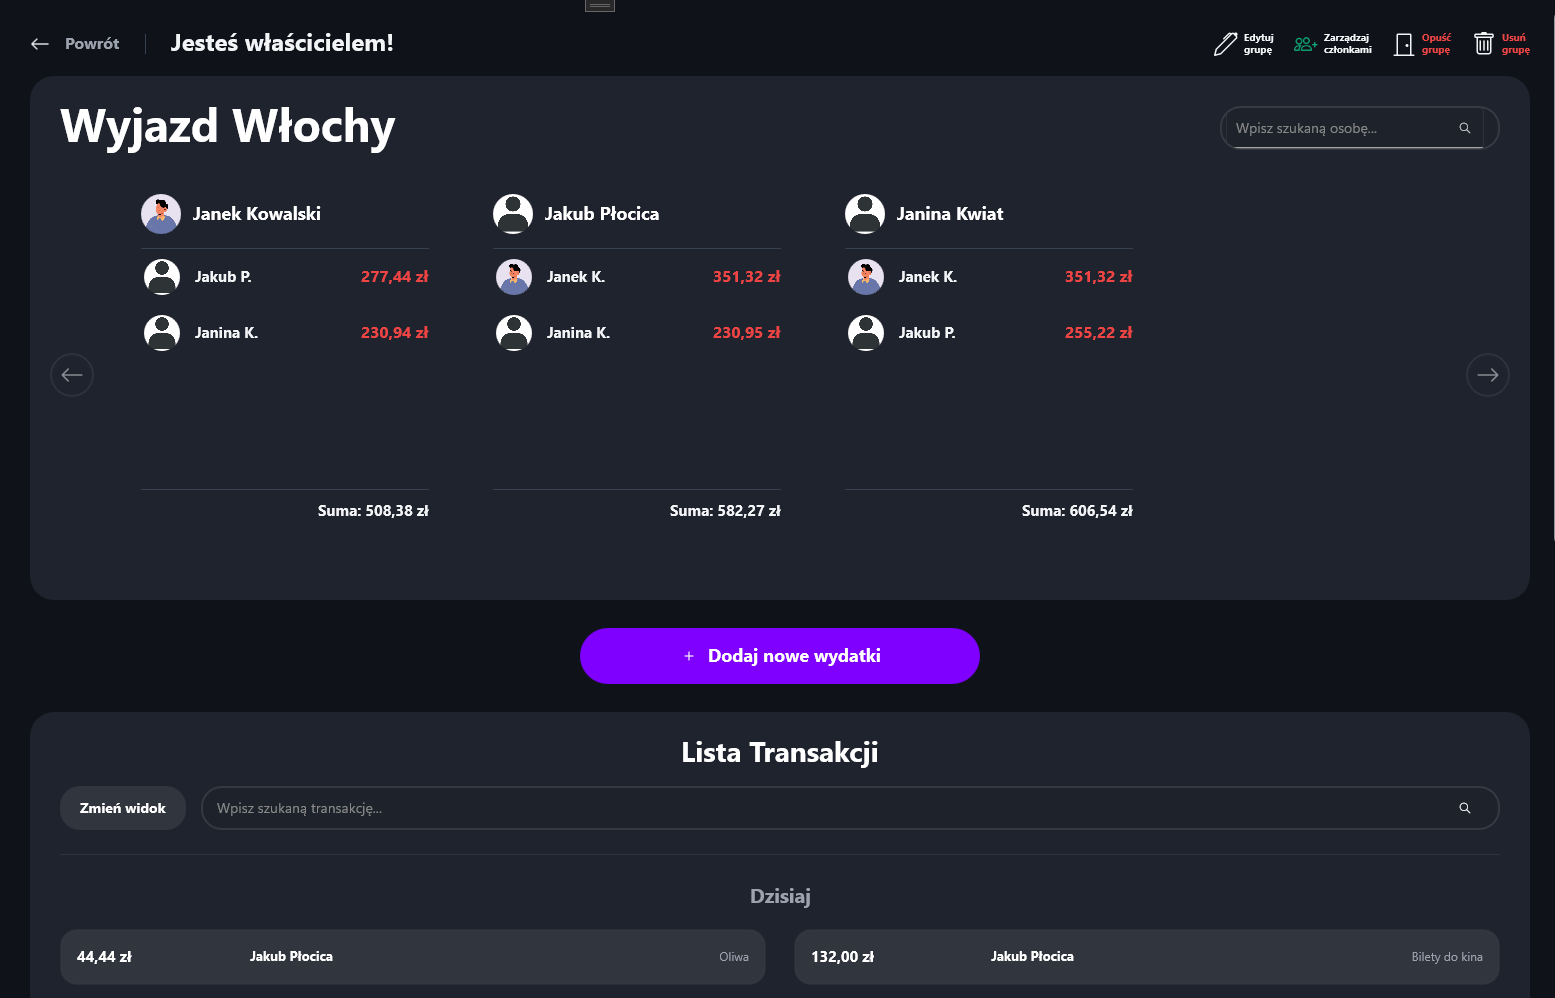
\includegraphics[width=0.95\textwidth]{img/group/group_widok_po_dodaniu_wydatków.png}
    \vspace{0.5cm} \\
    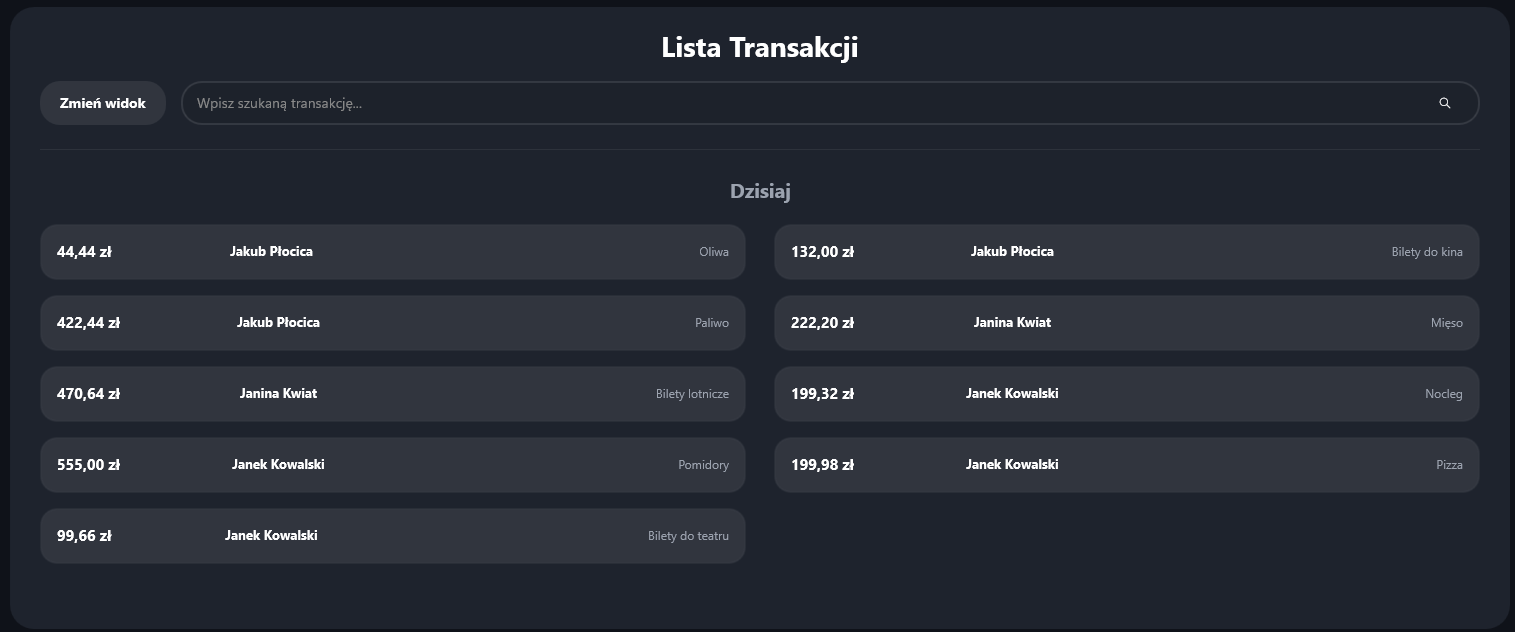
\includegraphics[width=0.95\textwidth]{img/group/group_widok_listy_transakcji.png}
    \captionof{figure}{Inspekcja finansowa wewnątrz grupy. Widoczne podsumowanie zbalansowanego salda (kto jest winien, kto ma nadpłatę) oraz historia w ujęciu chronologicznym.}
\end{center}

\begin{center}
    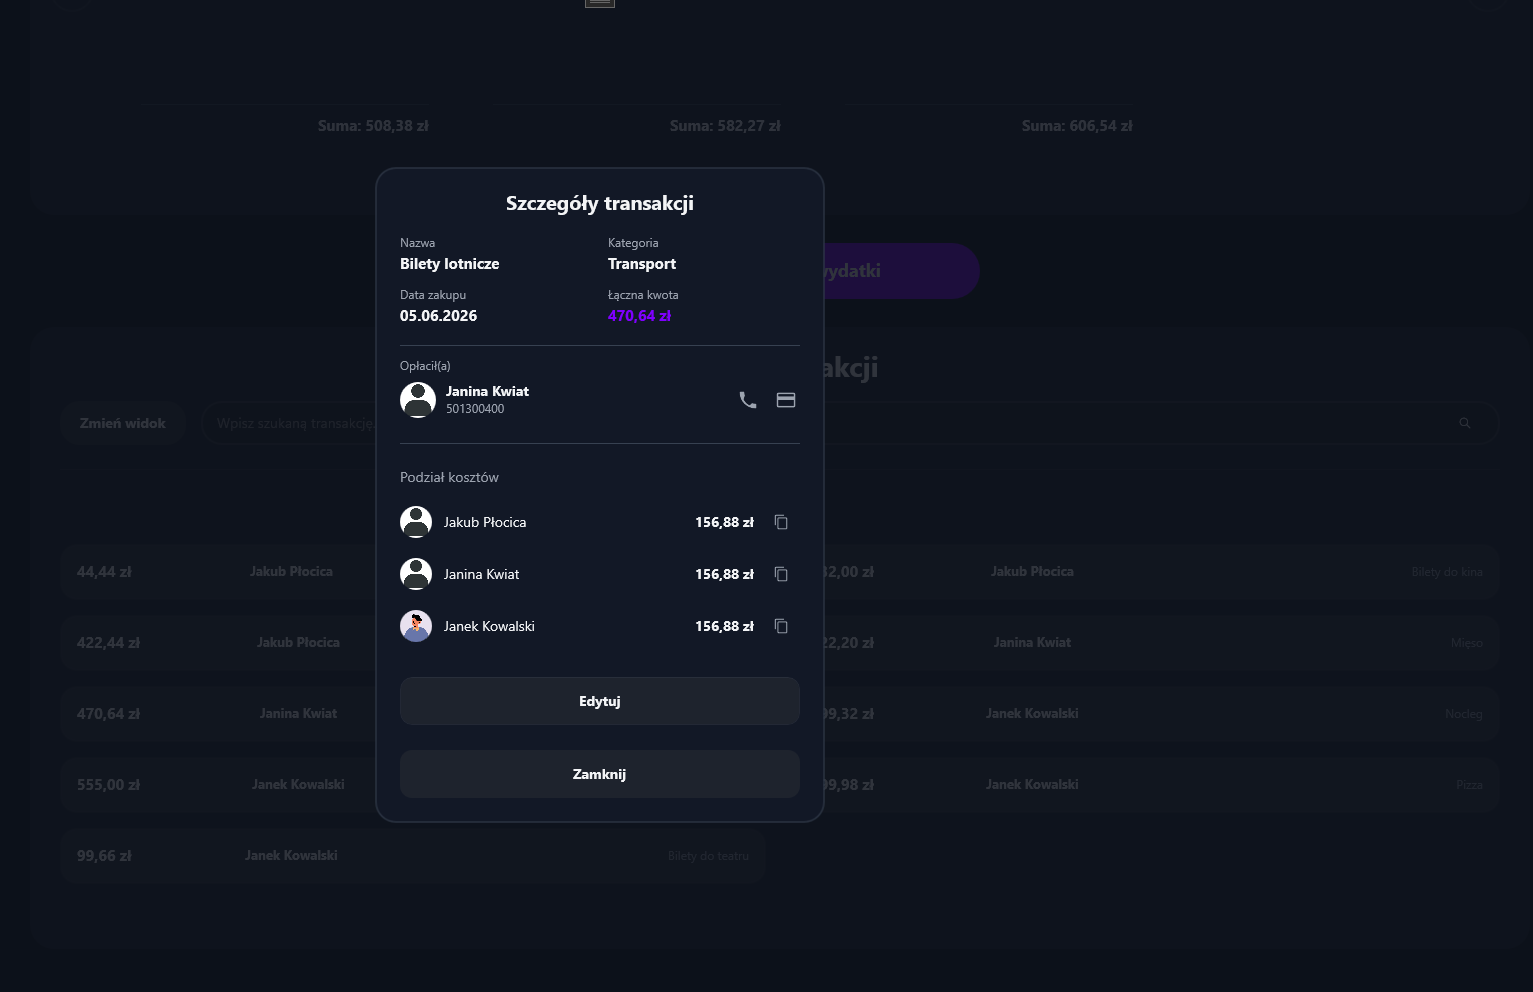
\includegraphics[width=0.95\textwidth]{img/group/group_klikniecie_w_przedmiot_na_liscie.png}
    \captionof{figure}{Szczegóły historycznego wydatku. Analiza Drill-Down umożliwiająca szybkie zweryfikowanie partycypacji kosztowej w archiwalnych rachunkach.}
\end{center}

\begin{center}
    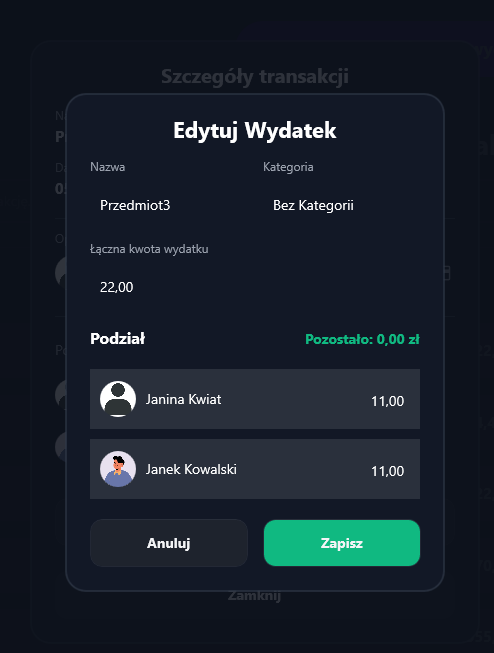
\includegraphics[width=0.45\textwidth]{img/group/group_edycja_wydatku.png}
    \hfill
    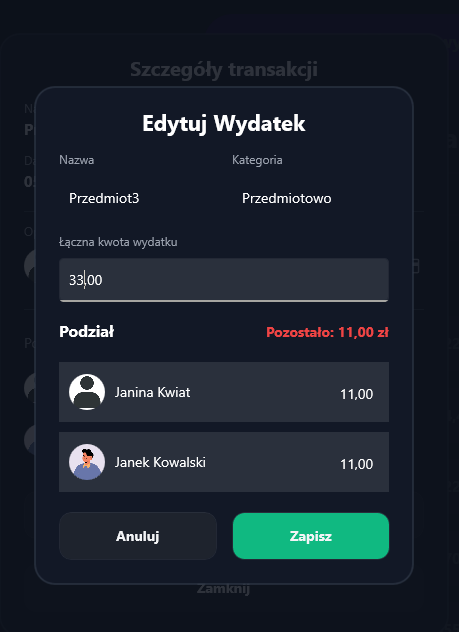
\includegraphics[width=0.45\textwidth]{img/group/group_edycja_wydatku_brak_rozlozenia.png}
    \vspace{0.5cm} \\
    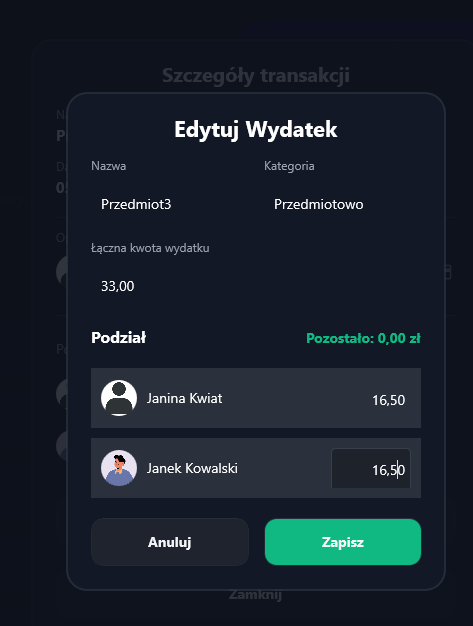
\includegraphics[width=0.45\textwidth]{img/group/group_edycja_wydatku_poprawne.png}
    \captionof{figure}{Edycja historycznego wydatku. Formularz pozwalający na modyfikację istniejących paragonów, blokada zapisu w przypadku niezbilansowania kwot oraz poprawnie rozdzielona ostateczna kwota.}
\end{center}

\begin{center}
    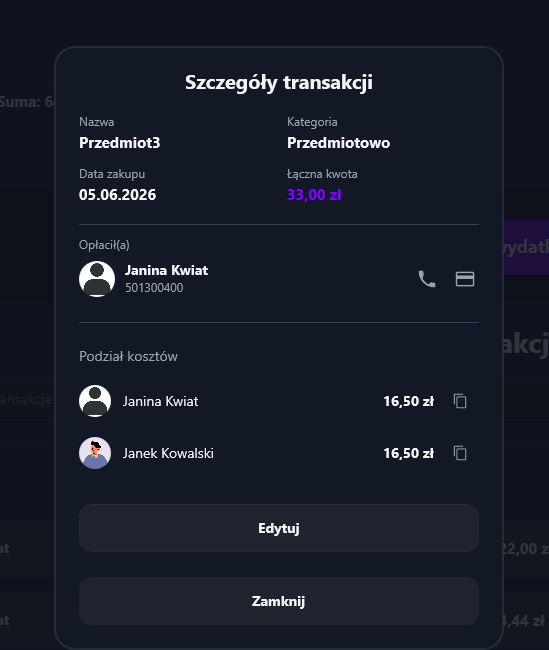
\includegraphics[width=0.45\textwidth]{img/group/group_zedytowany_wydatek.png}
    \captionof{figure}{Efekt końcowy procedury edycji. Przeliczenie i aktualizacja archiwalnego podsumowania wraz z naniesionymi nowymi kwotami zadłużeń.}
\end{center}


\subsection{Krok 7: Zamykanie Cyklu (Rozliczanie Długów)}
Ostatecznym krokiem operacji finansowej jest sprawdzenie salda i oznaczenie zwrotu pożyczki poprzez interfejs płatności. System ułatwia wysyłanie ponagleń, kompensuje długi do wartości Netto i czuwa nad uczciwością weryfikacji po stronie wierzyciela.

\begin{center}
    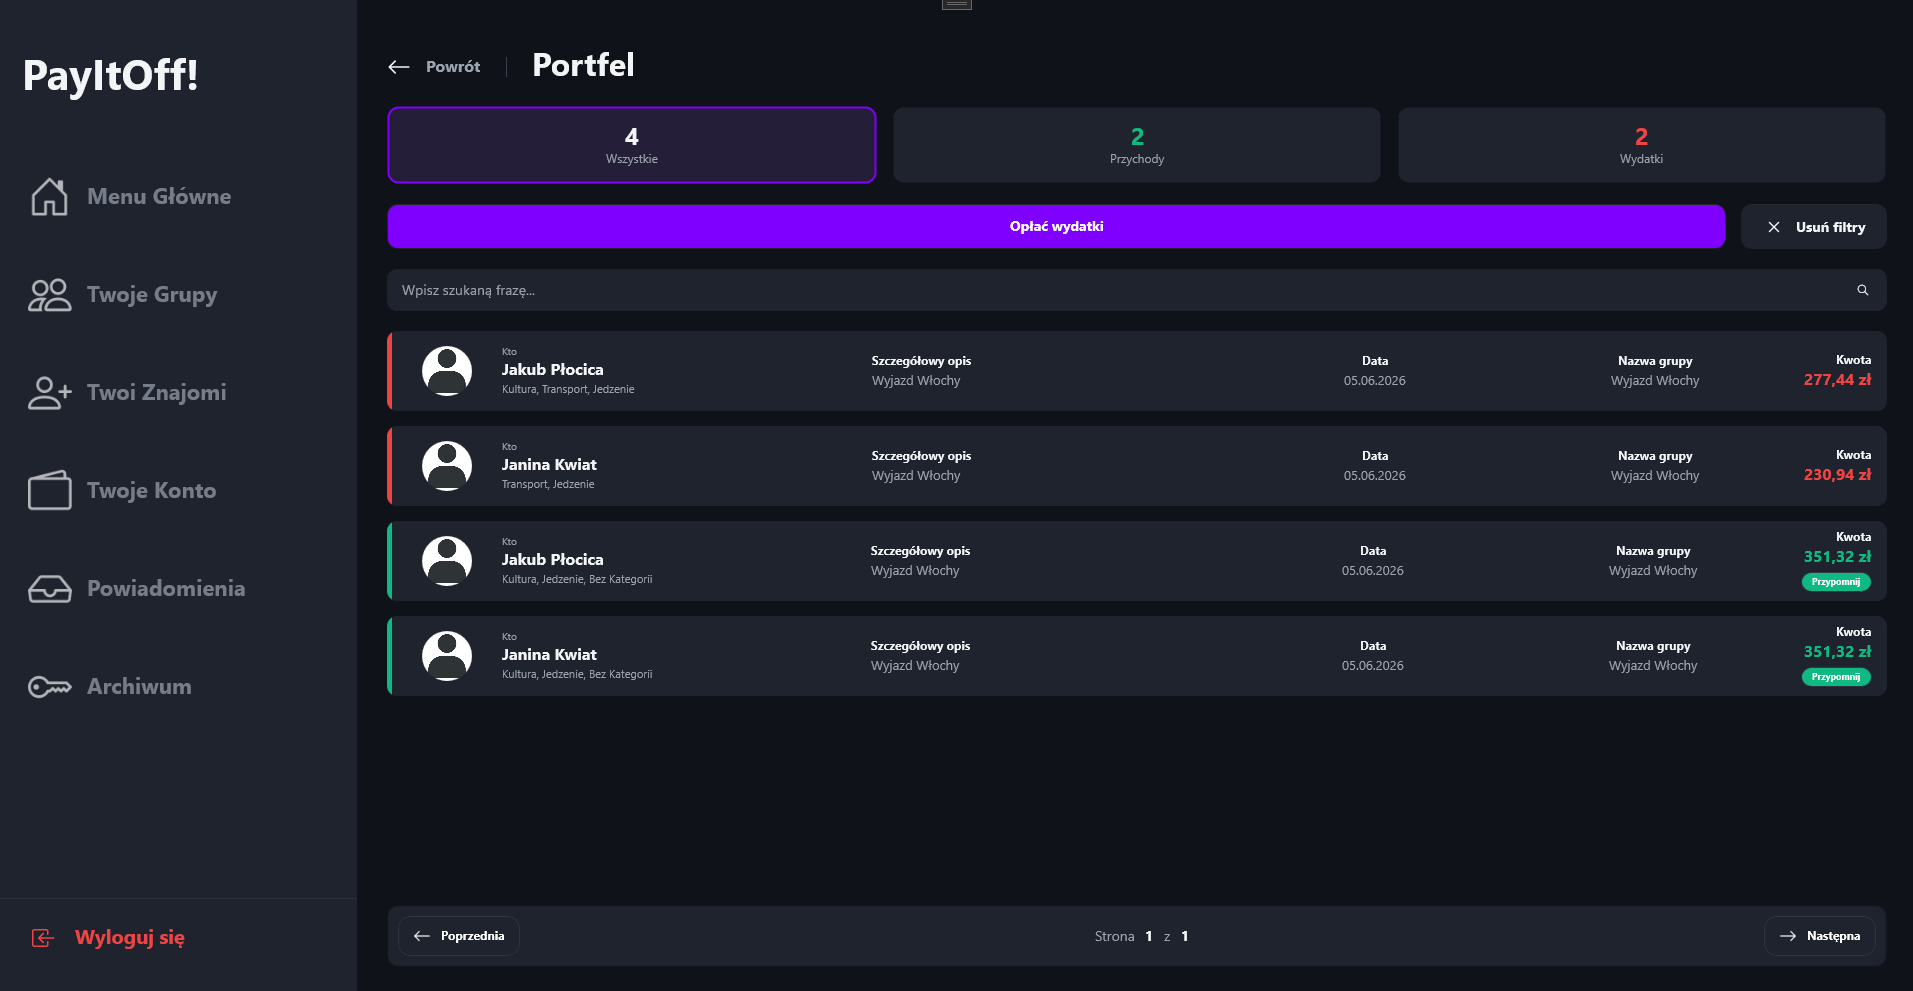
\includegraphics[width=0.95\textwidth]{img/settlement/settlement_widok_i_podzial_na_filtry.png}
    \vspace{0.5cm} \\
    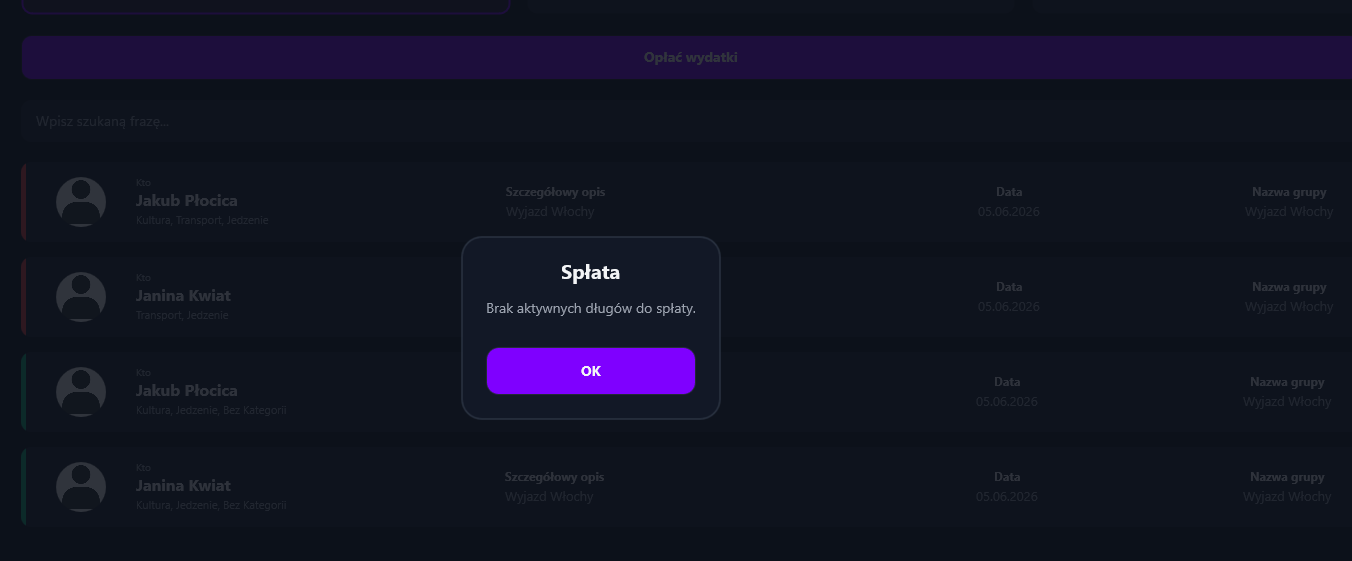
\includegraphics[width=0.95\textwidth]{img/settlement/settlement_oplacenie_dlugow_gdy_ich_nie_ma.png}
    \captionof{figure}{Moduł \textbf{Settlement}. Wszechstronny panel rozliczeniowy wyposażony w potężne filtry wektorów długu oraz miła dla oka grafika "Czystej Karty" przy wyzerowanych zobowiązaniach.}
\end{center}

\begin{center}
    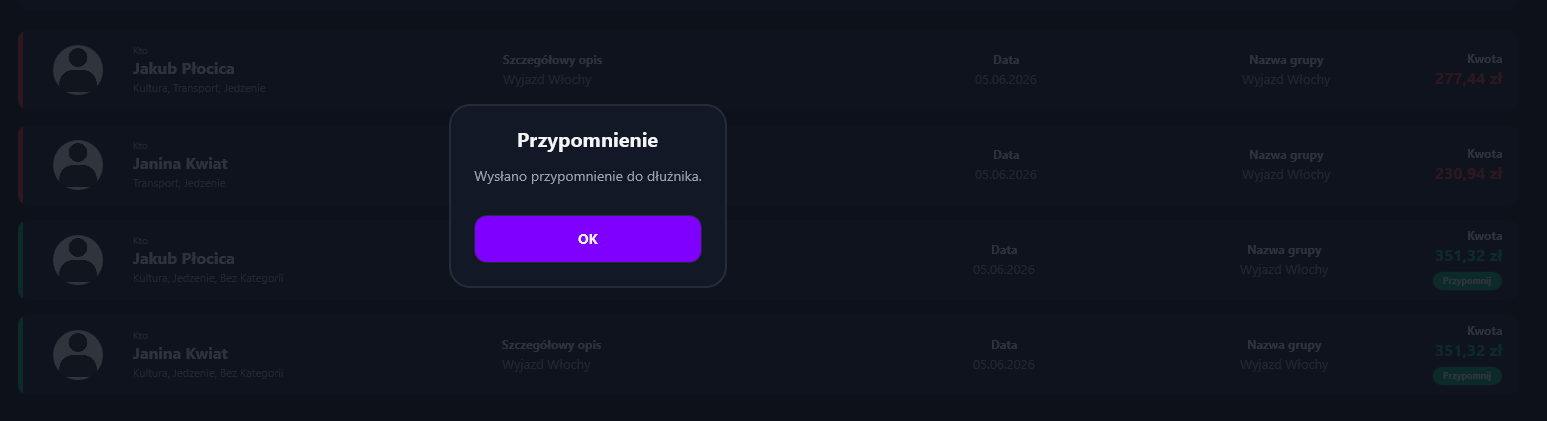
\includegraphics[width=0.95\textwidth]{img/settlement/settlement_przypomnienie.png}
    \vspace{0.5cm} \\
    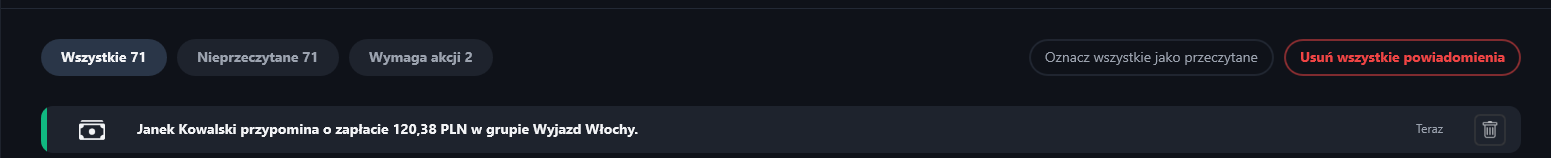
\includegraphics[width=0.95\textwidth]{img/settlement/settlement_powoadomienie_osoby_do_ktorej_poszlo_przypomnienie.png}
    \vspace{0.5cm} \\
    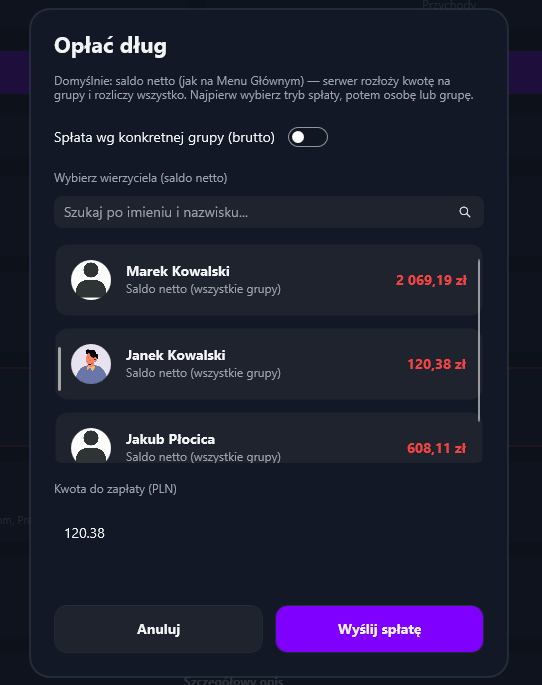
\includegraphics[width=0.45\textwidth]{img/settlement/settlement_oplacenie_netto.png}
    \captionof{figure}{Narzędzia windykacyjne. Wysłanie przypomnienia ("Nudge") do znajomego, powiadomienie Push, oraz wywołanie inteligentnego algorytmu spłaty netto minimalizującego przepływy kapitału.}
\end{center}

\begin{center}
    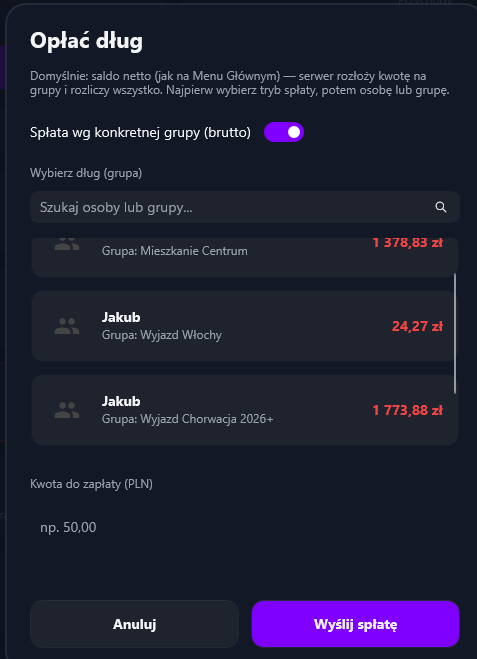
\includegraphics[width=0.45\textwidth]{img/settlement/settlement_oplacenie_brutto.png}
    \hfill
    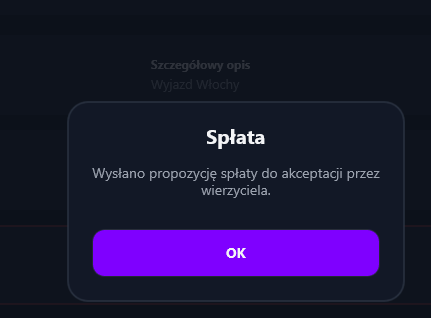
\includegraphics[width=0.45\textwidth]{img/settlement/settlement_success_wyslania_oplacenie.png}
    \vspace{0.5cm} \\
    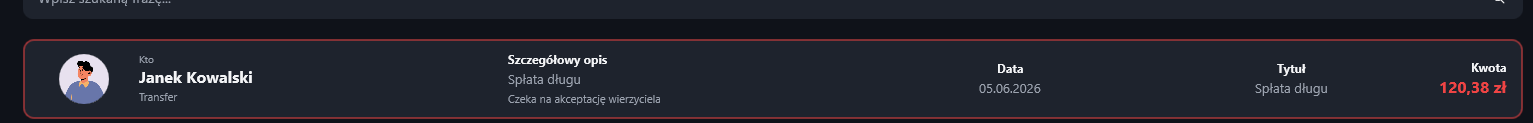
\includegraphics[width=0.95\textwidth]{img/settlement/settlement_wyslana_splata_do_akceptacji.png}
    \captionof{figure}{Inicjacja przelewu kompensującego. Przebieg rozliczenia klasycznego (brutto), ekran potwierdzenia systemowego i zmiana statusu należności na oczekującą (Pending).}
\end{center}

\begin{center}
    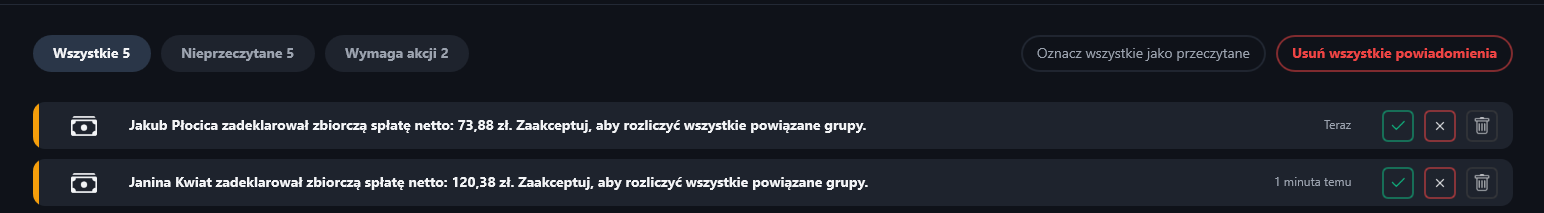
\includegraphics[width=0.95\textwidth]{img/settlement/settlement_powiadomienia_wierzyciela_o_splatach.png}
    \vspace{0.5cm} \\
    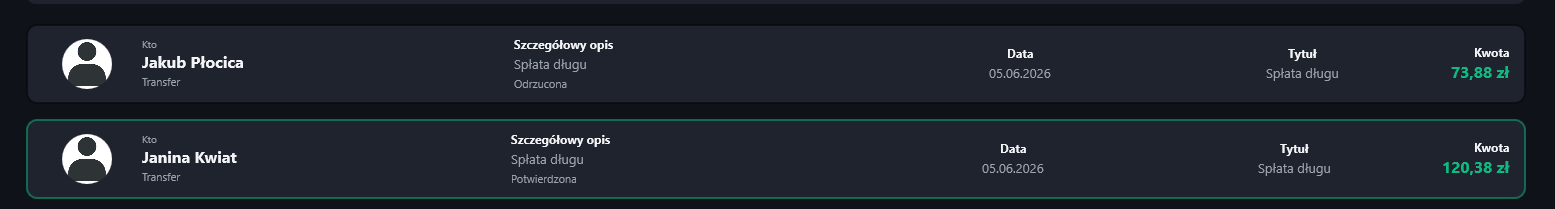
\includegraphics[width=0.95\textwidth]{img/settlement/settlement_zmiana_widokow_splat.png}
    \captionof{figure}{Perspektywa Wierzyciela. Otrzymanie powiadomienia wymuszającego podjęcie akcji oraz odfiltrowanie żądań wymagających zweryfikowania zaksięgowania na koncie w banku.}
\end{center}

\begin{center}
    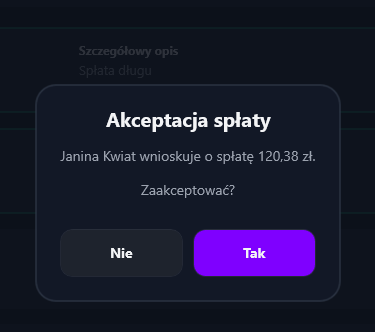
\includegraphics[width=0.45\textwidth]{img/settlement/settlement_potwierdzenie_splaty.png}
    \hfill
    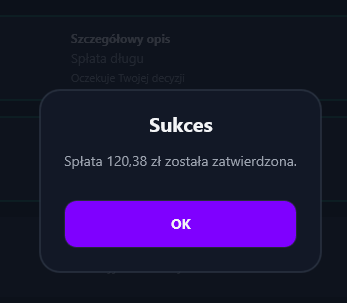
\includegraphics[width=0.45\textwidth]{img/settlement/settlement_potwierdzenie_splaty_success.png}
    \vspace{0.5cm} \\
    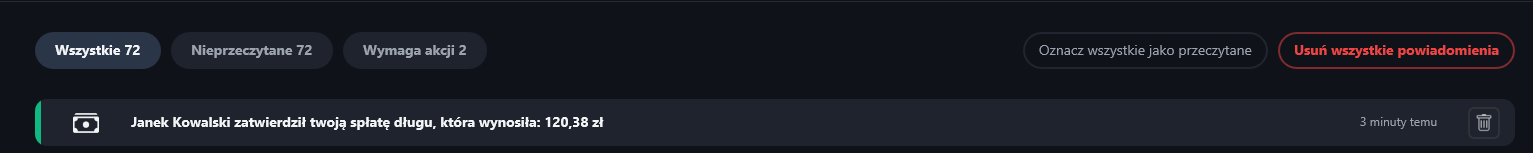
\includegraphics[width=0.95\textwidth]{img/settlement/settlement_powiadomienie_po_ackeptacji.png}
    \captionof{figure}{Zamknięcie pomyślnego cyklu życia długu. Wierzyciel zatwierdza odbiór płatności, aplikacja redukuje graf zadłużenia i posyła potwierdzenie zwrotne (notyfikację) do rzetelnego dłużnika.}
\end{center}

\begin{center}
    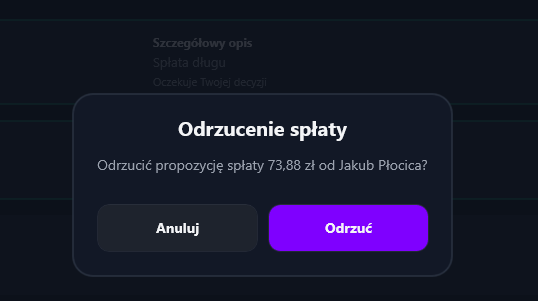
\includegraphics[width=0.45\textwidth]{img/settlement/settlement_odrzucenie_splaty.png}
    \hfill
    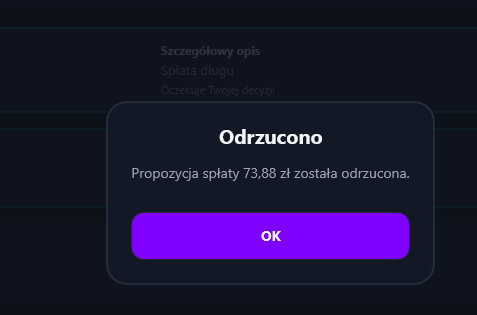
\includegraphics[width=0.45\textwidth]{img/settlement/settlement_odrzucenie_splaty_success.png}
    \vspace{0.5cm} \\
    
\includegraphics[width=0.95\textwidth]{img/settlement/settlement_powiadomienie_po_odrzuceniu.png}
    \captionof{figure}{Odrzucenie fałszywego zwrotu środków (ochrona Fake-Pay). Odrzucenie deklaracji, odtworzenie wyjściowego długu i zasygnalizowanie problemu nierzetelnemu płatnikowi komunikatem błędu.}
\end{center}

\subsection{Krok 8: Centrum Powiadomień}
Aplikacja wyposażona jest w globalne centrum powiadomień, które agreguje zdarzenia takie jak zaproszenia, przypomnienia o długach czy modyfikacje wydatków. System wspiera masowe oznaczanie powiadomień jako przeczytane oraz ich grupowe usuwanie.

\begin{center}
    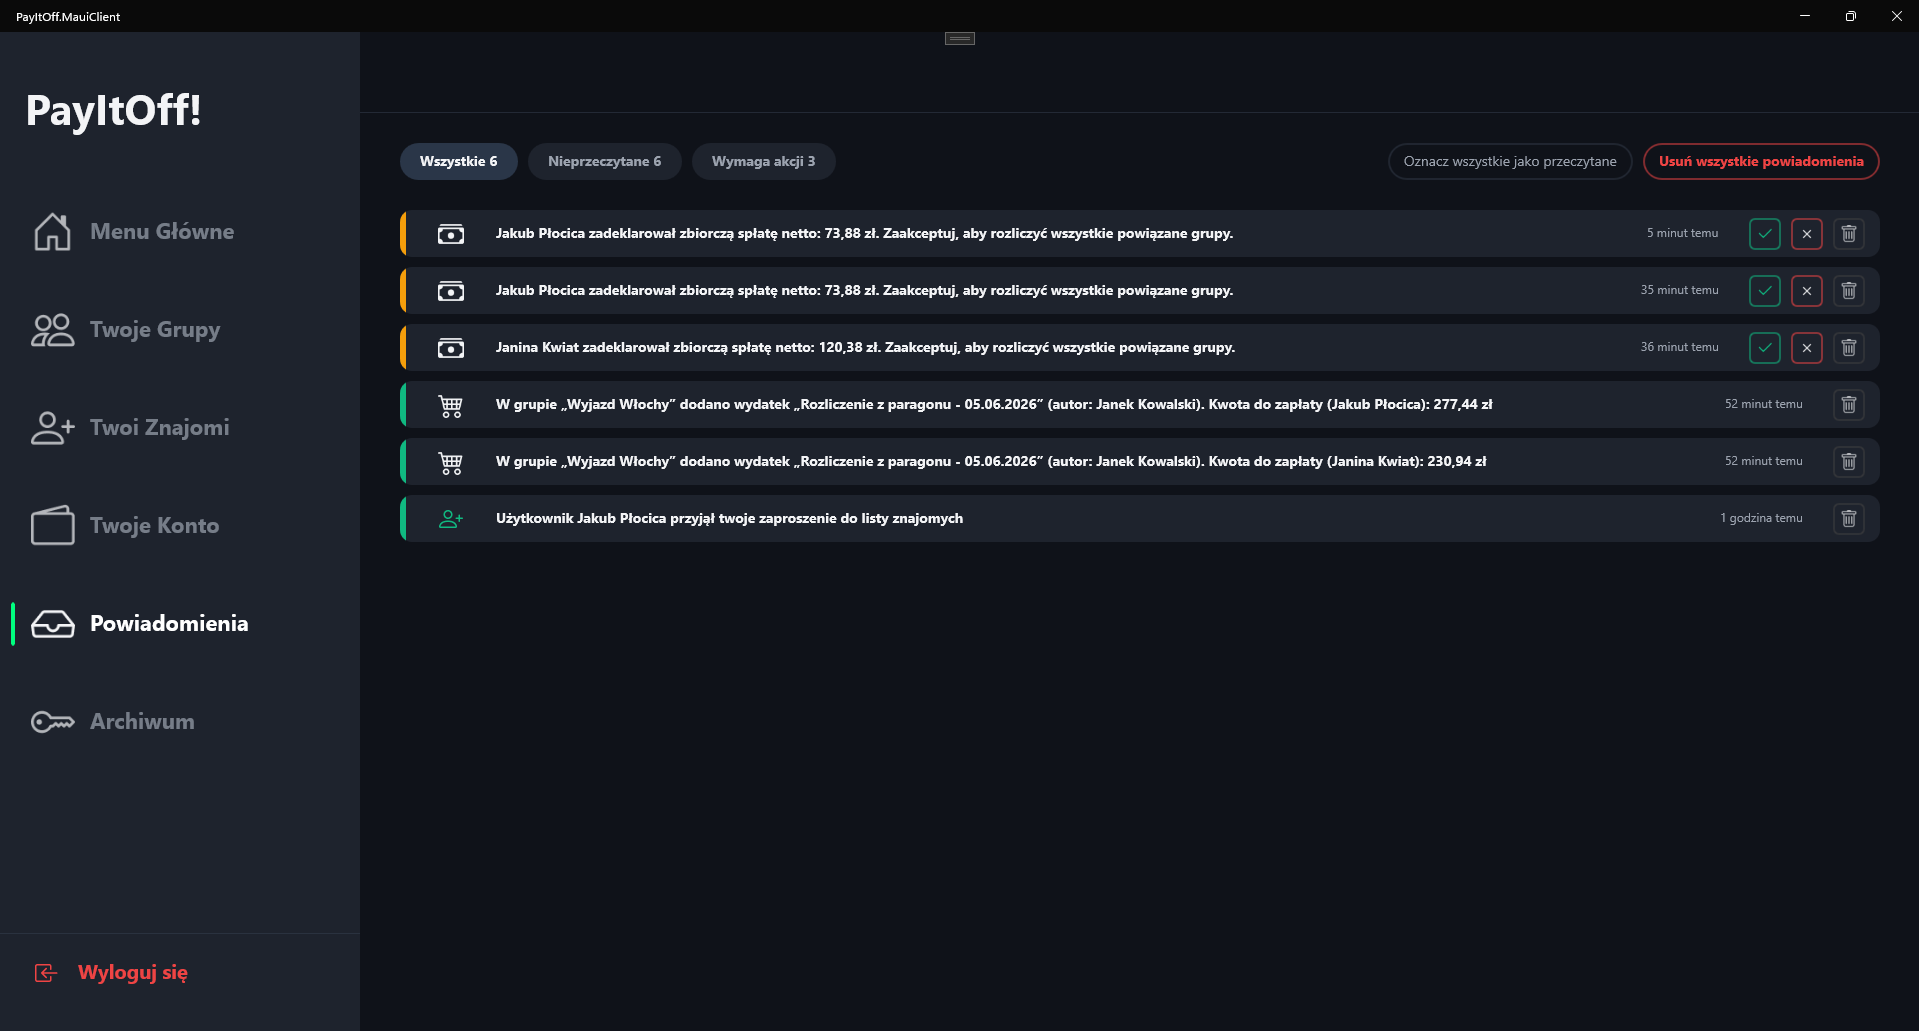
\includegraphics[width=0.95\textwidth]{img/powiadomienia/powiadomienia_widok_glowny.png}
    \vspace{0.5cm} \\
    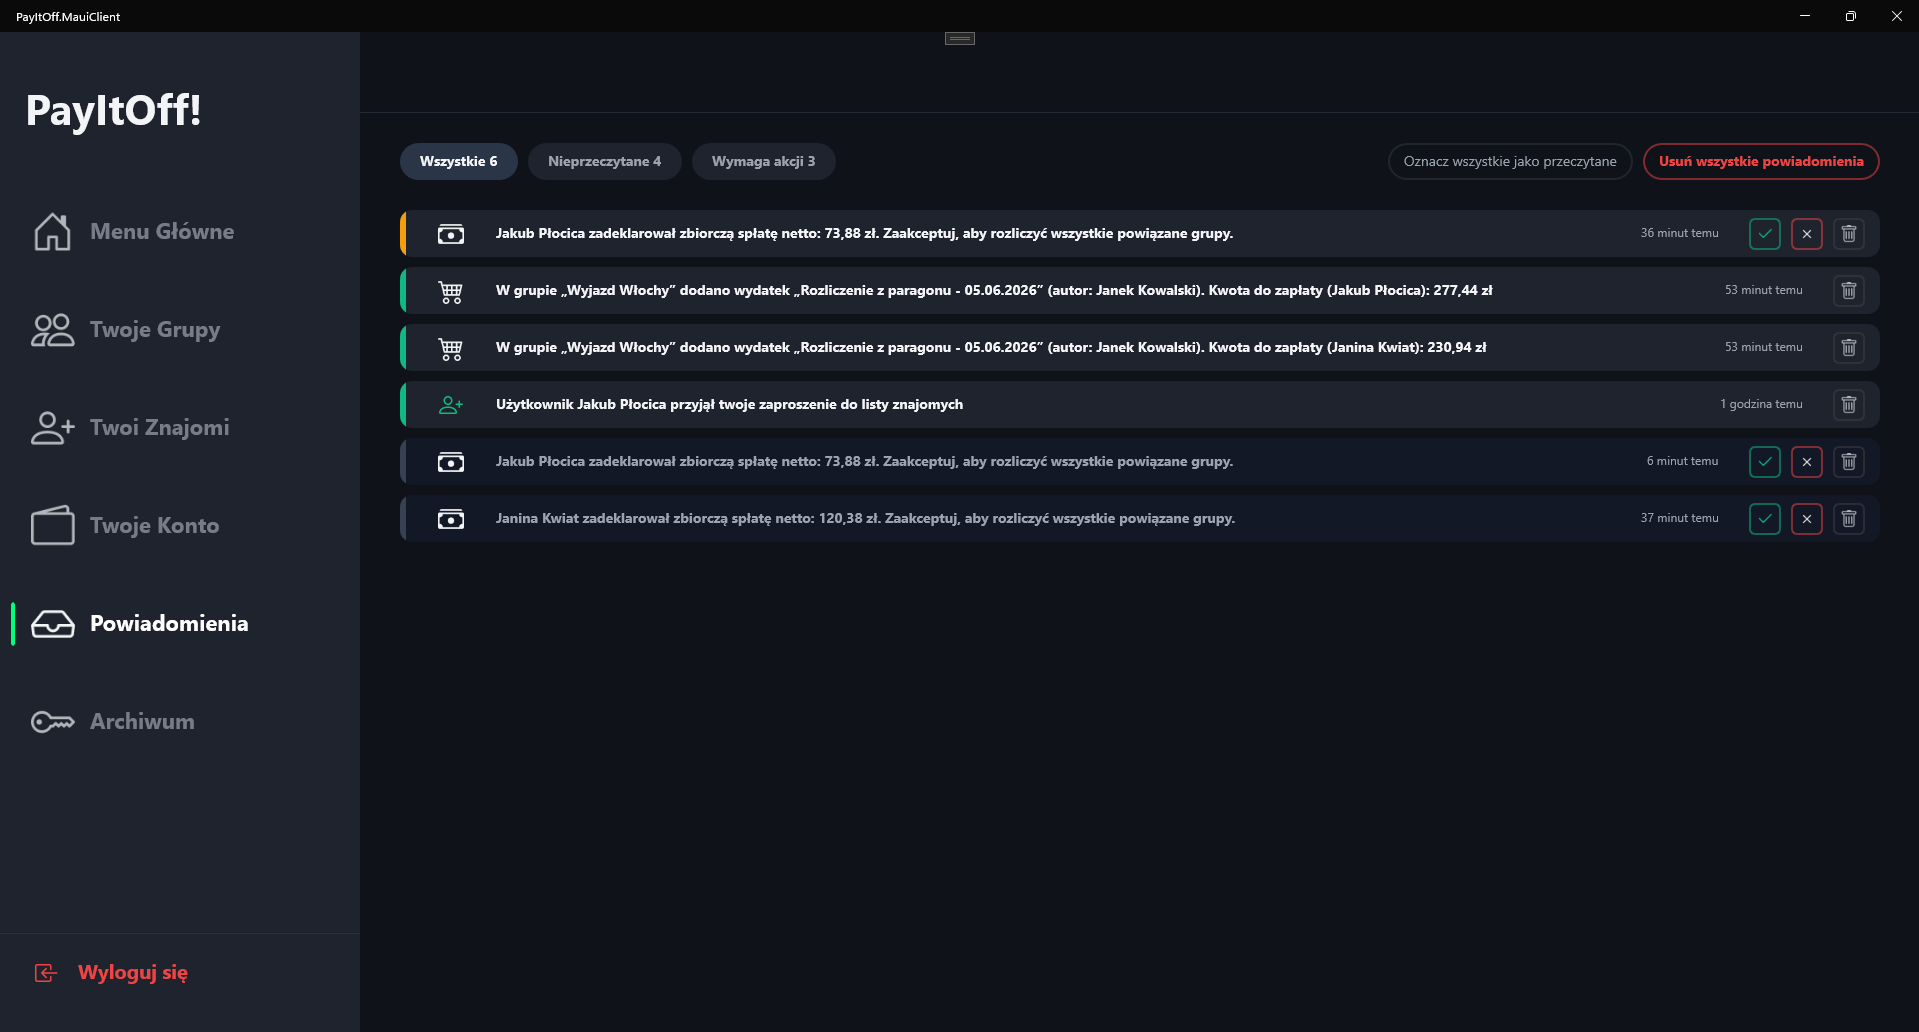
\includegraphics[width=0.95\textwidth]{img/powiadomienia/powiadomienia_widok_po_kliknieicu_w_powiadomienie.png}
    \vspace{0.5cm} \\
    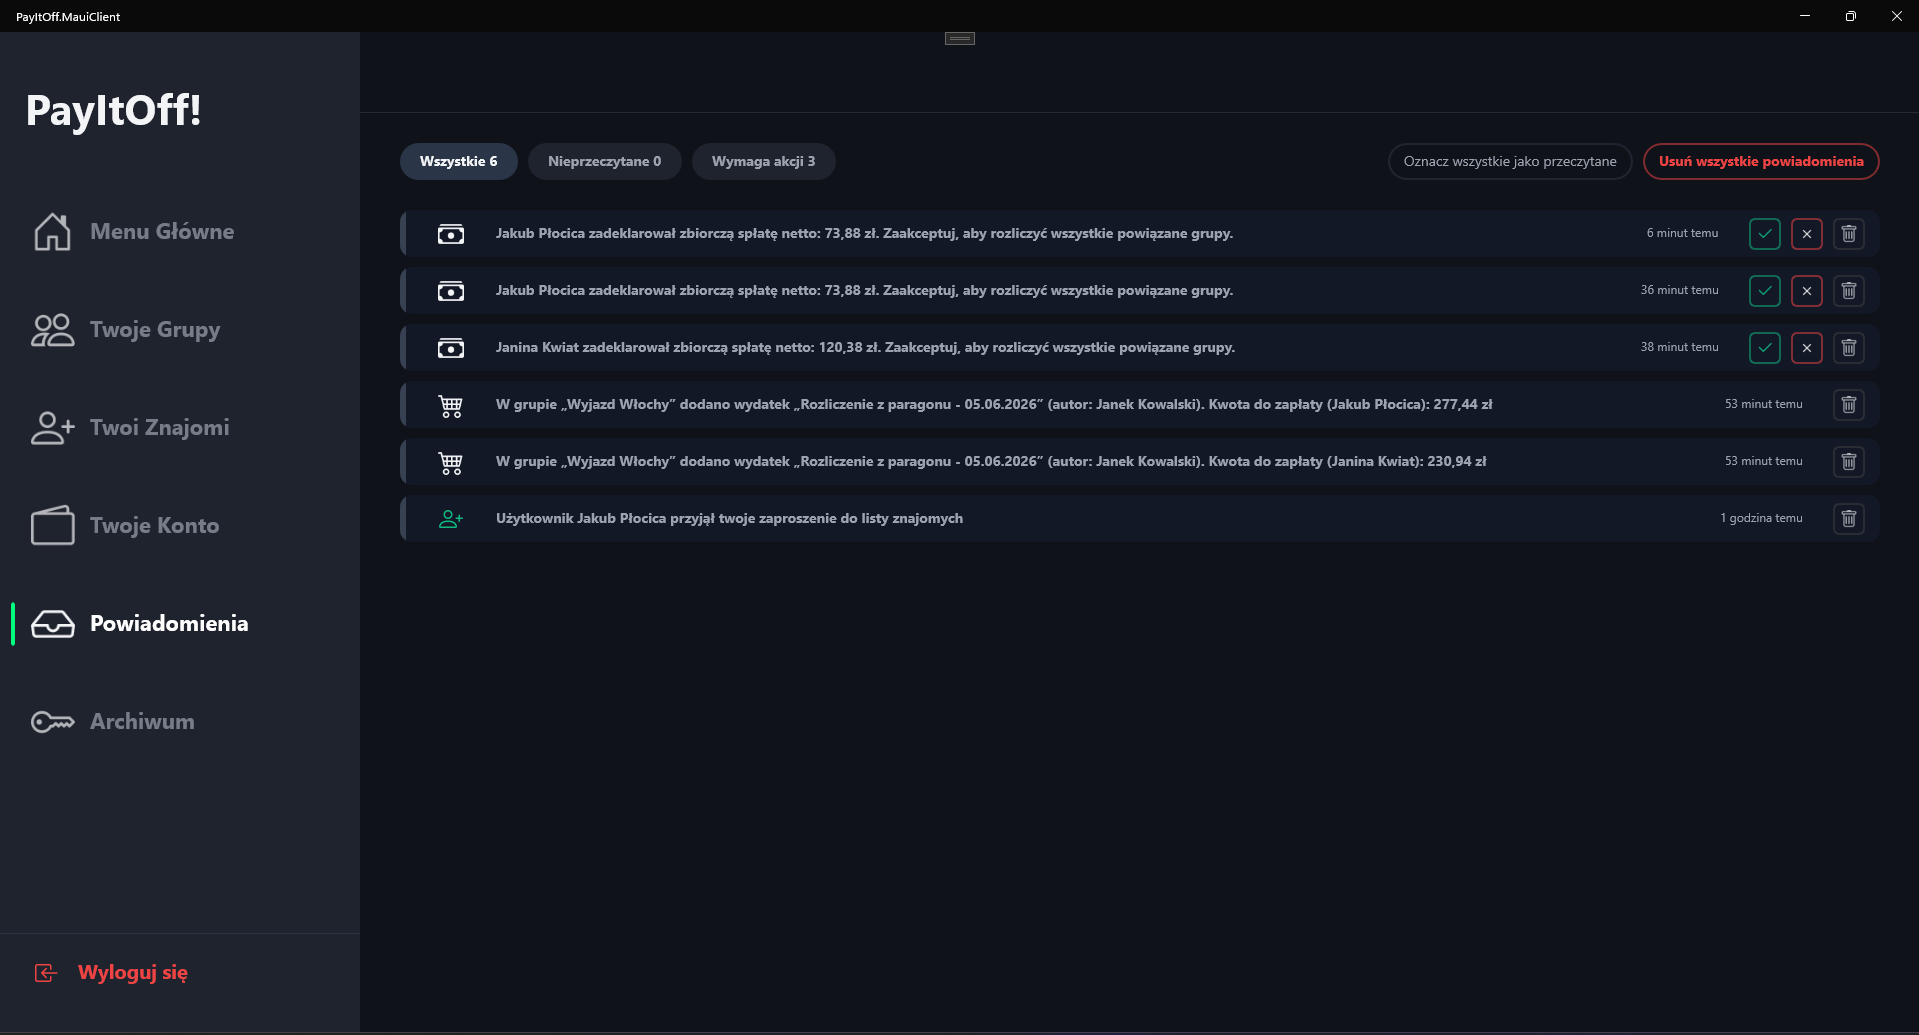
\includegraphics[width=0.95\textwidth]{img/powiadomienia/powiadomienia_oznacz_wszytskie.png}
    \captionof{figure}{Główny widok notyfikacji. Obsługa stanów przeczytanych/nieprzeczytanych oraz szybkie oznaczanie wszystkich powiadomień.}
\end{center}

\begin{center}
    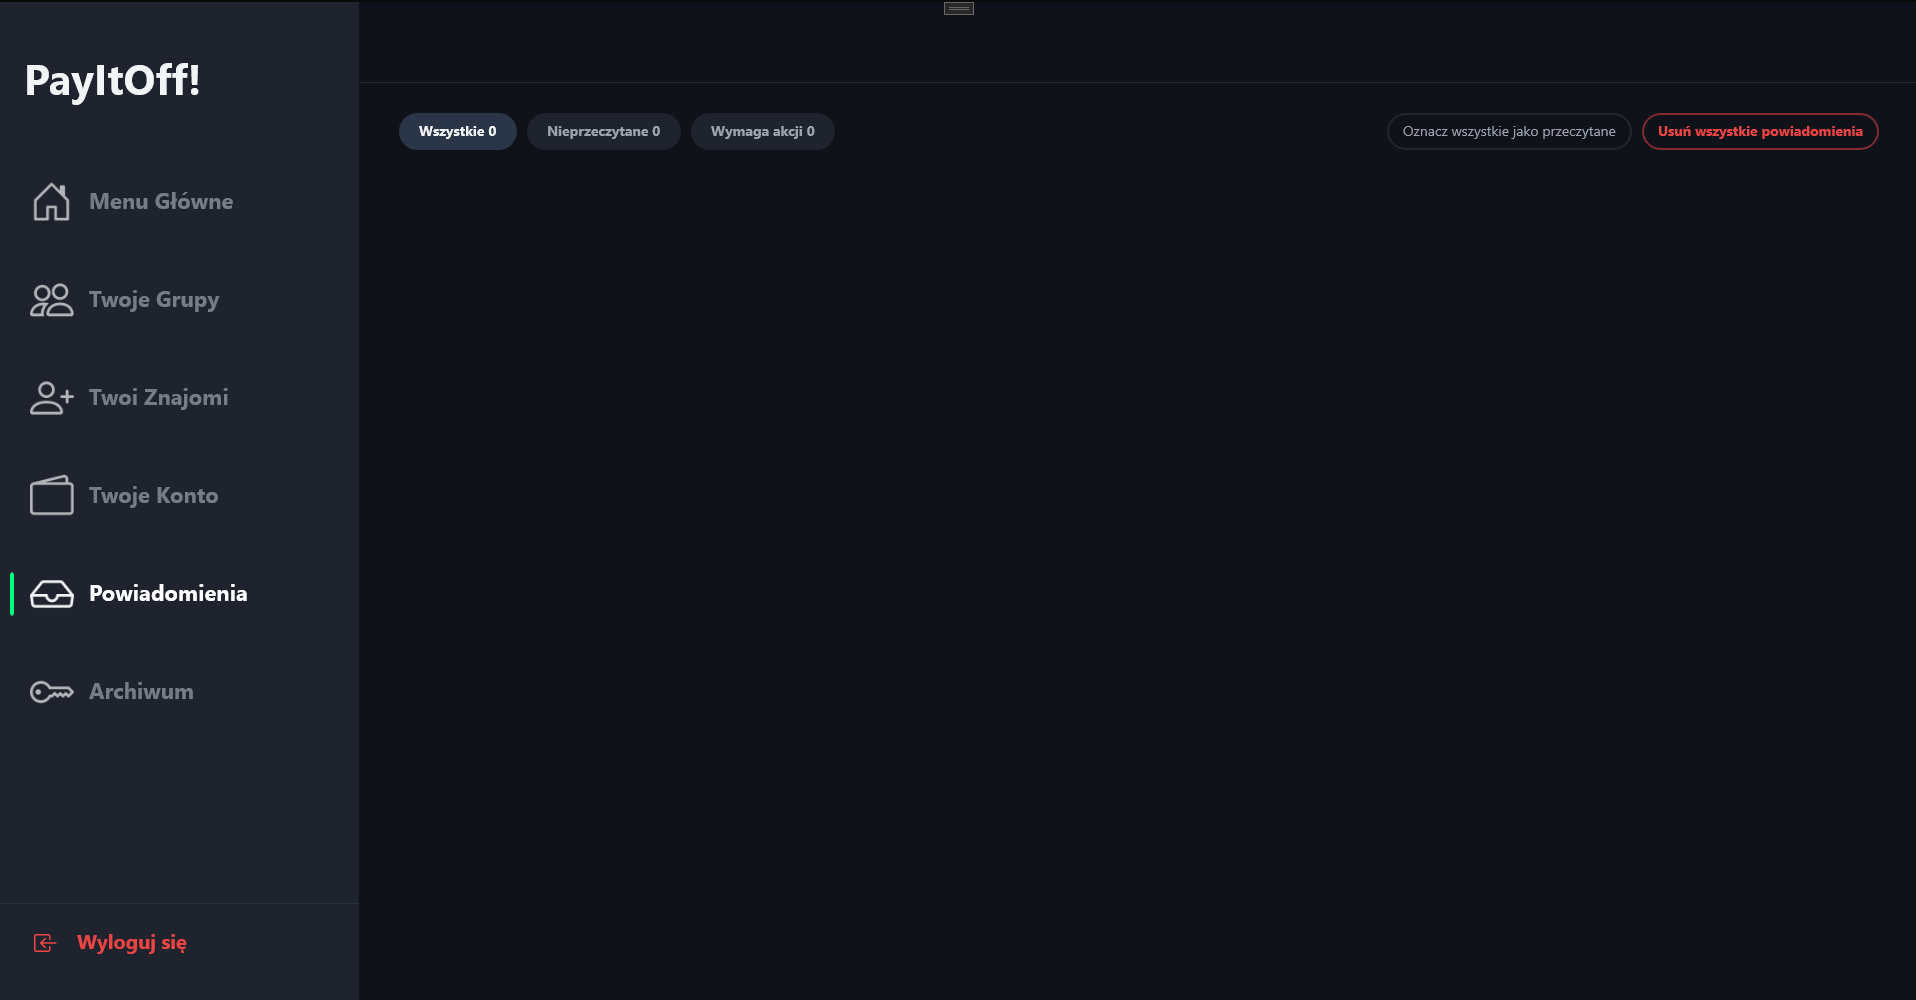
\includegraphics[width=0.95\textwidth]{img/powiadomienia/powiadomienia_usun_wszytskie.png}
    \vspace{0.5cm} \\
    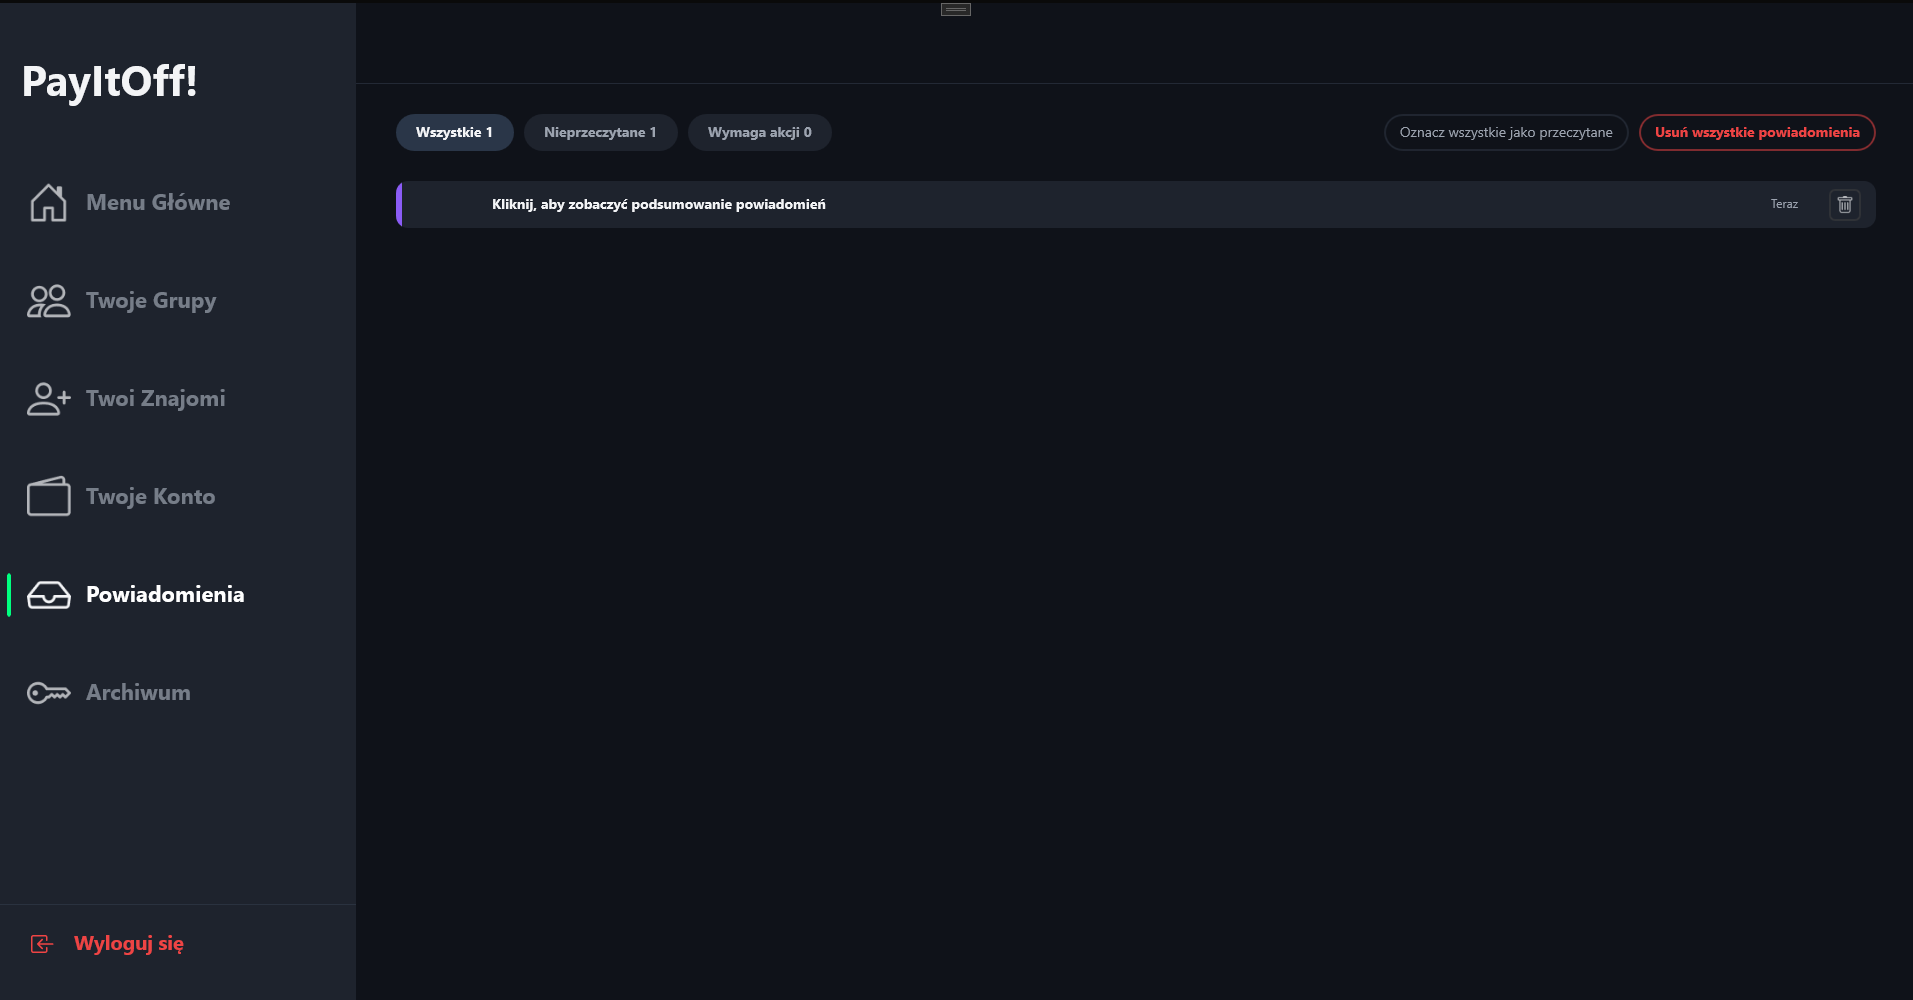
\includegraphics[width=0.95\textwidth]{img/powiadomienia/powiadomienia_zbiorcze_eytkieta.png}
    \vspace{0.5cm} \\
    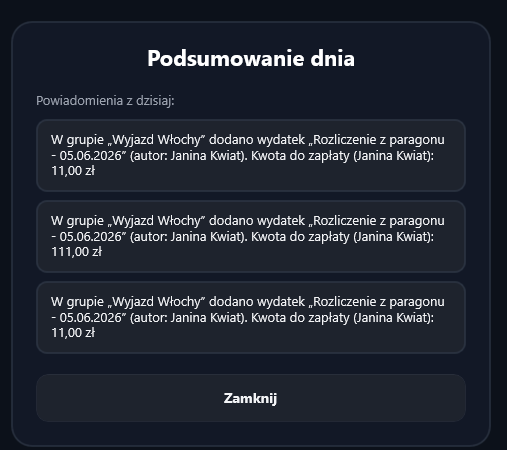
\includegraphics[width=0.45\textwidth]{img/powiadomienia/powiadomienia_zbiorcze_popup.png}
    \captionof{figure}{Funkcja czyszczenia skrzynki oraz obsługa inteligentnych powiadomień zbiorczych generowanych codziennie przez proces w tle (Hangfire).}
\end{center}

\subsection{Krok 9: Archiwizacja i Retencja Danych}
Ostatni etap cyklu życia to bezpieczne zamykanie nieaktywnych grup (Soft-Delete) lub całkowite usunięcie danych. Zgodnie z wdrożonym wzorcem miękkiego usuwania na kolumnie \texttt{DeletedAt}, pozbycie się grup czy historycznych wydatków chroni relacyjne drzewo zależności w bazie. Zarchiwizowane pozycje trafiają do modułu "Archiwum", skąd mogą być tylko przeglądane w trybie odczytu.

\begin{center}
    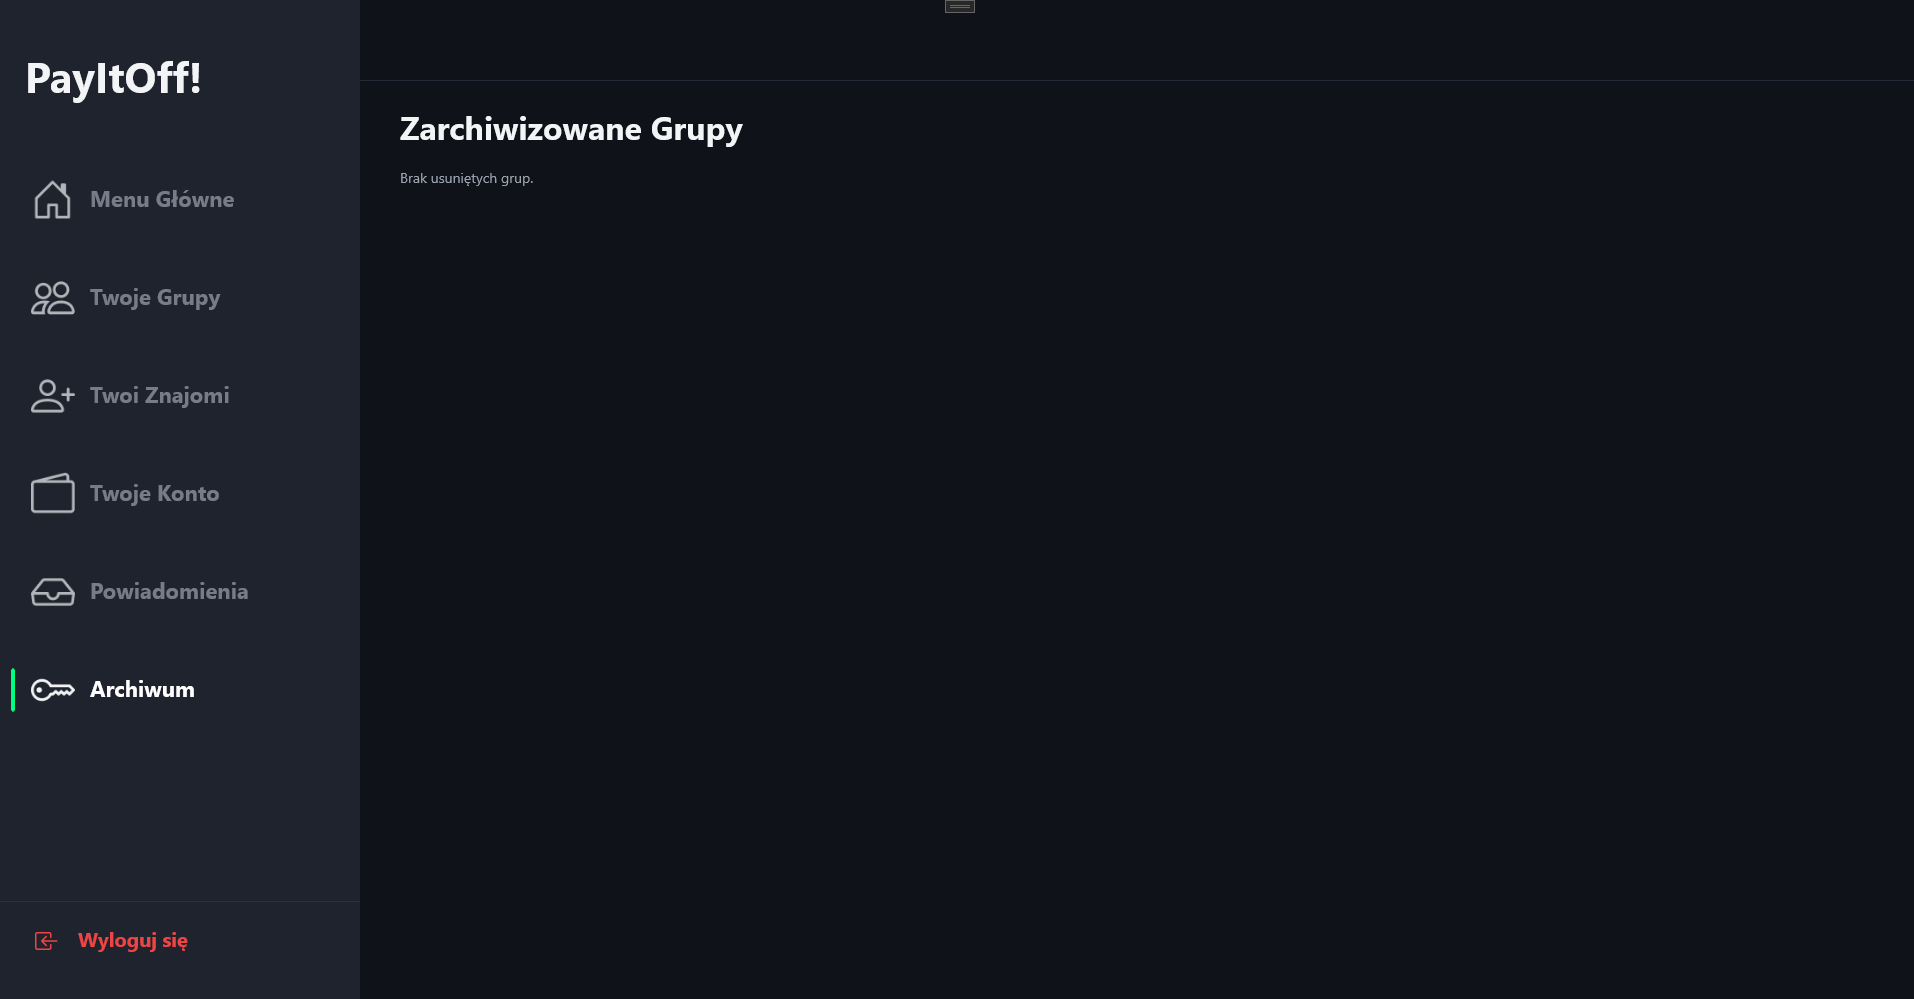
\includegraphics[width=0.95\textwidth]{img/archiwum/archiwum_pusty_widok.png}
    \vspace{0.5cm} \\
    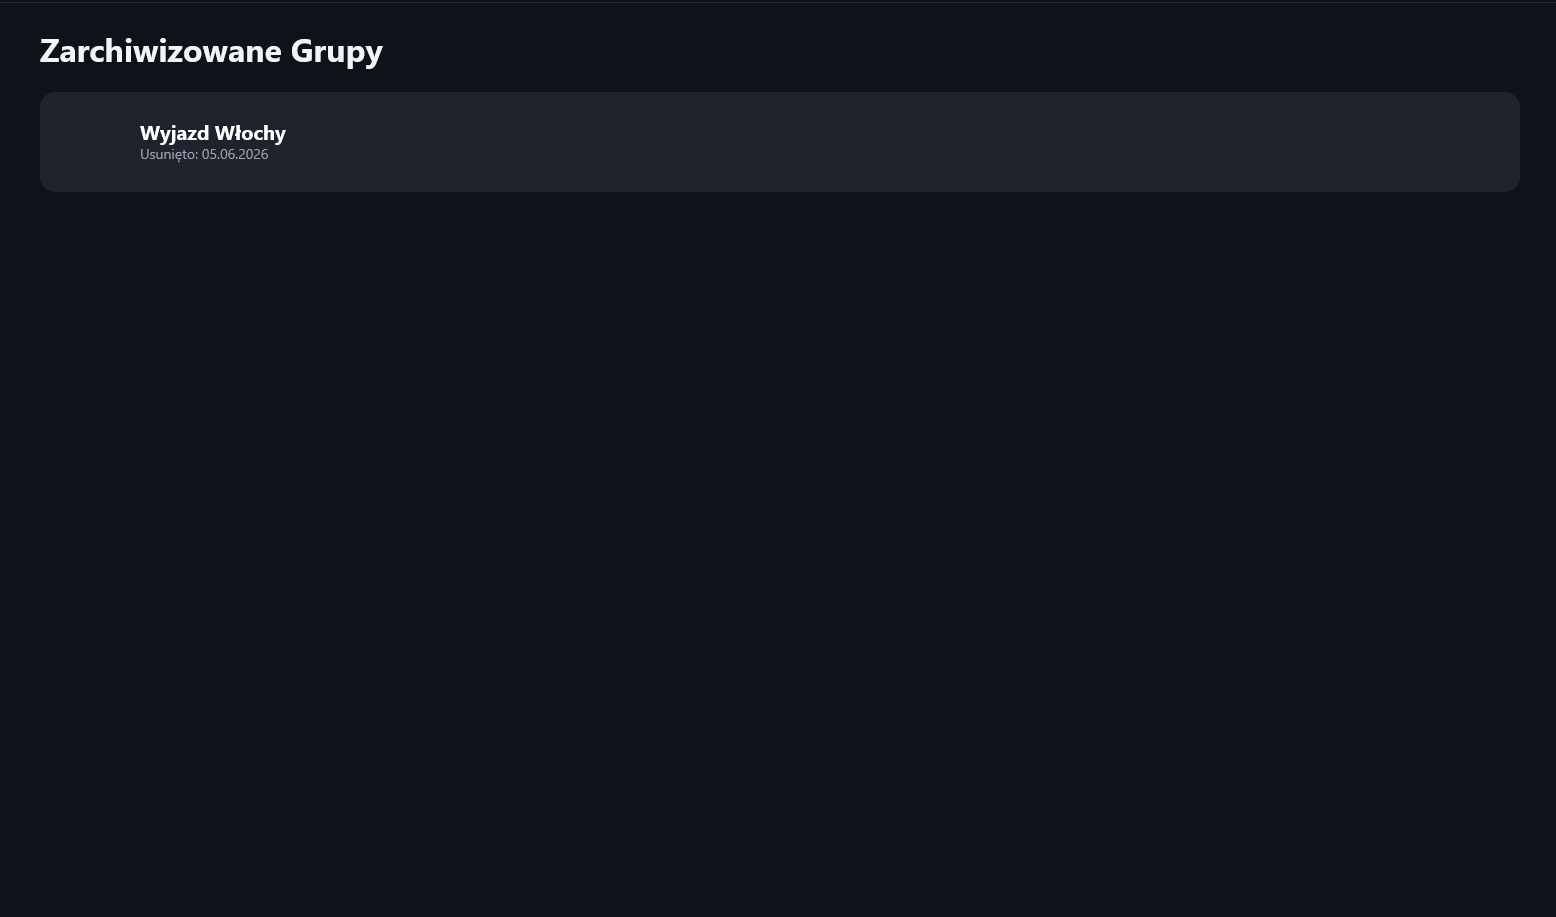
\includegraphics[width=0.95\textwidth]{img/archiwum/archiwum_usunieta_grupa.png}
    \vspace{0.5cm} \\
    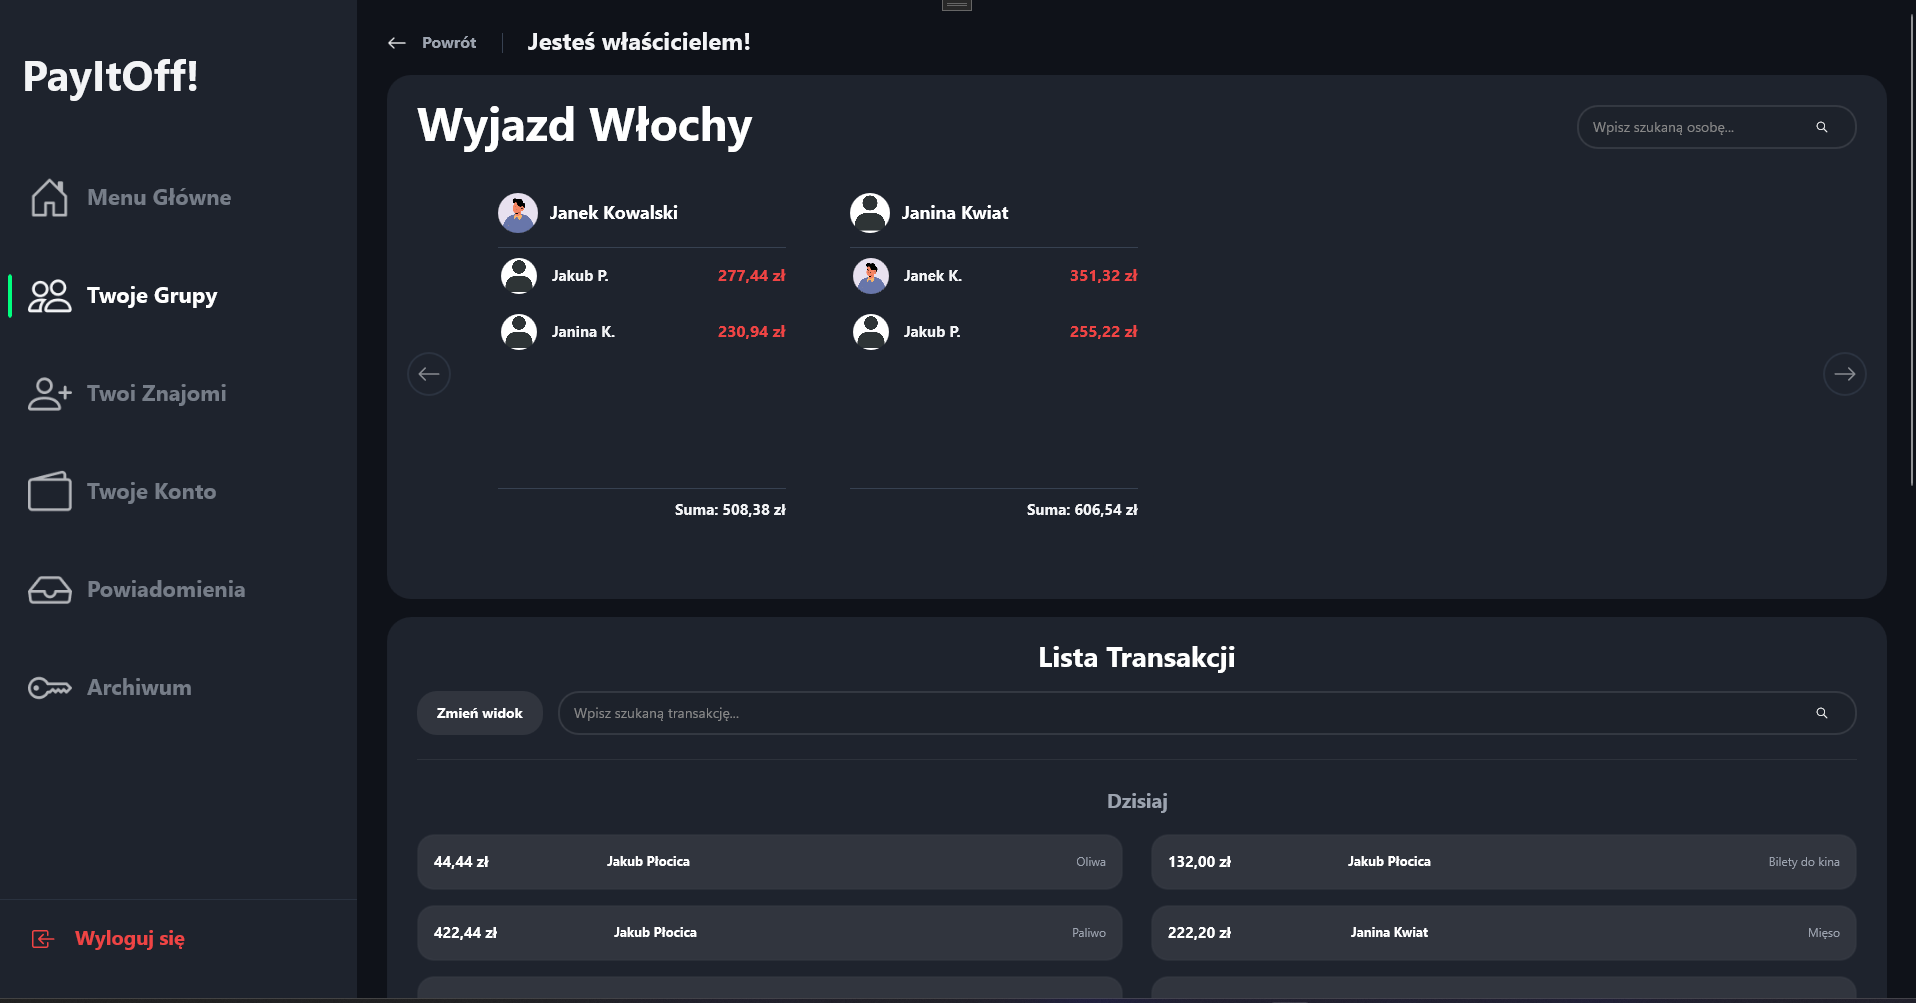
\includegraphics[width=0.95\textwidth]{img/archiwum/archiwum_grupa_read-only.png}
    \captionof{figure}{Zarządzanie retencją danych. Widok archiwum (pusty stan), wykaz usuniętych środowisk oraz odseparowany tryb "Tylko do odczytu" dla zarchiwizowanych grup wydatkowych.}
\end{center}

\section{Harmonogramowanie Zadań w Tle (Hangfire)}
Aby odciążyć główny wątek serwera API i zapewnić niezawodną realizację długotrwałych operacji, w projekcie wdrożono sprawdzoną bibliotekę \textbf{Hangfire}. 

Hangfire pozwala na bezpieczne kolejkowanie zadań asynchronicznych typu \textit{Fire-and-forget} oraz konfigurowanie zadań cyklicznych (\textit{Recurring jobs}). W systemie PayItOff biblioteka ta jest podłączona do docelowej bazy danych PostgreSQL, w której zapisuje swój wewnętrzny stan oraz listę operacji do wykonania. Dzięki wbudowanemu interfejsowi graficznemu \textit{Hangfire Dashboard} pod adresem \texttt{/hangfire}, deweloper może w czasie rzeczywistym podglądać aktywne procesy w tle, diagnozować błędy oraz ręcznie ponawiać przerwane zadania bez obaw o utratę danych.

\textbf{Praktyczne użycie w systemie - DailySummaryJob:}
Aplikacja PayItOff świadomie unika "spamowania" użytkownika powiadomieniami o każdym drobnym rachunku wprowadzanym przez znajomych w ciągu dnia. W tym celu mniejsze notyfikacje są początkowo oznaczane jako "ukryte". System Hangfire posiada zdefiniowane zadanie cykliczne skonfigurowane w klasie \texttt{Program.cs} za pomocą wyrażenia Cron: \texttt{"0 20 * * *"}. Oznacza to, że każdego dnia o godzinie 20:00 proces w tle wybudza klasę \texttt{DailySummaryJob}. Serwis ten pobiera wszystkie ukryte mikro-powiadomienia przypisane do danego użytkownika z ostatnich 24 godzin, usuwa je, agreguje ich treść i tworzy jedno potężne, zbiorcze powiadomienie typu \textit{DailySummary} ("Podsumowanie z dzisiaj"). Mechanizm ten działa w pełni asynchronicznie poza głównym wątkiem API, gwarantując wydajność aplikacji i czystość w skrzynce odbiorczej klienta.

\begin{center}
    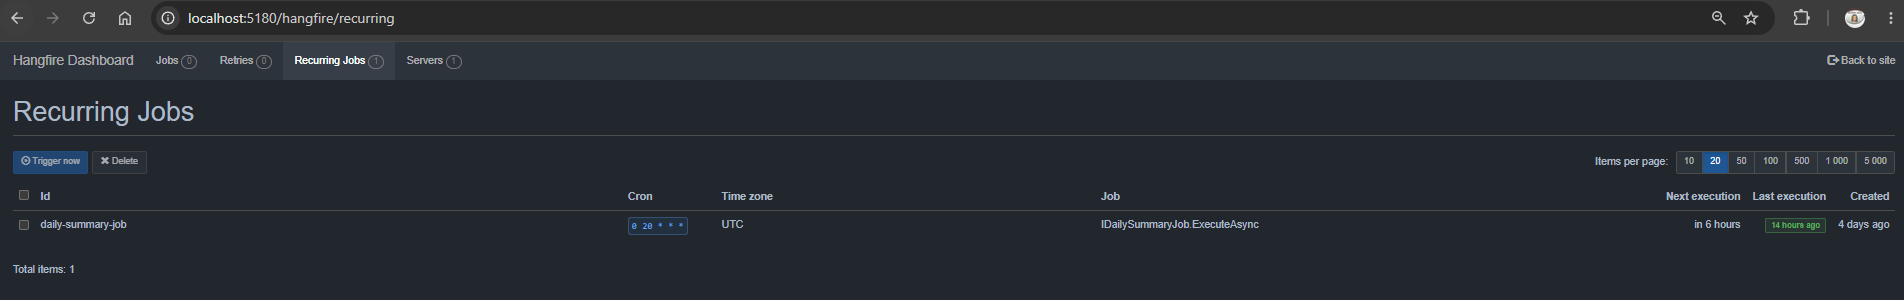
\includegraphics[width=0.95\textwidth]{img/hangfire.png}
    \captionof{figure}{Panel administracyjny biblioteki Hangfire. Interaktywny widok Dashboardu umożliwiający monitorowanie, wznawianie i zarządzanie kolejką zadań asynchronicznych w czasie rzeczywistym z poziomu przeglądarki.}
\end{center}

\section{Opis Wybranych Fragmentów Kodu Źródłowego}

\subsection{Algorytm dzielenia rachunku (Penny-Drop Problem)}
Poniższy kod znajduje się w klasie \texttt{DebtCalculator}. Odpowiada on za równe dzielenie kwoty między uczestników grupy. Głównym wyzwaniem było rozwiązanie tzw. problemu zgubionego grosza, czyli sytuacji, w której kwota nie dzieli się bez reszty (np. 10 zł na 3 osoby). Kod oblicza bazową część ułamkową i rozdziela resztę w postaci pojedynczych groszy, tak by każdy rachunek sumował się co do grosza.
\begin{center}
\begin{verbatim}
decimal baseAmount = Math.Floor((totalAmount / participantsCount) * 100) / 100;
decimal allocatedTotal = baseAmount * participantsCount;
decimal remainder = totalAmount - allocatedTotal;

int penniesToDistribute = (int)Math.Round(remainder * 100);
var sortedParticipants = participantIds.OrderBy(id => id).ToList();

for (int i = 0; i < participantsCount; i++)
{
    decimal amountForPerson = baseAmount;
    if (penniesToDistribute > 0)
    {
        amountForPerson += 0.01m;
        penniesToDistribute--;
    }
    // ... przypisanie ostatecznej wartości ułamkowej do osoby
}
\end{verbatim}
\captionof{figure}{Algorytm rozwiązywania problemu zgubionego grosza.}
\end{center}

\subsection{Logowanie i zapisywanie tokenu JWT}
W aplikacji klienckiej (.NET MAUI) za komunikację z serwerem i logowanie odpowiada serwis \texttt{AuthService}. Po udanym zapytaniu HTTP do API, serwer weryfikuje hasło i zwraca bezpieczny token JWT. Ten token jest przechowywany w bezpiecznym magazynie kluczy (SecureStorage), by uchronić go przed kradzieżą.
\begin{center}
\begin{verbatim}
public async Task<bool> LoginAsync(LoginRequest request)
{
    var response = await _httpClient.PostAsJsonAsync($"User/login", request);

    if (response.IsSuccessStatusCode)
    {
        var result = await response.Content.ReadFromJsonAsync<LoginResponse>();
        await SecureStorage.Default.SetAsync("jwt_token", result!.Token);
        return true;
    }
    else
    {
        var errorContent = await response.Content.ReadAsStringAsync();
        // wyłapanie błędu i poinformowanie użytkownika...
    }
}
\end{verbatim}
\captionof{figure}{Odbieranie i zabezpieczanie tokenu autoryzacyjnego.}
\end{center}

\subsection{Globalna Obsługa Błędów i Walidacja potoku HTTP}
Aby zachować maksymalną czystość kodu w kontrolerach i zapobiec wyciekowi niespodziewanych wyjątków na zewnątrz struktury API, zastosowano niestandardowe oprogramowanie pośredniczące (\textit{ExceptionMiddleware}). Przechwytuje ono każdy błąd na poziomie całego potoku, formatując go w ujednoliconą odpowiedź JSON. Kod połączono z architekturą \textbf{FluentValidation}, która automatycznie ocenia reguły biznesowe zanim żądanie w ogóle trafi do serwisów aplikacyjnych.
\begin{center}
\begin{verbatim}
public async Task InvokeAsync(HttpContext httpContext)
{
    try
    {
        await _next(httpContext);
    }
    catch (Exception ex)
    {
        await HandleExceptionAsync(httpContext, ex);
    }
}

// (...) Fragment metody HandleExceptionAsync:
if (ex is ValidationException validationEx)
{
    var errors = validationEx.Errors.Select(e => e.ErrorMessage);
    await response.WriteAsJsonAsync(new { 
        message = "Validation Failed", 
        errors = errors 
    });
}
\end{verbatim}
\captionof{figure}{Globalny system przechwytywania i ujednolicania błędów (ExceptionMiddleware).}
\end{center}

\subsection{Odpytywanie bazy przy użyciu Entity Framework}
Do obsługi zapytań bazodanowych w projekcie zastosowano wzorzec Repozytorium. Poniższy krótki fragment pochodzi z \texttt{GroupDebtRepository} i pokazuje użycie LINQ oraz zapytań asynchronicznych do bazy SQL. Sprawdza on z użyciem metody \texttt{AnyAsync}, czy w wybranej grupie istnieją jeszcze jakieś nieuregulowane długi.
\begin{center}
\begin{verbatim}
public async Task<bool> HasActiveGroupDebt(int groupId)
{
    return await _context.GroupDebts
        .Where(x => x.GroupId == groupId && x.Amount > 0)
        .AnyAsync();
}

public async Task<GroupDebt?> GetDebtAsync(int groupId, int debtorId, int creditorId)
{
    return await _context.GroupDebts
        .Where(x => x.GroupId == groupId && 
                    x.DebtorId == debtorId && 
                    x.CreditorId == creditorId)
        .FirstOrDefaultAsync();
}
\end{verbatim}
\captionof{figure}{Użycie Entity Framework Core do filtracji danych.}
\end{center}

\subsection{Tworzenie wydatków z użyciem Transakcji Bazy Danych}
Dodawanie pojedynczego paragonu wiąże się ze stworzeniem wielu powiązanych wpisów (wydatki, pozycje na paragonie, zaktualizowanie długów osób). Zastosowano więc bezpieczne transakcje bazodanowe. Uruchamiając metodę \texttt{BeginTransactionAsync}, mamy pewność, że jeśli w trakcie obliczania nastąpi błąd, system automatycznie anuluje zmiany (Rollback), aby baza nie pozostała w stanie uszkodzonym.
\begin{center}
\begin{verbatim}
public async Task CreateExpenseBatch(int userId, CreateExpenseBatchRequest request)
{
    var group = await _groupRepository.GetGroupInfoByIdAsync(request.GroupId);
    var creator = await _userRepository.GetUserByIdAsync(userId);

    await _unitOfWork.BeginTransactionAsync();
    try
    {
        // ... tworzenie i zapisywanie wydatku Expense
        
        await _unitOfWork.CommitAsync(); // Wszystko ok, zapisz zmiany
    }
    catch (Exception ex)
    {
        await _unitOfWork.RollbackAsync(); // Cofnij zmiany, zgłoś błąd
        throw;
    }
}
\end{verbatim}
\captionof{figure}{Obsługa wzorca Unit Of Work w operacjach kosztowych.}
\end{center}

\subsection{Architektura MVVM i powiązanie z interfejsem}
Aby kod w aplikacji mobilnej był czysty i łatwy w testowaniu, cały ekran ma oddelegowaną klasę \texttt{ViewModel}. Poniższy przykład pochodzi z \texttt{AddExpenseViewModel}. Dzięki bibliotece rozszerzeń \texttt{CommunityToolkit.Mvvm} i atrybutowi \texttt{[ObservableProperty]}, system sam wie, kiedy zmieniła się nazwa grupy czy wydatek i na tej podstawie od razu odświeża napisy w plikach widoku .xaml.
\begin{center}
\begin{verbatim}
public partial class AddExpenseViewModel : PopupViewModelBase, IQueryAttributable
{
    private readonly GroupService _groupService;

    [ObservableProperty]
    public partial int GroupId { get; set; }

    [ObservableProperty]
    public partial string GroupName { get; set; } = string.Empty;

    public ObservableCollection<ReceiptItem> BufferItems { get; } = new();

    public AddExpenseViewModel(GroupService groupService)
    {
        _groupService = groupService;
    }
}
\end{verbatim}
\captionof{figure}{Kod struktury ekranu przy użyciu wzorca MVVM.}
\end{center}

\subsection{Ewaluator Wyrażeń Matematycznych (Math Parser) w polu ceny}
Aby ułatwić użytkownikom wprowadzanie skomplikowanych rachunków prosto z paragonu (np. sumowanie cen wielu małych produktów), aplikacja udostępnia funkcję automatycznego przeliczania wyrażeń matematycznych (np. \texttt{5.50 + 2 * 3}) bezpośrednio w polu tekstowym. Użyto do tego wbudowanego silnika ewaluacji danych z biblioteki \texttt{System.Data}.
\begin{center}
\begin{verbatim}
private void ParseUnitPrice()
{
    try
    {
        if (string.IsNullOrWhiteSpace(_unitPriceInput)) { UnitPrice = 0; return; }
        
        string expression = _unitPriceInput.Replace(',', '.');
        var result = new System.Data.DataTable().Compute(expression, null);
        
        if (result != DBNull.Value && result != null)
        {
            UnitPrice = Math.Round(Convert.ToDecimal(result), 2);
        }
    }
    catch { /* Zignoruj błędne formaty podczas wpisywania */ }
}
\end{verbatim}
\captionof{figure}{Konwersja wyrażenia matematycznego z pola tekstowego w locie (Real-time Math Parser).}
\end{center}

\subsection{Reaktywny algorytm podziału kosztów na żywo (Client-Side)}
Zanim rachunek trafi do ostatecznej weryfikacji na serwerze API, klient MAUI udostępnia natychmiastowy, reaktywny podgląd "kto zapłaci ile" już w momencie zaznaczania osób. Kod z modelu \texttt{ReceiptModels.cs} dokonuje "Sprawiedliwego podziału co do grosza" (rozwiązując problem ułamków) w czasie rzeczywistym i aktualizuje widok.
\begin{center}
\begin{verbatim}
public void RecalculateShares()
{
    if (AssignedMembers.Count == 0) return;

    decimal share = Math.Round(TotalPrice / AssignedMembers.Count, 2);
    decimal totalAllocated = 0;

    foreach (var m in AssignedMembers)
    {
        m.OwedAmount = share;
        totalAllocated += share;
    }

    decimal remainder = TotalPrice - totalAllocated;
    if (remainder != 0 && AssignedMembers.Count > 0)
    {
        // Przypisz brakującego/nadmiarowego grosza pierwszej osobie
        var firstMember = AssignedMembers.First();
        firstMember.OwedAmount += remainder;
    }
}
\end{verbatim}
\captionof{figure}{Client-Side Penny Drop – podział rachunku i rozwiązanie reszty na żywo na froncie.}
\end{center}

\subsection{Automatyczna Iniekcja Tokenu JWT w aplikacji mobilnej}
Aplikacja .NET MAUI posiada zaawansowany mechanizm autoryzacji bazujący na klasie \texttt{DelegatingHandler}. Po zalogowaniu, aplikacja przechowuje token sesji w bezpiecznym magazynie \texttt{SecureStorage}. Poniższy kod przechwytuje każde żądanie HTTP wychodzące z klienta i automatycznie dokleja w nagłówku pobrany certyfikat Bearer, zapewniając bezobsługową autoryzację dla wszystkich widoków.
\begin{center}
\begin{verbatim}
public class AuthHandler : DelegatingHandler
{
    protected override async Task<HttpResponseMessage> SendAsync(
        HttpRequestMessage request, CancellationToken cancellationToken)
    {
        var token = await SecureStorage.Default.GetAsync("jwt_token");

        if (!string.IsNullOrEmpty(token))
        {
            request.Headers.Authorization = 
                new AuthenticationHeaderValue("Bearer", token);
        }

        return await base.SendAsync(request, cancellationToken);
    }
}
\end{verbatim}
\captionof{figure}{Wzorzec DelegatingHandler automatyzujący dołączanie nagłówka Authorization.}
\end{center}

\subsection{Powiadomienia E-mail przy użyciu MailKit i protokołu SMTP}
System powiadomień oparty jest nie tylko na alertach w aplikacji, ale również na prawdziwych wiadomościach e-mail przesyłanych do skrzynek pocztowych użytkowników. W tym celu w warstwie Aplikacji zastosowano zaawansowaną bibliotekę \texttt{MailKit}. Poniższy fragment serwisu zarządza nawiązaniem szyfrowanego połączenia TLS z zewnętrznym serwerem SMTP i uwierzytelnieniem nadawcy przed asynchroniczną wysyłką powiadomienia (np. o zaproszeniu do grupy).
\begin{center}
\begin{verbatim}
public async Task SendEmailAsync(string to, string subject, string body)
{
    var email = new MimeMessage();
    email.From.Add(new MailboxAddress("PayItOff", "no-reply@payitoff.com"));
    email.To.Add(MailboxAddress.Parse(to));
    email.Subject = subject;
    email.Body = new TextPart(TextFormat.Html) { Text = body };

    using var smtp = new SmtpClient();
    await smtp.ConnectAsync("smtp.server.com", 587, SecureSocketOptions.StartTls);
    await smtp.AuthenticateAsync("user", "password");
    await smtp.SendAsync(email);
    await smtp.DisconnectAsync(true);
}
\end{verbatim}
\captionof{figure}{Implementacja wysyłki maili z poziomu serwera C\# używając standardu MimeMessage.}
\end{center}

\subsection{Dostosowanie platformy Windows (MAUI Desktop Handlers)}
Aplikacja .NET MAUI działa wieloplatformowo, jednak by zachować nowoczesny wygląd na komputerach osobistych (Desktop), w klasie \texttt{MauiProgram.cs} zaimplementowano niestandardowe handlery (Mappery) pod platformę Windows. Dzięki kompilacji warunkowej \texttt{\#if WINDOWS}, system nadpisuje domyślne zachowania formantów takich jak \texttt{Entry}, \texttt{Picker} czy \texttt{Editor}, usuwając natywne obramowania systemu Windows i zapobiegając niepożądanemu przewijaniu interfejsu w górę po kliknięciu (\texttt{PreventScrollOnFocus}).
\begin{center}
\begin{verbatim}
Microsoft.Maui.Handlers.EntryHandler.Mapper.AppendToMapping("NoBorder", (h, v) =>
{
#if WINDOWS
    h.PlatformView.BorderThickness = new Microsoft.UI.Xaml.Thickness(0);
    h.PlatformView.Background = new Microsoft.UI.Xaml.Media.SolidColorBrush(
        Microsoft.UI.Colors.Transparent);
    h.PlatformView.BorderBrush = new Microsoft.UI.Xaml.Media.SolidColorBrush(
        Microsoft.UI.Colors.Transparent);
        
    h.PlatformView.GotFocus += (s, e) =>
    {
        h.PlatformView.BorderThickness = new Microsoft.UI.Xaml.Thickness(0);
    };
#endif
});
\end{verbatim}
\captionof{figure}{Modyfikacja natywnych formantów systemu Windows w locie.}
\end{center}

\section{Instrukcja Uruchomienia Aplikacji}
Aby poprawnie uruchomić system PayItOff, należy skonfigurować i uruchomić obie jego warstwy: serwerową (API wraz z bazą danych) oraz kliencką (.NET MAUI).

\subsection{Wymagania wstępne}
\begin{itemize}
    \item Zainstalowane środowisko uruchomieniowe \textbf{.NET 10 SDK}.
    \item Zainstalowane IDE \textbf{Visual Studio 2026} z włączonymi obciążeniami roboczymi (workloads): \textit{ASP.NET and web development} oraz \textit{.NET Multi-platform App UI development}.
    \item Zainstalowane i uruchomione narzędzie \textbf{Docker Desktop} (niezbędne do konteneryzacji bazy danych i serwera API).
\end{itemize}

\subsection{Krok 1: Uruchomienie Serwera i Bazy Danych (Backend)}
Zarządzanie środowiskiem serwerowym oraz bazą danych odbywa się za pomocą środowisk kontenerowych, co wyklucza typowe problemy z konfiguracją środowiska lokalnego u różnych programistów.
\begin{enumerate}
    \item Otwórz terminal (wiersz poleceń) w głównym katalogu pobranej solucji (w miejscu, gdzie znajduje się plik \texttt{docker-compose.yml}).
    \item Wywołaj polecenie budujące i uruchamiające całą infrastrukturę w tle:
    \begin{verbatim}
    docker-compose up -d --build
    \end{verbatim}
    \item Proces ten pobierze odpowiednie obrazy systemowe, uruchomi relacyjną bazę danych, a następnie zaimplementuje migracje struktury bazy (Entity Framework). Serwer Web API rozpocznie nasłuchiwanie żądań HTTP.
\end{enumerate}
\textit{Alternatywa deweloperska:} Serwer API można również uruchomić bezpośrednio z poziomu Visual Studio, wybierając projekt \texttt{PayItOff.Api} jako startowy (np. profil \texttt{http} / \texttt{https}), przy czym kontener z samą bazą danych nadal musi być aktywny.

\subsection{Krok 2: Uruchomienie Klienta Desktopowego (.NET MAUI)}
Gdy serwer API działa i nasłuchuje na wskazanym porcie, należy uruchomić interfejs graficzny aplikacji:
\begin{enumerate}
    \item Otwórz główny plik solucji (\texttt{PayItOff.sln}) w środowisku Visual Studio 2026.
    \item W oknie \textit{Solution Explorer} zlokalizuj projekt kliencki o nazwie \textbf{\texttt{PayItOff.MauiClient}}.
    \item Kliknij na niego prawym przyciskiem myszy i wybierz opcję \textbf{Set as Startup Project} (Ustaw jako projekt startowy).
    \item Na górnym pasku narzędzi uruchamiania (w sekcji \textit{Framework Target}) upewnij się, że wybrano maszynę docelową: \textbf{Windows Machine}.
    \item Rozpocznij proces kompilacji i debugowania wciskając klawisz \texttt{F5} (lub zielony przycisk Play).
    \item Aplikacja skompiluje widoki XAML, uruchomi się jako natywny program okienkowy Windows i nawiąże połączenie z uruchomionym wcześniej lokalnym serwerem backendowym.
\end{enumerate}

\section{Repozytorium GitHub}
Cały kod źródłowy aplikacji (zarówno serwer API, warstwa bazy danych, jak i sama aplikacja MAUI) znajduje się w moim prywatnym / uczelnianym repozytorium:
\begin{itemize}
    \item \textbf{Link do projektu:} \url{https://github.com/Kaparee/PayItOff}
\end{itemize}

\section{Podsumowanie i Wnioski}
Projekt PayItOff to system do kompleksowego monitorowania i zarządzania finansami grupowymi, usprawniający proces rozliczania kosztów i długów między znajomymi.

\textbf{Główne osiągnięcia projektu:}
\begin{itemize}
    \item \textbf{Interfejs użytkownika:} Stworzono intuicyjne panele mobilne i desktopowe oparte o .NET MAUI i wzorzec MVVM, zapewniające efektywne zarządzanie wydatkami.
    \item \textbf{Zarządzanie wydatkami:} System umożliwia tworzenie grup, dodawanie rachunków, przeliczanie długów w czasie rzeczywistym oraz odnotowywanie spłat.
    \item \textbf{Bezpieczeństwo danych:} Wdrożono bezpieczne logowanie oparte na tokenach JWT oraz hashowanie haseł w celu ochrony danych użytkowników.
    \item \textbf{Trwałość danych:} Zapewniono stabilne przechowywanie danych w relacyjnej bazie dzięki frameworkowi Entity Framework Core i wbudowanej transakcyjności.
    \item \textbf{Modułowa architektura:} Zastosowano warstwową architekturę (Clean Architecture) z wzorcem repozytorium i wstrzykiwaniem zależności (Dependency Injection), co poprawiło czytelność i rozszerzalność kodu.
    \item \textbf{Walidacja i algorytmika:} Zaimplementowano zaawansowaną walidację danych oraz matematyczną logikę podziału kwot (unikanie błędu ułamków), aby zapewnić absolutną integralność finansową.
\end{itemize}

\textbf{Wyzwania i wnioski:} \\
Realizacja projektu pozwoliła na zdobycie praktycznego doświadczenia w zakresie tworzenia projektów typu klient-serwer, wstrzykiwania zależności, zarządzania asynchronicznością i transakcjami bazodanowymi oraz projektowania interfejsów użytkownika. Tworzenie projektu znacząco poszerzyło umiejętności w budowaniu stabilnych i bezpiecznych aplikacji rozproszonych.

\textbf{Potencjalny rozwój:} \\
System może być w przyszłości rozbudowany o kilka rzeczy, głównie o integrację z prawdziwymi bramkami płatności (np. BLIK), półautomatyczne skanowanie paragonów przy użyciu modułu OCR oraz bardziej zaawansowane statystyki wydatków.

\end{document}





